% =============================================================
% บทที่ 4 การวิเคราะห์ระบบ และพัฒนาโปรแกรม
% =============================================================

% -----------------------------------------------------------
\section{การวิเคราะห์ระบบ}
% -----------------------------------------------------------

บทนี้ศึกษาทำความเข้าใจปัญหาและความต้องการของผู้มีส่วนได้ส่วนเสีย การกำหนดขอบเขตและคุณลักษณะที่ระบบต้องตอบสนอง และสังเคราะห์ประเด็นข่าวภาษาไทย

\subsection{ผู้ใช้งานระบบและสิทธิ์การเข้าถึง}

ผู้ใช้งานระบบได้รับการจำแนกออกเป็น 3 กลุ่มหลัก ดังแสดงในตารางที่~\ref{tab_roles_permissions}

\begin{table}[H]
\centering
\caption{บทบาทและสิทธิ์การเข้าถึงระบบ}
\label{tab_roles_permissions}
\resizebox{\textwidth}{!}{%
\begin{tabular}{|L{3.5cm}|L{11.0cm}|}
\hline
\textbf{บทบาท} & \textbf{สิทธิ์การเข้าถึงและการใช้งานระบบ} \\
\hline
ผู้อ่านข่าวทั่วไป\newline (Reader) & เข้าถึงหน้าหลัก Bento Hub ผ่านเว็บเบราว์เซอร์ เรียกดูรายการข่าวสารสดประจำวัน กรองข่าวสารตาม 9 หมวดหมู่หลักและสำนักพิมพ์ ค้นหาข่าวสารด้วยคำสำคัญ เปิดพรีวิวเนื้อหาข่าวในตัวเว็บ (In-App Reader) พร้อมลิงก์ไปยังต้นฉบับเพื่อเคารพลิขสิทธิ์ อ่านบทสรุปเนื้อหาและผลวิเคราะห์อารมณ์ที่สังเคราะห์จากบทความฉบับเต็มด้วยโมเดลภาษาขนาดใหญ่ สำรวจประเด็นข่าวยอดนิยม 6 มิติ สำรวจแฟ้มมหากาพย์ประเด็นข่าวและไทม์ไลน์พัฒนาการเหตุการณ์ บันทึกคั่นหน้าบทความที่สนใจ เรียกดูประวัติการอ่าน และจัดการสิทธิ์ความเป็นส่วนตัวและคุกกี้ตามมาตรฐาน PDPA \\ \hline
ผู้ดูแลระบบ\newline (Administrator) & เข้าสู่ศูนย์ควบคุมและติดตามสถานะระบบ (Ops Monitoring Console) ด้วยรหัสผ่านลับ ตรวจสอบสถานะการทำงาน สถิติ Throughput การใช้หน่วยความจำ และสถานะการทำงานของแคช สั่งเริ่มรอบการดึงข่าวด่วนทันที (Scrape Now) สั่งล้างแคชในหน่วยความจำและแคช HTTP (Clear Cache) ทดสอบการเชื่อมต่อและดึงข้อมูลของสำนักข่าวรายแห่ง (Test Source Probe) และตรวจสอบความสอดคล้องของคลังข้อมูล Single Source of Truth \\ \hline
ระบบตั้งเวลาและประมวลผลเบื้องหลัง\newline (Automated Scheduler) & ทำงานอัตโนมัติตามรอบเวลา ดึงข้อมูลข่าวสารจากสำนักข่าวออนไลน์ทุกแห่งที่ลงทะเบียนผ่าน Playwright และ HTTP ดำเนินการตัดคำภาษาไทย ทำความสะอาดข้อความ และจำแนก 9 หมวดหมู่ สกัดเวกเตอร์ความหมาย 768 มิติและเอนทิตีชื่อเฉพาะ ระบุและรวมกลุ่มจุลเหตุการณ์ออนไลน์ (Stage A) เชื่อมโยงเข้าสู่เส้นเรื่องมหาภาค (Stage B) คำนวณคะแนนกระแสข่าว 6 มิติเชิงสถิติ บังคับใช้เกตป้องกันข้อมูลเท็จ 3 ชั้น บันทึกข้อมูลลงฐานข้อมูล SQLite WAL และไฟล์ JSON พร้อมทั้งกระจายสัญญาณข่าวสดไปยังเบราว์เซอร์ผ่าน WebSocket \\
\hline
\end{tabular}%
}
\end{table}

\subsection{ความต้องการเชิงฟังก์ชัน}

ความต้องการเชิงฟังก์ชัน (Functional Requirements) กำหนดความสามารถและหน้าที่ที่ระบบต้องปฏิบัติตามความต้องการของผู้ใช้งานและระบบเบื้องหลัง ครอบคลุม 15 ข้อกำหนดหลัก (FR-01 ถึง FR-15) ดังแสดงในตารางที่~\ref{tab_functional_requirements}

\begin{longtable}{|C{1.3cm}|L{3.6cm}|L{6.0cm}|L{1.8cm}|}
\caption{ความต้องการเชิงฟังก์ชันของระบบ}\label{tab_functional_requirements}\\
\hline
\textbf{รหัส} & \textbf{ความต้องการเชิงฟังก์ชัน} & \textbf{รายละเอียดความสามารถของระบบ} & \textbf{ผู้ใช้} \\ \hline
\endfirsthead
\caption[]{ความต้องการเชิงฟังก์ชันของระบบ~\cskkuContinued}\\
\hline
\textbf{รหัส} & \textbf{ความต้องการเชิงฟังก์ชัน} & \textbf{รายละเอียดความสามารถของระบบ} & \textbf{ผู้ใช้} \\ \hline
\endhead
FR-01 & การดึงข่าวอัตโนมัติหลายสำนัก & ระบบสามารถดึงข้อมูลข่าวสารจากสำนักข่าวออนไลน์หลากหลายแห่ง ทั้งแบบ RSS Feed, เว็บไซต์ HTML ปกติ และเว็บไซต์ที่เรนเดอร์ด้วย JavaScript ผ่าน Playwright โดยไม่บล็อกการทำงานหลัก & ระบบอัตโนมัติ \\ \hline
FR-02 & การลงทะเบียนแหล่งข่าวแบบไดนามิก & ระบบรองรับการเพิ่มและปรับปรุงแหล่งข่าวใหม่ผ่าน Decorator (@register\_source) พร้อมกำหนดคู่สีของสำนักข่าวและตรวจสอบความถูกต้องก่อนเริ่มงาน & ผู้ดูแลระบบ \\ \hline
FR-03 & การจำแนกหมวดหมู่ภาษาไทย 9 หมวด & ระบบสามารถตัดคำ ทำความสะอาดข้อความ และจำแนกข่าวภาษาไทยออกเป็น 9 หมวดหมู่อย่างถูกต้องด้วยเทคนิค 3-Tier Cascade Classifier & ระบบอัตโนมัติ \\ \hline
FR-04 & การสรุปข่าวและวิเคราะห์อารมณ์ & ระบบสามารถสร้างบทสรุปย่อ ประเด็นสำคัญ และวิเคราะห์อารมณ์ของข่าว (Sentiment) ด้วยโมเดลภาษาขนาดใหญ่ผ่าน KKU Gen.AI API พร้อมกลไกสำรอง & ผู้อ่านทั่วไป \\ \hline
FR-05 & การแสดงผลข่าวสดบน Bento Hub & ระบบนำเสนอข่าวสารผ่านหน้าเว็บ Bento Hub แบบ 3 มุมมอง มีแบนเนอร์แจ้งเตือนข่าวใหม่ลอยตัว และกระจายสัญญาณสดผ่าน Socket.IO โดยไม่ต้องรีเฟรชหน้าจอ & ผู้อ่านทั่วไป \\ \hline
FR-06 & การกรองข่าวและการสืบค้นคำสำคัญ & ระบบรองรับการกรองข่าวตาม 9 หมวดหมู่ กรองตามสำนักข่าว ค้นหาด้วยคำสำคัญแบบ Real-time และการสืบค้นขั้นสูงบนระบบเจาะประเด็นข่าว & ผู้อ่านทั่วไป \\ \hline
FR-07 & การอ่านพรีวิวเนื้อหาในตัวเว็บ & ระบบมีหน้าต่างแสดงผลพรีวิวเนื้อหาข่าวบางส่วน (In-App Modal Reader) ที่ผ่านการทำความสะอาดด้วย Trafilatura พร้อมลิงก์ไปยังต้นฉบับเพื่อความปลอดภัยด้านลิขสิทธิ์ และปุ่มสังเคราะห์สรุปเนื้อหาฉบับเต็มด้วย AI & ผู้อ่านทั่วไป \\ \hline
FR-08 & การบันทึกคั่นหน้าและประวัติการอ่าน & ระบบเปิดให้ผู้ใช้บันทึกคั่นหน้าข่าวที่สนใจและเรียกดูประวัติการอ่านย้อนหลัง โดยจัดเก็บข้อมูลบน LocalStorage ของเบราว์เซอร์ ปราศจากการระบุตัวตน & ผู้อ่านทั่วไป \\ \hline
FR-09 & การระบุประเด็นข่าวออนไลน์แบบคงทน & ระบบสามารถรวมข่าวที่รายงานเหตุการณ์เดียวกันเข้าสู่กลุ่มประเด็นข่าวออนไลน์ผ่านเกณฑ์ Two-Band Cosine Gate และปรับปรุง Centroid ด้วย EMA ข้ามหน้าต่าง 72 ชม. & ระบบอัตโนมัติ \\ \hline
FR-10 & การจัดอันดับกระแสข่าวสาร 6 มิติ & ระบบจัดอันดับประเด็นข่าวด้วย 6 มิติเชิงคณิตศาสตร์ ไม่ใช้ LLM ในการคำนวณคะแนน พร้อมกลไกลดทอนข่าวประจำวัน (Routine Penalty) และแจกแจงคะแนน & ผู้อ่านทั่วไป \newline ระบบอัตโนมัติ \\ \hline
FR-11 & การเชื่อมโยงเส้นเรื่องมหาภาค & ระบบเชื่อมโยงประเด็นข่าวย่อยข้ามสัปดาห์เข้าสู่มหากาพย์เหตุการณ์ผ่านคะแนนร่วม 4 ปัจจัย บังคับใช้กฎ Province-Only Veto และยกเว้นลดทอนเวลาในภาวะวิกฤต & ระบบอัตโนมัติ \\ \hline
FR-12 & แฟ้มสังเคราะห์ไทม์ไลน์และข้อเท็จจริง & ระบบสังเคราะห์ภาพรวม ไทม์ไลน์พัฒนาการ และตารางข้อเท็จจริงยืนยันข้ามสำนักข่าว (Corroborated Facts) พร้อมระบบตรวจทานรหัสอ้างอิงรายประโยค & ผู้อ่านทั่วไป \\ \hline
FR-13 & กลไกควบคุมความถูกต้อง 3 ระดับ & ระบบคัดกรองความเกี่ยวข้อง สกัด Typed Evidence และจัดสรรโหมดสังเคราะห์ 3 โหมด (halted\_mismatch, single\_source, synthesized) ป้องกันข้อมูลเท็จ & ระบบอัตโนมัติ \\ \hline
FR-14 & ศูนย์ควบคุมสถานะและการล้างแคช & ระบบมีหน้าต่างคอนโซลสำหรับผู้ดูแลระบบ ตรวจสอบ Throughput สั่งเริ่มสเกรปข่าวด่วนทันที ล้างแคช L1 และแคช HTTP และทดสอบสำนักข่าวรายแห่ง & ผู้ดูแลระบบ \\ \hline
FR-15 & การคุ้มครองข้อมูลส่วนบุคคล PDPA & ระบบประมวลผลคะแนนการมีส่วนร่วมแบบนิรนาม ไม่เก็บข้อมูลส่วนบุคคล มีแถบขอความยินยอมคุกกี้ และมีปุ่มล้างสถิติความสนใจออกจากเบราว์เซอร์ได้ทันที & ผู้อ่านทั่วไป \\
\hline
\end{longtable}

\subsection{ความต้องการที่ไม่ใช่เชิงฟังก์ชัน}

ความต้องการที่ไม่ใช่เชิงฟังก์ชัน (Non-Functional Requirements) กำหนดคุณสมบัติเชิงคุณภาพ ขีดความสามารถ และข้อจำกัดทางวิศวกรรมของระบบ ครอบคลุม 8 มิติสำคัญ (NFR-01 ถึง NFR-08) ดังแสดงในตารางที่~\ref{tab_non_functional_requirements}

\begin{table}[H]
\centering
\caption{ความต้องการที่ไม่ใช่เชิงฟังก์ชันของระบบ}
\label{tab_non_functional_requirements}
\resizebox{\textwidth}{!}{%
\begin{tabular}{|c|L{4.5cm}|L{9.5cm}|}
\hline
\textbf{รหัส} & \textbf{ด้าน} & \textbf{เกณฑ์คุณลักษณะที่กำหนด} \\
\hline
NFR-01 & ด้านเวลาตอบสนองของระบบ\newline (Performance Latency) & เวลาในการตอบสนองคำขอเรียกดูรายการข่าวผ่าน REST API (\texttt{GET /api/news}) ต้องมีค่าเฉลี่ยต่ำกว่า 150 มิลลิวินาทีเมื่อมีข้อมูลจัดเก็บในหน่วยความจำแคช \\ \hline
NFR-02 & ด้านความหน่วงเวลาผลักดันข้อมูลสด\newline (WebSocket Latency) & ความหน่วงเวลาในการกระจายข่าวสารใหม่และการแจ้งเตือนผ่าน Socket.IO ต้องต่ำกว่า 500 มิลลิวินาทีนับจากช่วงเวลาที่ข่าวได้รับการบันทึกลงระบบสำเร็จ \\ \hline
NFR-03 & ด้านอัตราการดึงข้อมูลและ Throughput\newline (Scraping Throughput) & ระบบต้องสามารถรองรับการดึงและสกัดเนื้อหาข่าวสารจากหลายสำนักพร้อมกันได้ในอัตราไม่น้อยกว่า 100 บทความต่อนาทีในสภาวะโหลดสูงสุด \\ \hline
NFR-04 & ด้านความคงทนและการแยกความเสียหาย\newline (Fault Isolation) & ความล้มเหลวในการเชื่อมต่อหรือโครงสร้างหน้าเว็บเปลี่ยนไปของสำนักข่าวใดสำนักข่าวหนึ่ง ต้องไม่ส่งผลกระทบต่อรอบการทำงานของสำนักข่าวอื่น \\ \hline
NFR-05 & ด้านความพร้อมใช้งานของระบบ\newline (System Availability) & ระบบต้องสามารถเปิดให้บริการอย่างต่อเนื่องตลอด 24 ชั่วโมงต่อวัน โดยมีอัตราความพร้อมใช้งานของระบบโดยรวมไม่ต่ำกว่าร้อยละ 99.5 ต่อเดือน \\ \hline
NFR-06 & ด้านความแม่นยำในการระบุเหตุการณ์\newline (Identification Accuracy) & ระบบระบุประเด็นข่าวต้องมีค่าความแม่นยำ B-cubed Precision ไม่ต่ำกว่า 0.85 และค่า B-cubed F1-score ไม่ต่ำกว่า 0.75 บนชุดข้อมูลทดสอบมาตรฐาน \\ \hline
NFR-07 & ด้านความมั่นคงปลอดภัยและความเป็นส่วนตัว\newline (Security \& Data Privacy) & ระบบต้องยึดหลัก Zero-PII ปราศจากการเก็บข้อมูลระบุตัวตน มีระบบ Rate Limiting, CORS Whitelist และส่วนหัวความปลอดภัย HTTP ป้องกัน XSS และ Clickjacking \\ \hline
NFR-08 & ด้านการทำงานข้ามแพลตฟอร์ม\newline (Cross-Platform Compatibility) & ซอฟต์แวร์ต้องสามารถรันได้อย่างสมบูรณ์ทั้งบนสภาพแวดล้อม Windows ในขั้นตอนการพัฒนา และสภาพแวดล้อม Linux Ubuntu บนคลาวด์สำหรับโพรดักชันจริง \\
\hline
\end{tabular}%
}
\end{table}

\subsection{กฎการตรวจสอบความถูกต้องของข้อมูล}

เพื่อรักษาความสมบูรณ์ ความถูกต้อง และความมั่นคงปลอดภัยของข้อมูลที่ไหลเวียนในระบบ ระบบได้กำหนดกฎเกณฑ์การตรวจสอบความถูกต้องของข้อมูล (Validation Rules) อย่างเข้มงวดผ่านโมเดล Pydantic v2 ครอบคลุม 10 กฎสำคัญ (VR-01 ถึง VR-10) ดังแสดงในตารางที่~\ref{tab_validation_rules}

\begin{table}[H]
\centering
\caption{กฎการตรวจสอบความถูกต้องของข้อมูล}
\label{tab_validation_rules}
\resizebox{\textwidth}{!}{%
\begin{tabular}{|c|L{4.2cm}|L{9.8cm}|}
\hline
\textbf{รหัส} & \textbf{ข้อมูลที่ตรวจสอบ} & \textbf{กฎการตรวจสอบความถูกต้องและข้อกำหนด} \\
\hline
VR-01 & URL บทความข่าว (\texttt{url}) & ต้องเป็นรูปแบบ URL ที่ถูกต้องตาม RFC 3986 ขึ้นต้นด้วย http หรือ https และมีความยาวไม่เกิน 2,048 อักขระ \\ \hline
VR-02 & หัวข้อบทความข่าว (\texttt{title}) & ต้องเป็นข้อความสตริงที่ไม่ว่างเปล่า มีความยาวระหว่าง 5 ถึง 500 อักขระ และผ่านการตัดอักขระความกว้างศูนย์ \\ \hline
VR-03 & สำนักข่าวต้นทาง (\texttt{source}) & ต้องตรงกับรายชื่อสำนักข่าวที่ลงทะเบียนไว้ใน Source Registry และเปิดใช้งานอยู่ในระบบเท่านั้น \\ \hline
VR-04 & หมวดหมู่ข่าว (\texttt{category}) & ต้องตรงกับ 1 ใน 9 หมวดหมู่หลักที่ระบบกำหนด ได้แก่ politics, economy, tech, crime, entertainment, sport, world, environment, social \\ \hline
VR-05 & วันเวลาเผยแพร่ (\texttt{published\_at}) & ต้องอยู่ในรูปแบบวันเวลามาตรฐาน ISO 8601 ที่ถูกต้อง และต้องไม่เป็นเวลาในอนาคตเกิน 1 ชั่วโมงเทียบกับเซิร์ฟเวอร์ \\ \hline
VR-06 & เวกเตอร์ความหมาย (\texttt{centroid}) & ต้องเป็นอาเรย์ของตัวเลขทศนิยมขนาด 768 มิติพอดี และต้องผ่านการปรับขนาดเวกเตอร์ให้เป็น 1 หน่วย (L2 Normalized) \\ \hline
VR-07 & ความคล้ายคลึงโคไซน์ (\texttt{cosine}) & ต้องเป็นตัวเลขทศนิยมที่มีค่าอยู่ในช่วงทางคณิตศาสตร์ตั้งแต่ -1.0 ถึง 1.0 เสมอ \\ \hline
VR-08 & รหัสผ่านลับผู้ดูแล (\texttt{secret}) & ต้องเป็นสตริงที่ไม่ว่างเปล่า มีความยาวไม่น้อยกว่า 8 อักขระ และตรวจสอบเทียบเคียงด้วยเวลาคงที่เพื่อป้องกัน Timing Attack \\ \hline
VR-09 & เหตุการณ์การมีส่วนร่วม (\texttt{action}) & ต้องระบุประเภทการกระทำที่ระบบยอมรับเท่านั้น ได้แก่ click, summary\_view, bookmark หรือ share \\ \hline
VR-10 & ส่วนหัวยืนยันตัวตน (\texttt{Authorization}) & ต้องระบุรูปแบบ Bearer Token ที่ถูกต้องตามมาตรฐาน RFC 6750 และเป็นโทเค็นเซสชันที่ยังไม่หมดอายุในหน่วยความจำ \\
\hline
\end{tabular}%
}
\end{table}

\subsection{แผนภาพกรณีใช้งาน}

การออกแบบพฤติกรรมของระบบจากมุมมองภายนอกนำเสนอผ่านแผนภาพกรณีใช้งาน (Use Case Diagram) ซึ่งจำแนกออกเป็น 2 มุมมองหลักตามบทบาทของผู้ใช้ ได้แก่ แผนภาพกรณีใช้งานสำหรับผู้อ่านข่าวทั่วไป (Reader) และแผนภาพกรณีใช้งานสำหรับระบบอัตโนมัติและผู้ดูแลระบบ (Scheduler \& Admin)

\subsubsection{แผนภาพกรณีใช้งานสำหรับผู้อ่านข่าวทั่วไป}

ผู้อ่านข่าวทั่วไปสามารถเข้าถึงบริการข้อมูลข่าวสาร สำรวจกระแส และใช้งานเครื่องมืออ่านข่าวผ่านเบราว์เซอร์ ดังแสดงในภาพที่~\ref{fig_usecase_reader}

\begin{figure}[H]
\centering
\begin{tikzpicture}[
    font=\small,
    actor/.style={draw, thick, circle, minimum size=0.45cm, inner sep=0pt},
    usecase/.style={draw, thick, ellipse, minimum width=4.8cm, minimum height=0.68cm, align=center, fill=white},
    sysbox/.style={draw, thick, dashed, rectangle, rounded corners=6pt, inner sep=12pt, fill=gray!3}
]

% Stickman Reader
\node[actor] (rhead) at (-5.0, 0) {};
\draw[thick] (rhead.south) -- ++(0, -0.6) coordinate (rtorso);
\draw[thick] ($(rhead.south)!0.3!(rtorso)$) -- ++(-0.35, -0.2);
\draw[thick] ($(rhead.south)!0.3!(rtorso)$) -- ++(0.35, -0.2);
\draw[thick] (rtorso) -- ++(-0.3, -0.55);
\draw[thick] (rtorso) -- ++(0.3, -0.55);
\node[below=0.6cm of rtorso, align=center] {\textbf{ผู้อ่านข่าวทั่วไป}\\\textbf{(Reader)}};

% Use Cases Reader
\node[usecase] (uc1) at (1.5, 3.6) {เรียกดูข่าวสด Bento Hub (FR-05)};
\node[usecase] (uc2) at (1.5, 2.7) {กรองหมวดหมู่และสำนักข่าว (FR-06)};
\node[usecase] (uc3) at (1.5, 1.8) {ค้นหาข่าวด้วยคำสำคัญ (FR-06)};
\node[usecase] (uc4) at (1.5, 0.9) {เปิดอ่านบทความในตัวเว็บ (FR-07)};
\node[usecase] (uc5) at (1.5, 0.0) {อ่านสรุป AI และ Sentiment (FR-04)};
\node[usecase] (uc6) at (1.5, -0.9) {สำรวจข่าวยอดนิยม 6 มิติ (FR-10)};
\node[usecase] (uc7) at (1.5, -1.8) {เปิดแฟ้มมหากาพย์และไทม์ไลน์ (FR-12)};
\node[usecase] (uc8) at (1.5, -2.7) {บันทึกคั่นหน้าและประวัติการอ่าน (FR-08)};
\node[usecase] (uc9) at (1.5, -3.6) {จัดการสิทธิ์คุกกี้ PDPA (FR-15)};

% System Boundary Box
\begin{scope}[on background layer]
    \node[sysbox, fit=(uc1) (uc9)] (sysbox1) {};
\end{scope}
\node[above=0.2cm of sysbox1.north, font=\bfseries] {ระบบรวบรวมและสังเคราะห์ประเด็นข่าวภาษาไทยอัตโนมัติ};

% Connecting Lines
\draw[thick] (rtorso) -- (uc1.west);
\draw[thick] (rtorso) -- (uc2.west);
\draw[thick] (rtorso) -- (uc3.west);
\draw[thick] (rtorso) -- (uc4.west);
\draw[thick] (rtorso) -- (uc5.west);
\draw[thick] (rtorso) -- (uc6.west);
\draw[thick] (rtorso) -- (uc7.west);
\draw[thick] (rtorso) -- (uc8.west);
\draw[thick] (rtorso) -- (uc9.west);

\end{tikzpicture}
\caption{แผนภาพกรณีใช้งานสำหรับผู้อ่านข่าวทั่วไป}
\label{fig_usecase_reader}
\end{figure}

\subsubsection{แผนภาพกรณีใช้งานสำหรับระบบอัตโนมัติและผู้ดูแลระบบ}

ระบบตั้งเวลาเบื้องหลังและผู้ดูแลระบบทำหน้าที่ควบคุมการทำงานของไปป์ไลน์ ดึงข้อมูล จำแนกเนื้อหา ตลอดจนบริหารจัดการเซิร์ฟเวอร์ ดังแสดงในภาพที่~\ref{fig_usecase_admin}

\begin{figure}[H]
\centering
\begin{tikzpicture}[
    font=\small,
    actor/.style={draw, thick, circle, minimum size=0.45cm, inner sep=0pt},
    usecase/.style={draw, thick, ellipse, minimum width=4.8cm, minimum height=0.68cm, align=center, fill=white},
    sysbox/.style={draw, thick, dashed, rectangle, rounded corners=6pt, inner sep=12pt, fill=gray!3}
]

% Stickman Admin / Scheduler
\node[actor] (ahead) at (-5.0, 0) {};
\draw[thick] (ahead.south) -- ++(0, -0.6) coordinate (atorso);
\draw[thick] ($(ahead.south)!0.3!(atorso)$) -- ++(-0.35, -0.2);
\draw[thick] ($(ahead.south)!0.3!(atorso)$) -- ++(0.35, -0.2);
\draw[thick] (atorso) -- ++(-0.3, -0.55);
\draw[thick] (atorso) -- ++(0.3, -0.55);
\node[below=0.6cm of atorso, align=center] {\textbf{ระบบตั้งเวลาและผู้ดูแล}\\\textbf{(Scheduler \& Admin)}};

% Use Cases Admin
\node[usecase] (auc1) at (1.5, 3.6) {ดึงข่าวหลายสำนักอัตโนมัติ (FR-01)};
\node[usecase] (auc2) at (1.5, 2.7) {ลงทะเบียนและทดสอบสำนักข่าว (FR-02)};
\node[usecase] (auc3) at (1.5, 1.8) {ตัดคำและจำแนก 9 หมวดหมู่ (FR-03)};
\node[usecase] (auc4) at (1.5, 0.9) {ระบุกลุ่มประเด็นข่าวออนไลน์ (FR-09)};
\node[usecase] (auc5) at (1.5, 0.0) {คำนวณคะแนนกระแส 6 มิติ (FR-10)};
\node[usecase] (auc6) at (1.5, -0.9) {เชื่อมโยงเส้นเรื่องมหาภาค (FR-11)};
\node[usecase] (auc7) at (1.5, -1.8) {ควบคุมกลไกป้องกันข้อมูลเท็จ (FR-13)};
\node[usecase] (auc8) at (1.5, -2.7) {สั่งสเกรปข่าวด่วนและล้างแคช (FR-14)};
\node[usecase] (auc9) at (1.5, -3.6) {ตรวจสอบสถานะสุขภาพระบบ (FR-14)};

% System Boundary Box
\begin{scope}[on background layer]
    \node[sysbox, fit=(auc1) (auc9)] (sysbox2) {};
\end{scope}
\node[above=0.2cm of sysbox2.north, font=\bfseries] {ระบบรวบรวมและสังเคราะห์ประเด็นข่าวภาษาไทยอัตโนมัติ};

% Connecting Lines
\draw[thick] (atorso) -- (auc1.west);
\draw[thick] (atorso) -- (auc2.west);
\draw[thick] (atorso) -- (auc3.west);
\draw[thick] (atorso) -- (auc4.west);
\draw[thick] (atorso) -- (auc5.west);
\draw[thick] (atorso) -- (auc6.west);
\draw[thick] (atorso) -- (auc7.west);
\draw[thick] (atorso) -- (auc8.west);
\draw[thick] (atorso) -- (auc9.west);

\end{tikzpicture}
\caption{แผนภาพกรณีใช้งานสำหรับระบบอัตโนมัติและผู้ดูแลระบบ}
\label{fig_usecase_admin}
\end{figure}

\subsection{รายละเอียดกรณีใช้งาน}

รายละเอียดกรณีใช้งานหลัก 4 กรณีสำคัญ (UC-01 ถึง UC-04) ซึ่งครอบคลุมทั้งส่วนผู้อ่านทั่วไปและการควบคุมระบบ แสดงรายละเอียดดังตารางที่~\ref{tab_uc01_spec} ถึงตารางที่~\ref{tab_uc04_spec}

\begin{table}[H]
\centering
\caption{คำอธิบายกรณีใช้งาน UC-01 ติดตามข่าวสารสดและกรองตามหมวดหมู่}
\label{tab_uc01_spec}
\resizebox{\textwidth}{!}{%
\begin{tabular}{|l|L{11.5cm}|}
\hline
\textbf{หัวข้อ} & \textbf{รายละเอียด} \\
\hline
รหัสกรณีใช้งาน & UC-01 \\ \hline
ชื่อกรณีใช้งาน & ติดตามข่าวสารสดและกรองตามหมวดหมู่ \\ \hline
ความต้องการที่เกี่ยวข้อง & FR-05, FR-06 \\ \hline
ผู้กระทำ & ผู้อ่านข่าวทั่วไป (Reader) \\ \hline
วัตถุประสงค์ & เพื่อให้ผู้อ่านติดตามข่าวสารล่าสุดและคัดกรองเนื้อหาตามความสนใจได้อย่างสะดวก \\ \hline
เงื่อนไขก่อนเริ่ม & ผู้ใช้เปิดหน้าเว็บระบบผ่านเว็บเบราว์เซอร์ที่มีการเชื่อมต่ออินเทอร์เน็ต \\ \hline
เงื่อนไขหลังสิ้นสุด & ระบบแสดงรายการข่าวที่ตรงตามหมวดหมู่ สำนักข่าว หรือคำค้นหาที่ผู้ใช้เลือก \\ \hline
ลำดับเหตุการณ์หลัก & 
1. ผู้ใช้เข้าสู่หน้าหลัก Bento Hub ของระบบ\newline
2. ระบบดาวน์โหลดและแสดงผลการ์ดข่าวสารล่าสุดพร้อมป้ายสำนักข่าวและหมวดหมู่\newline
3. ผู้ใช้คลิกเลือกแท็บหมวดหมู่ที่สนใจ เช่น หมวดการเมือง หรือเทคโนโลยี\newline
4. ระบบกรองและปรับการแสดงผลเฉพาะบทความในหมวดหมู่ที่เลือกอย่างรวดเร็ว\newline
5. เมื่อมีข่าวใหม่เข้ามาผ่าน WebSocket ระบบแสดงแบนเนอร์แจ้งเตือนลอยตัวกึ่งกลางบน\newline
6. ผู้ใช้คลิกแบนเนอร์เพื่อโหลดข่าวใหม่เข้าสู่หน้าจอทันทีโดยไม่ต้องรีโหลดทั้งหน้าเว็บ \\ \hline
ลำดับเหตุการณ์ทางเลือก & 
3a. ผู้ใช้คลิกเลือกปุ่มสำนักข่าว (Publisher Filter Pills) เพื่อดูข่าวเฉพาะสำนักพิมพ์ที่สนใจ\newline
3b. ผู้ใช้ป้อนข้อความค้นหาในช่อง Search เพื่อค้นหาข่าวแบบทันที \\ \hline
ลำดับเหตุการณ์ผิดปกติ & 
2a. เบราว์เซอร์ไม่สามารถเชื่อมต่อเซิร์ฟเวอร์ได้ ระบบแสดงข้อความแจ้งเตือนสถานะขาดการเชื่อมต่อ พร้อมมีปุ่มให้กดทดลองเชื่อมต่อใหม่ \\
\hline
\end{tabular}%
}
\end{table}

\begin{table}[H]
\centering
\caption{คำอธิบายกรณีใช้งาน UC-02 พรีวิวเนื้อหาบทความและสังเคราะห์สรุปด้วย AI}
\label{tab_uc02_spec}
\resizebox{\textwidth}{!}{%
\begin{tabular}{|l|L{11.5cm}|}
\hline
\textbf{หัวข้อ} & \textbf{รายละเอียด} \\
\hline
รหัสกรณีใช้งาน & UC-02 \\ \hline
ชื่อกรณีใช้งาน & พรีวิวเนื้อหาบทความและสังเคราะห์สรุปด้วย AI \\ \hline
ความต้องการที่เกี่ยวข้อง & FR-04, FR-07, FR-08 \\ \hline
ผู้กระทำ & ผู้อ่านข่าวทั่วไป (Reader) \\ \hline
วัตถุประสงค์ & เพื่อให้ผู้อ่านสามารถดูพรีวิวเนื้อหาข่าวบางส่วนที่ปลอดภัย ลิงก์ต้นฉบับ และอ่านบทสรุป AI ที่สังเคราะห์จากเนื้อหาฉบับเต็ม \\ \hline
เงื่อนไขก่อนเริ่ม & ผู้ใช้อยู่ที่หน้าหลัก Bento Hub และมองเห็นการ์ดข่าวสาร \\ \hline
เงื่อนไขหลังสิ้นสุด & ผู้ใช้ได้รับข้อมูลพรีวิวข่าวหรือบทสรุปสังเคราะห์ และปิดหน้าต่างโมดอลกลับสู่หน้าหลัก \\ \hline
ลำดับเหตุการณ์หลัก & 
1. ผู้ใช้คลิกที่การ์ดข่าวเพื่อเปิดพรีวิวเนื้อหา\newline
2. ระบบเปิดหน้าต่าง In-App Modal Reader แสดงผลเนื้อหาพรีวิวบางส่วนแบบสะอาด ไร้โฆษณา และแสดงลิงก์ไปยังสำนักข่าวต้นทาง\newline
3. ผู้ใช้คลิกปุ่มเปิดบทสรุปผู้บริหาร AI บนหน้าต่างอ่านข่าว\newline
4. ระบบส่งเนื้อหาบทความฉบับเต็มไปสังเคราะห์สรุปย่อ ประเด็นสำคัญ และค่าอารมณ์ข่าวจาก LLM มาแสดงผล\newline
5. ผู้ใช้คลิกปุ่มบันทึกคั่นหน้าเพื่อเก็บข่าวไว้อ่านในภายหลัง\newline
6. ผู้ใช้คลิกปุ่มปิดหน้าต่างโมดอลเพื่อกลับสู่หน้าหลัก Bento Hub \\ \hline
ลำดับเหตุการณ์ทางเลือก & 
1a. ผู้ใช้คลิกปุ่มเปิดอ่านข่าวต้นฉบับภายนอก ระบบเปิดแท็บเบราว์เซอร์ใหม่ไปยังเว็บสำนักข่าว \\ \hline
ลำดับเหตุการณ์ผิดปกติ & 
2a. เว็บไซต์ต้นทางปิดกั้นการเข้าถึง ระบบแสดงข้อความแจ้งเตือนพร้อมเสนอทางเลือกให้เปิดเว็บต้นฉบับโดยตรง \\
\hline
\end{tabular}%
}
\end{table}

\begin{table}[H]
\centering
\caption{คำอธิบายกรณีใช้งาน UC-03 สำรวจมหากาพย์ประเด็นข่าวและวิเคราะห์พัฒนาการ}
\label{tab_uc03_spec}
\resizebox{\textwidth}{!}{%
\begin{tabular}{|l|L{11.5cm}|}
\hline
\textbf{หัวข้อ} & \textbf{รายละเอียด} \\
\hline
รหัสกรณีใช้งาน & UC-03 \\ \hline
ชื่อกรณีใช้งาน & สำรวจมหากาพย์ประเด็นข่าวและวิเคราะห์พัฒนาการ \\ \hline
ความต้องการที่เกี่ยวข้อง & FR-10, FR-11, FR-12, FR-13 \\ \hline
ผู้กระทำ & ผู้อ่านข่าวทั่วไป (Reader) \\ \hline
วัตถุประสงค์ & เพื่อให้ผู้อ่านเข้าใจภาพรวมเหตุการณ์ใหญ่ที่ซับซ้อนและติดตามลำดับพัฒนาการของข่าว \\ \hline
เงื่อนไขก่อนเริ่ม & ผู้ใช้เปิดดูส่วนข่าวกระแสหรือมหากาพย์ข่าวบนหน้าหลัก Bento Hub \\ \hline
เงื่อนไขหลังสิ้นสุด & ระบบแสดงแฟ้มเจาะลึกมหากาพย์พร้อมไทม์ไลน์และข้อเท็จจริงยืนยันอย่างโปร่งใส \\ \hline
ลำดับเหตุการณ์หลัก & 
1. ผู้ใช้คลิกเลือกมหากาพย์ประเด็นข่าวที่สนใจจากแถบ Bento Hub\newline
2. ระบบเปิดหน้าต่างแฟ้มเจาะลึกเหตุการณ์ (Macro Storyline Dossier)\newline
3. ระบบแสดงพาดหัวภาพรวมและบทสรุปสังเคราะห์ข้ามสำนักข่าวจากโมเดลภาษา\newline
4. ระบบแสดงลำดับเหตุการณ์ตามเวลาจริง (Chronological Evolution Timeline)\newline
5. ระบบแสดงตารางข้อเท็จจริงที่ได้รับการยืนยันตรงกันจากหลายสำนักข่าวอิสระ\newline
6. ผู้ใช้คลิกสืบค้นประเด็นเชิงลึกผ่านหน้าต่างเจาะประเด็นข่าว (Issue Explorer) \\ \hline
ลำดับเหตุการณ์ทางเลือก & 
1a. ผู้ใช้คลิกดูรายละเอียดคะแนนกระแส 6 มิติเพื่อตรวจสอบความโปร่งใสของการจัดอันดับ \\ \hline
ลำดับเหตุการณ์ผิดปกติ & 
3a. หากชุดข่าวผู้สมัครไม่ตรงประเด็น ระบบเข้าสู่โหมดระงับการสังเคราะห์ (halted\_mismatch) และแสดงข้อความแจ้งเตือนผู้ใช้อย่างโปร่งใสเพื่อป้องกันข้อมูลเท็จ \\
\hline
\end{tabular}%
}
\end{table}

\begin{table}[H]
\centering
\caption{คำอธิบายกรณีใช้งาน UC-04 ควบคุมและตรวจสอบสถานะการทำงานของระบบ}
\label{tab_uc04_spec}
\resizebox{\textwidth}{!}{%
\begin{tabular}{|l|L{11.5cm}|}
\hline
\textbf{หัวข้อ} & \textbf{รายละเอียด} \\
\hline
รหัสกรณีใช้งาน & UC-04 \\ \hline
ชื่อกรณีใช้งาน & ควบคุมและตรวจสอบสถานะการทำงานของระบบ \\ \hline
ความต้องการที่เกี่ยวข้อง & FR-02, FR-14 \\ \hline
ผู้กระทำ & ผู้ดูแลระบบ (Administrator) \\ \hline
วัตถุประสงค์ & เพื่อให้ผู้ดูแลระบบสามารถตรวจสอบความสมบูรณ์ สั่งดึงข่าวด่วน และล้างแคชระบบ \\ \hline
เงื่อนไขก่อนเริ่ม & ผู้ดูแลระบบเปิดหน้าเว็บศูนย์ควบคุม (/monitoring.html) ผ่านเบราว์เซอร์ \\ \hline
เงื่อนไขหลังสิ้นสุด & ผู้ดูแลระบบดำเนินการจัดการระบบสำเร็จและออกจากระบบอย่างปลอดภัย \\ \hline
ลำดับเหตุการณ์หลัก & 
1. ผู้ดูแลระบบกรอกรหัสผ่านลับบนหน้าจอยืนยันตัวตนและกดปุ่มเข้าสู่ระบบ\newline
2. เซิร์ฟเวอร์ตรวจสอบความถูกต้องและส่งมอบ Bearer Token สำหรับเซสชัน\newline
3. ระบบแสดงแดชบอร์ดสถิติ Throughput การใช้ RAM และสถานะแคช\newline
4. ผู้ดูแลระบบตรวจสอบสถานะสุขภาพของแต่ละสำนักข่าวบนการ์ดแสดงผล\newline
5. ผู้ดูแลระบบกดปุ่มสั่งเริ่มสเกรปข่าวด่วน (Scrape Now)\newline
6. ระบบเริ่มกระบวนการสเกรปข่าวทุกสำนักในเบื้องหลังทันทีและส่งสัญญาณตอบรับ\newline
7. ผู้ดูแลระบบกดปุ่มสั่งล้างแคชระบบ (Clear Cache)\newline
8. ระบบดำเนินการล้างแคชในหน่วยความจำและแคช HTTP สำเร็จ\newline
9. ผู้ดูแลระบบกดปุ่มออกจากระบบเพื่อทำลายโทเค็นเซสชัน \\ \hline
ลำดับเหตุการณ์ทางเลือก & 
4a. ผู้ดูแลระบบกดปุ่มทดสอบสำนักข่าวรายแห่ง (Test Source Probe) เพื่อดูตัวอย่างข่าว \\ \hline
ลำดับเหตุการณ์ผิดปกติ & 
1a. รหัสผ่านไม่ถูกต้อง ระบบส่งคืนรหัส 401 Unauthorized และปฏิเสธการเข้าถึง \\
\hline
\end{tabular}%
}
\end{table}

\subsection{สถานการณ์และกรณีทดสอบตามกรณีใช้งาน}

เพื่อเชื่อมโยงข้อกำหนดกรณีใช้งานกับการตรวจสอบระบบ จึงกำหนดสถานการณ์ใช้งาน (Use-case Scenario) และกรณีทดสอบกรณีใช้งาน (Use Case Test: UCT) สำหรับ UC-01 ถึง UC-04 โดยระบุข้อมูลตั้งต้น ขั้นตอน และผลที่คาดหวัง

\subsubsection{สถานการณ์ใช้งาน UC-01: ติดตามข่าวสารสดและกรองตามหมวดหมู่}

\begin{table}[H]
\centering
\caption{สถานการณ์ใช้งาน UC-01}
\label{tab_scenario_uc01}
\begin{tabularx}{\textwidth}{|L{3.5cm}|c|Y|}
\hline
 & \textbf{ขั้น} & \textbf{รายละเอียด} \\ \hline
\multirow[c]{7}{3.5cm}{\shortstack[l]{\textbf{Main Success Scenario}\\A: ผู้กระทำ\\S: ระบบ}} & 1 & A: ผู้อ่านเปิดหน้า Bento Hub \\ \cline{2-3}
& 2 & S: แสดงการ์ดข่าวล่าสุดพร้อมชื่อสำนักข่าวและหมวดหมู่ \\ \cline{2-3}
& 3 & A: เลือกหมวดหมู่ข่าวที่สนใจ \\ \cline{2-3}
& 4 & S: กรองรายการและแสดงข่าวในหมวดหมู่ที่เลือก \\ \cline{2-3}
& 5 & S: เมื่อได้รับข่าวใหม่ผ่าน WebSocket แสดงแบนเนอร์แจ้งเตือน \\ \cline{2-3}
& 6 & A: คลิกแบนเนอร์แจ้งเตือนข่าวใหม่ \\ \cline{2-3}
& 7 & S: โหลดข่าวใหม่เข้าสู่หน้าจอโดยไม่รีโหลดทั้งหน้าเว็บ \\ \hline
\multirow[c]{3}{3.5cm}{\textbf{Extensions}} & 3a & A: เลือกสำนักข่าวที่ต้องการดู\newline S: กรองข่าวตามสำนักข่าวที่เลือก \\\cline{2-3}
& 3b & A: ป้อนคำค้นหาในช่อง Search\newline S: แสดงข่าวที่ตรงกับคำค้นหา \\\cline{2-3}
& 2a & S: เมื่อขาดการเชื่อมต่อ แสดงสถานะและตัวเลือกให้ลองเชื่อมต่อใหม่ \\ \hline
\end{tabularx}
\end{table}

\begin{table}[H]
\centering
\caption{กรณีทดสอบการใช้งาน UC-01}
\label{tab_uct_uc01}
\makebox[\textwidth][c]{%
\begin{tabular}{|l|l|L{3.2cm}|L{4.3cm}|L{4.3cm}|}
\hline
\textbf{รหัส} & \textbf{ข้อกำหนด} & \textbf{ข้อมูลตั้งต้น} & \textbf{ขั้นตอนทดสอบ} & \textbf{ผลที่คาดหวัง} \\ \hline
UCT-01-01 & FR-05, FR-06 & มีข่าว 9 หมวดหมู่ & เปิด Bento Hub และเลือกหนึ่งหมวดหมู่ & แสดงเฉพาะข่าวในหมวดหมู่ที่เลือก \\ \hline
UCT-01-02 & FR-05, FR-06 & มีข่าวจาก 14 สำนักและมีคำค้นที่ตรงกับข่าว & เลือกสำนักข่าวและค้นหาในช่อง Search & ผลลัพธ์ตรงกับสำนักข่าวและคำค้นที่ระบุ \\ \hline
UCT-01-03 & FR-05, FR-06 & เชื่อมต่อ WebSocket และเตรียมข่าวใหม่สำหรับทดสอบ & ส่งข่าวใหม่ แล้วคลิกแบนเนอร์แจ้งเตือน & แบนเนอร์ปรากฏและข่าวใหม่โหลดโดยไม่รีโหลดหน้าเว็บ \\ \hline
UCT-01-04 & FR-05, FR-06 & จำลองการตัดการเชื่อมต่อระหว่างเบราว์เซอร์กับเซิร์ฟเวอร์ & เปิดหน้าหลักและตัดการเชื่อมต่อ จากนั้นกดลองเชื่อมต่อใหม่ & แสดงสถานะขาดการเชื่อมต่อและสามารถเริ่มขั้นตอนเชื่อมต่อใหม่ได้ \\ \hline
\end{tabular}
}
\end{table}

\subsubsection{สถานการณ์ใช้งาน UC-02: พรีวิวเนื้อหาบทความและสังเคราะห์สรุปด้วย AI}

\begin{table}[H]
\centering
\caption{สถานการณ์ใช้งาน UC-02}
\label{tab_scenario_uc02}
\begin{tabularx}{\textwidth}{|L{3.5cm}|c|Y|}
\hline
 & \textbf{ขั้น} & \textbf{รายละเอียด} \\ \hline
\multirow[c]{6}{3.5cm}{\shortstack[l]{\textbf{Main Success Scenario}\\A: ผู้กระทำ\\S: ระบบ}} & 1 & A: คลิกการ์ดข่าวจากหน้าหลัก \\ \cline{2-3}
& 2 & S: เปิด In-App Modal Reader แสดงพรีวิวและลิงก์สำนักข่าวต้นทาง \\ \cline{2-3}
& 3 & A: เลือกสั่งเปิดบทสรุป AI \\ \cline{2-3}
& 4 & S: แสดงบทสรุป ประเด็นสำคัญ และอารมณ์ข่าวจากบทความ \\ \cline{2-3}
& 5 & A: กดบันทึกข่าวคั่นหน้า \\ \cline{2-3}
& 6 & A: ปิดโมดอล\newline S: กลับสู่หน้าหลัก Bento Hub \\ \hline
\multirow[c]{2}{3.5cm}{\textbf{Extensions}} & 1a & A: เลือกเปิดข่าวต้นฉบับ\newline S: เปิดเว็บสำนักข่าวในแท็บใหม่ \\\cline{2-3}
& 2a & S: หากเว็บไซต์ต้นทางปิดกั้นการดึงเนื้อหา แจ้งปัญหาและเสนอให้เปิดข่าวต้นฉบับโดยตรง \\ \hline
\end{tabularx}
\end{table}

\begin{table}[H]
\centering
\caption{กรณีทดสอบการใช้งาน UC-02}
\label{tab_uct_uc02}
\makebox[\textwidth][c]{%
\begin{tabular}{|l|l|L{3.2cm}|L{4.3cm}|L{4.3cm}|}
\hline
\textbf{รหัส} & \textbf{ข้อกำหนด} & \textbf{ข้อมูลตั้งต้น} & \textbf{ขั้นตอนทดสอบ} & \textbf{ผลที่คาดหวัง} \\ \hline
UCT-02-01 & FR-04, FR-07 & มีการ์ดข่าวที่มีเนื้อหาแบบพรีวิว & คลิกการ์ดข่าวจากหน้าหลัก & แสดงพรีวิวที่สะอาดและลิงก์สำนักข่าวต้นทาง \\ \hline
UCT-02-02 & FR-08 & มีบทความที่มีเนื้อหาพอสำหรับสรุป และบริการ AI พร้อมใช้งาน & กดเปิดบทสรุป AI & แสดงบทสรุป ประเด็นสำคัญ และค่าอารมณ์ข่าวที่ได้จากระบบ \\ \hline
UCT-02-03 & FR-04, FR-07 & เปิดข่าวที่มีอยู่ & บันทึกคั่นหน้าแล้วปิด & ระบบยืนยันการบันทึกและกลับสู่หน้าหลักได้ \\ \hline
UCT-02-04 & FR-07 & เตรียมข่าวจากเว็บไซต์ต้นทางที่ปิดกั้นการดึงเนื้อหา & เปิดพรีวิวข่าวดังกล่าว & แสดงข้อความแจ้งปัญหาและทางเลือกเปิดข่าวต้นฉบับโดยตรง \\ \hline
\end{tabular}
}
\end{table}

\subsubsection{สถานการณ์ใช้งาน UC-03: สำรวจมหากาพย์ประเด็นข่าวและวิเคราะห์พัฒนาการ}

\begin{table}[H]
\centering
\caption{สถานการณ์ใช้งาน UC-03}
\label{tab_scenario_uc03}
\begin{tabularx}{\textwidth}{|L{3.5cm}|c|Y|}
\hline
 & \textbf{ขั้น} & \textbf{รายละเอียด} \\ \hline
\multirow[c]{6}{3.5cm}{\shortstack[l]{\textbf{Main Success Scenario}\\A: ผู้กระทำ\\S: ระบบ}} & 1 & A: เลือกมหากาพย์ประเด็นข่าวจาก Bento Hub \\ \cline{2-3}
& 2 & S: เปิดแฟ้มเจาะลึกเหตุการณ์ (Macro Storyline Dossier) \\ \cline{2-3}
& 3 & S: แสดงพาดหัวและบทสรุปสังเคราะห์ข้ามสำนักข่าว \\ \cline{2-3}
& 4 & S: แสดงไทม์ไลน์เหตุการณ์ตามลำดับเวลา \\ \cline{2-3}
& 5 & S: แสดงข้อเท็จจริงที่ยืนยันตรงกันจากหลายสำนักข่าว \\ \cline{2-3}
& 6 & A: เลือกสืบค้นประเด็นเชิงลึกผ่าน Issue Explorer \\ \hline
\multirow[c]{2}{3.5cm}{\textbf{Extensions}} & 1a & A: เลือกดูรายละเอียดคะแนนกระแส\newline S: แสดงคะแนนทั้ง 6 มิติ \\\cline{2-3}
& 3a & S: หากชุดข่าวไม่ตรงประเด็น ให้ระงับการสังเคราะห์ แสดงสถานะ \texttt{halted\_mismatch} และแจ้งผู้ใช้ \\ \hline
\end{tabularx}
\end{table}

\begin{table}[H]
\centering
\caption{กรณีทดสอบการใช้งาน UC-03}
\label{tab_uct_uc03}
\makebox[\textwidth][c]{%
\begin{tabular}{|l|l|L{3.2cm}|L{4.3cm}|L{4.3cm}|}
\hline
\textbf{รหัส} & \textbf{ข้อกำหนด} & \textbf{ข้อมูลตั้งต้น} & \textbf{ขั้นตอนทดสอบ} & \textbf{ผลที่คาดหวัง} \\ \hline
UCT-03-01 & FR-10, FR-11 & มีมหากาพย์ข่าวที่มีข้อมูลสรุปและไทม์ไลน์ & เลือกมหากาพย์ข่าวจาก Bento Hub & เปิดแฟ้มเจาะลึกพร้อมพาดหัวและบทสรุป \\ \hline
UCT-03-02 & FR-11, FR-12 & มีข้อมูลจากหลายสำนักข่าวและลำดับเหตุการณ์ & ตรวจสอบไทม์ไลน์และตารางข้อเท็จจริงในแฟ้ม & เหตุการณ์เรียงตามเวลาและแสดงข้อเท็จจริงพร้อมหลักฐานจากหลายสำนักข่าว \\ \hline
UCT-03-03 & FR-13 & เตรียมชุดข่าวที่ไม่ตรงประเด็นสำหรับทดสอบ & เปิดแฟ้มประเด็นที่ใช้ชุดข่าวดังกล่าว & ระบบระงับการสังเคราะห์ แสดง \texttt{halted\_mismatch} และแจ้งผู้ใช้อย่างชัดเจน \\ \hline
UCT-03-04 & FR-10, FR-12 & มีข้อมูลคะแนนกระแสและประเด็นที่ค้นต่อได้ & เปิดรายละเอียดคะแนนกระแส แล้วเลือกสืบค้นประเด็น & แสดงคะแนนทั้ง 6 มิติและเปิด Issue Explorer ได้ \\ \hline
\end{tabular}
}
\end{table}

\subsubsection{สถานการณ์ใช้งาน UC-04: ควบคุมและตรวจสอบสถานะการทำงานของระบบ}

\begin{table}[H]
\centering
\caption{สถานการณ์ใช้งาน UC-04}
\label{tab_scenario_uc04}
\begin{tabularx}{\textwidth}{|L{3.5cm}|c|Y|}
\hline
 & \textbf{ขั้น} & \textbf{รายละเอียด} \\ \hline
\multirow[c]{9}{3.5cm}{\shortstack[l]{\textbf{Main Success Scenario}\\A: ผู้กระทำ\\S: ระบบ}} & 1 & A: เปิดหน้า \texttt{/monitoring.html} และกรอกข้อมูลยืนยันตัวตน \\ \cline{2-3}
& 2 & S: ตรวจสอบข้อมูลและออก Bearer Token สำหรับเซสชัน \\ \cline{2-3}
& 3 & S: แสดงแดชบอร์ด Throughput, RAM และสถานะแคช \\ \cline{2-3}
& 4 & A: ตรวจสอบสุขภาพของแต่ละสำนักข่าว \\ \cline{2-3}
& 5 & A: กดปุ่ม Scrape Now \\ \cline{2-3}
& 6 & S: เริ่มเก็บข่าวทุกสำนักในเบื้องหลังและส่งสัญญาณตอบรับ \\ \cline{2-3}
& 7 & A: กดปุ่ม Clear Cache \\ \cline{2-3}
& 8 & S: ล้างแคชหน่วยความจำและ HTTP cache \\ \cline{2-3}
& 9 & A: ออกจากระบบ\newline S: ยกเลิกโทเค็นเซสชัน \\ \hline
\multirow[c]{2}{3.5cm}{\textbf{Extensions}} & 1a & A: กรอกรหัสผ่านไม่ถูกต้อง\newline S: ปฏิเสธการเข้าสู่ระบบและแจ้งข้อผิดพลาด \\\cline{2-3}
& 4a & A: เลือกทดสอบสำนักข่าวรายแห่ง (Test Source Probe)\newline S: แสดงผลการทดสอบและตัวอย่างข่าว \\ \hline
\end{tabularx}
\end{table}

\begin{table}[H]
\centering
\caption{กรณีทดสอบการใช้งาน UC-04}
\label{tab_uct_uc04}
\makebox[\textwidth][c]{%
\begin{tabular}{|l|l|L{3.2cm}|L{4.3cm}|L{4.3cm}|}
\hline
\textbf{รหัส} & \textbf{ข้อกำหนด} & \textbf{ข้อมูลตั้งต้น} & \textbf{ขั้นตอนทดสอบ} & \textbf{ผลที่คาดหวัง} \\ \hline
UCT-04-01 & FR-02, FR-14 & ข้อมูลยืนยันตัวตนผู้ดูแลระบบที่ถูกต้อง & เปิดหน้า Monitoring และเข้าสู่ระบบ & ได้รับสิทธิ์เข้าหน้าควบคุมและเห็นแดชบอร์ดสถานะ \\ \hline
UCT-04-02 & FR-02, FR-14 & ข้อมูลยืนยันตัวตนที่ไม่ถูกต้อง & พยายามเข้าสู่ระบบด้วยข้อมูลดังกล่าว & ปฏิเสธการเข้าถึงและไม่แสดง/ไม่อนุญาตคำสั่งควบคุม \\ \hline
UCT-04-03 & FR-02, FR-14 & เข้าสู่ระบบสำเร็จและมีแหล่งข่าวทดสอบ & ตรวจสุขภาพแหล่งข่าวแล้วสั่ง Scrape Now & แสดงสถานะแหล่งข่าวและตอบรับการเริ่มงาน scrape เบื้องหลัง \\ \hline
UCT-04-04 & FR-14 & เข้าสู่ระบบสำเร็จและมีแคชทดสอบ & สั่ง Clear Cache แล้วออกจากระบบ จากนั้นลองใช้โทเค็นเดิม & ยืนยันการล้างแคชและปฏิเสธการใช้โทเค็นเดิมหลังออกจากระบบ \\ \hline
\end{tabular}
}
\end{table}

ผลจริงของกรณีทดสอบข้างต้นให้บันทึกหลังดำเนินการทดสอบ โดยระบุผลเป็น ผ่าน ไม่ผ่าน หรือถูกบล็อก พร้อมหลักฐานหรือหมายเลขข้อบกพร่อง ทั้งนี้ตารางนี้เป็นแผนกรณีทดสอบ มิใช่การรายงานผลทดสอบจริง

\subsection{แผนภาพลำดับของกระบวนการหลัก}

เพื่อให้เห็นลำดับขั้นตอนการส่งผ่านข้อความระหว่างอ็อบเจกต์ต่าง ๆ ในระบบ ในหัวข้อนี้ขอนำเสนอแผนภาพลำดับ (Sequence Diagrams) ครอบคลุม 3 ไปป์ไลน์หลัก ได้แก่ การรวบรวม จำแนกหมวด จัดกลุ่มประเด็น และกระจายข่าวสด, การสังเคราะห์พัฒนาการเหตุการณ์ตามลำดับเวลา, และการควบคุมระบบและล้างแคชของผู้ดูแลระบบ

\subsubsection{ไปป์ไลน์การรวบรวม จำแนกหมวด จัดกลุ่มประเด็น และกระจายข่าวสด}

กระบวนการนี้เป็นไปป์ไลน์หลักในการนำเข้าและประมวลผลข่าวสารแบบ Asynchronous ตลอด 24 ชั่วโมง ดังแสดงในภาพที่~\ref{fig_seq_pipeline}

\begin{figure}[H]
\centering
\resizebox{\textwidth}{!}{%
\begin{tikzpicture}[
    font=\small,
    box/.style={draw, thick, rectangle, fill=white, text width=2.4cm, minimum height=1.0cm, align=center},
    msg/.style={thick, ->, >=stealth},
    retmsg/.style={thick, dashed, ->, >=stealth},
    lifeline/.style={thick, dashed}
]

% Stickman Actor on the left
\draw[thick] (0, 0.7) circle (0.18);
\draw[thick] (0, 0.52) -- (0, 0.1);
\draw[thick] (-0.3, 0.35) -- (0.3, 0.35);
\draw[thick] (0, 0.1) -- (-0.25, -0.3);
\draw[thick] (0, 0.1) -- (0.25, -0.3);
\node[align=center, font=\footnotesize, fill=white, inner sep=1pt] (act) at (0, -0.55) {ระบบตั้งเวลา};

% Entity Boxes at top
\node[box] (scr) at (2.8, 0.2) {ตัวดึงข่าว\\{\footnotesize (ScraperService)}};
\node[box] (brw) at (5.8, 0.2) {เบราว์เซอร์\\{\footnotesize (Playwright)}};
\node[box] (cls) at (8.8, 0.2) {ตัวจำแนกหมวด\\{\footnotesize (Classifier)}};
\node[box] (sty) at (11.8, 0.2) {ตัวรวมประเด็น\\{\footnotesize (StoryService)}};
\node[box] (rep) at (14.8, 0.2) {คลังข้อมูล\\{\footnotesize (Repo / Socket)}};

% Lifelines
\draw[lifeline] (0, -0.85) -- (0, -11.5);
\draw[lifeline] (scr.south) -- ++(0, -11.0);
\draw[lifeline] (brw.south) -- ++(0, -11.0);
\draw[lifeline] (cls.south) -- ++(0, -11.0);
\draw[lifeline] (sty.south) -- ++(0, -11.0);
\draw[lifeline] (rep.south) -- ++(0, -11.0);

% Messages with fill=white
\draw[msg] (0, -1.5) -- node[above, font=\footnotesize, fill=white, inner sep=2pt] {1. trigger\_scrape()} (2.8, -1.5);
\draw[msg] (2.8, -2.5) -- node[above, font=\footnotesize, fill=white, inner sep=2pt] {2. fetch\_page(url)} (5.8, -2.5);
\draw[retmsg] (5.8, -3.5) -- node[above, font=\footnotesize, fill=white, inner sep=2pt] {3. HTML และตรวจ URL ซ้ำ} (2.8, -3.5);
\draw[msg] (2.8, -4.5) -- node[above, font=\footnotesize, fill=white, inner sep=2pt] {4. classify(title, body)} (8.8, -4.5);
\draw[retmsg] (8.8, -5.5) -- node[above, font=\footnotesize, fill=white, inner sep=2pt] {5. ผลการทำนาย 9 หมวดหมู่} (2.8, -5.5);
\draw[msg] (2.8, -6.5) -- node[above, font=\footnotesize, fill=white, inner sep=2pt] {6. assign\_article()} (11.8, -6.5);
\draw[msg] (11.8, -7.2) -- ++(1.0, 0) -- ++(0, -0.6) -- node[right=2pt, font=\footnotesize, fill=white, inner sep=2pt] {7. Two-Band Gate} (11.8, -7.8);
\draw[msg] (11.8, -8.7) -- node[above, font=\footnotesize, fill=white, inner sep=2pt] {8. บันทึกบทความและกลุ่มประเด็น} (14.8, -8.7);
\draw[msg] (2.8, -9.6) -- node[above, font=\footnotesize, fill=white, inner sep=2pt] {9. emit(news\_new)} (14.8, -9.6);
\draw[retmsg] (14.8, -10.6) -- node[above, font=\footnotesize, fill=white, inner sep=2pt] {10. WebSocket กระจายข่าวสู่เบราว์เซอร์} (0, -10.6);

\end{tikzpicture}%
}
\caption{แผนภาพลำดับกระบวนการรวบรวม จำแนกหมวด จัดกลุ่มประเด็น และกระจายข่าวสด}
\label{fig_seq_pipeline}
\end{figure}

\subsubsection{ไปป์ไลน์การสังเคราะห์พัฒนาการเหตุการณ์ตามลำดับเวลา}

กระบวนการนี้ทำงานเมื่อผู้ใช้ร้องขอแฟ้มเจาะลึกมหากาพย์ประเด็นข่าว โดยผ่านการกลั่นกรองด้วยเกต 3 ชั้นและโมเดลภาษา ดังแสดงในภาพที่~\ref{fig_seq_synthesis}

\begin{figure}[H]
\centering
\resizebox{\textwidth}{!}{%
\begin{tikzpicture}[
    font=\small,
    box/.style={draw, thick, rectangle, fill=white, text width=2.6cm, minimum height=1.0cm, align=center},
    msg/.style={thick, ->, >=stealth},
    retmsg/.style={thick, dashed, ->, >=stealth},
    lifeline/.style={thick, dashed}
]

% Stickman Actor on the left
\draw[thick] (0, 0.7) circle (0.18);
\draw[thick] (0, 0.52) -- (0, 0.1);
\draw[thick] (-0.3, 0.35) -- (0.3, 0.35);
\draw[thick] (0, 0.1) -- (-0.25, -0.3);
\draw[thick] (0, 0.1) -- (0.25, -0.3);
\node[align=center, font=\footnotesize, fill=white, inner sep=1pt] (act) at (0, -0.55) {ผู้อ่านข่าว};

% Entity Boxes at top
\node[box] (spa) at (3.3, 0.2) {ส่วนหน้า\\{\footnotesize (Bento Hub)}};
\node[box] (api) at (6.9, 0.2) {ส่วนหลัง\\{\footnotesize (FastAPI API)}};
\node[box] (grd) at (10.5, 0.2) {ตัวกลั่นกรอง\\{\footnotesize (Guardrails)}};
\node[box] (llm) at (14.1, 0.2) {ปัญญาประดิษฐ์\\{\footnotesize (KKU Gen.AI)}};

% Lifelines
\draw[lifeline] (0, -0.85) -- (0, -11.5);
\draw[lifeline] (spa.south) -- ++(0, -11.0);
\draw[lifeline] (api.south) -- ++(0, -11.0);
\draw[lifeline] (grd.south) -- ++(0, -11.0);
\draw[lifeline] (llm.south) -- ++(0, -11.0);

% Messages with fill=white
\draw[msg] (0, -1.4) -- node[above, font=\footnotesize, fill=white, inner sep=2pt] {กดเปิดแฟ้มมหากาพย์} (3.3, -1.4);
\draw[msg] (3.3, -2.4) -- node[above, font=\footnotesize, fill=white, inner sep=2pt] {GET /api/macro-events/\{id\}} (6.9, -2.4);
\draw[msg] (6.9, -3.4) -- node[above, font=\footnotesize, fill=white, inner sep=2pt] {ประเมินเกตหลักฐาน (Typed Evidence)} (10.5, -3.4);
\draw[msg] (10.5, -4.1) -- ++(1.0, 0) -- ++(0, -0.6) -- node[right=2pt, font=\footnotesize, fill=white, inner sep=2pt] {ตรวจสอบความถูกต้อง} (10.5, -4.7);
\draw[retmsg] (10.5, -5.6) -- node[above, font=\footnotesize, fill=white, inner sep=2pt] {ส่งคืนโหมดสังเคราะห์ (synthesized)} (6.9, -5.6);
\draw[msg] (6.9, -6.6) -- node[above, font=\footnotesize, fill=white, inner sep=2pt] {generate\_content(prompt)} (14.1, -6.6);
\draw[retmsg] (14.1, -7.6) -- node[above, font=\footnotesize, fill=white, inner sep=2pt] {ผลลัพธ์โครงสร้าง JSON} (6.9, -7.6);
\draw[msg] (6.9, -8.3) -- ++(1.0, 0) -- ++(0, -0.6) -- node[right=2pt, font=\footnotesize, fill=white, inner sep=2pt] {ตรวจรหัสอ้างอิงและบันทึกแคช} (6.9, -8.9);
\draw[retmsg] (6.9, -9.8) -- node[above, font=\footnotesize, fill=white, inner sep=2pt] {200 OK ข้อมูลไทม์ไลน์และข้อเท็จจริง} (3.3, -9.8);
\draw[retmsg] (3.3, -10.7) -- node[above, font=\footnotesize, fill=white, inner sep=2pt] {แสดงผลแฟ้มเจาะลึกและไทม์ไลน์} (0, -10.7);

\end{tikzpicture}%
}
\caption{แผนภาพลำดับกระบวนการสังเคราะห์พัฒนาการเหตุการณ์ตามลำดับเวลา}
\label{fig_seq_synthesis}
\end{figure}

\subsubsection{ไปป์ไลน์การควบคุมระบบและล้างแคชของผู้ดูแลระบบ}

กระบวนการนี้แสดงการเข้าสู่ระบบ ยืนยันตัวตน สั่งเริ่มสเกรปข่าวด่วน และการล้างข้อมูลในระบบแคช ดังแสดงในภาพที่~\ref{fig_seq_admin}

\begin{figure}[H]
\centering
\resizebox{\textwidth}{!}{%
\begin{tikzpicture}[
    font=\small,
    box/.style={draw, thick, rectangle, fill=white, text width=2.6cm, minimum height=1.0cm, align=center},
    msg/.style={thick, ->, >=stealth},
    retmsg/.style={thick, dashed, ->, >=stealth},
    lifeline/.style={thick, dashed}
]

% Stickman Actor on the left
\draw[thick] (0, 0.7) circle (0.18);
\draw[thick] (0, 0.52) -- (0, 0.1);
\draw[thick] (-0.3, 0.35) -- (0.3, 0.35);
\draw[thick] (0, 0.1) -- (-0.25, -0.3);
\draw[thick] (0, 0.1) -- (0.25, -0.3);
\node[align=center, font=\footnotesize, fill=white, inner sep=1pt] (act) at (0, -0.55) {ผู้ดูแลระบบ};

% Entity Boxes at top
\node[box] (ops) at (3.3, 0.2) {ส่วนหน้า\\{\footnotesize (Ops Console)}};
\node[box] (mon) at (6.9, 0.2) {ส่วนหลัง\\{\footnotesize (FastAPI API)}};
\node[box] (scp) at (10.5, 0.2) {ตัวดึงข่าว\\{\footnotesize (ScraperService)}};
\node[box] (cch) at (14.1, 0.2) {ตัวจัดการแคช\\{\footnotesize (CacheManager)}};

% Lifelines
\draw[lifeline] (0, -0.85) -- (0, -11.5);
\draw[lifeline] (ops.south) -- ++(0, -11.0);
\draw[lifeline] (mon.south) -- ++(0, -11.0);
\draw[lifeline] (scp.south) -- ++(0, -11.0);
\draw[lifeline] (cch.south) -- ++(0, -11.0);

% Messages with fill=white
\draw[msg] (0, -1.4) -- node[above, font=\footnotesize, fill=white, inner sep=2pt] {ป้อนรหัสผ่านลับผู้ดูแล} (3.3, -1.4);
\draw[msg] (3.3, -2.3) -- node[above, font=\footnotesize, fill=white, inner sep=2pt] {POST /api/monitoring/auth} (6.9, -2.3);
\draw[retmsg] (6.9, -3.2) -- node[above, font=\footnotesize, fill=white, inner sep=2pt] {200 OK (Bearer Token)} (3.3, -3.2);
\draw[msg] (0, -4.2) -- node[above, font=\footnotesize, fill=white, inner sep=2pt] {กดปุ่ม สั่งสเกรปข่าวด่วน} (3.3, -4.2);
\draw[msg] (3.3, -5.1) -- node[above, font=\footnotesize, fill=white, inner sep=2pt] {POST /scrape-now (Bearer)} (6.9, -5.1);
\draw[msg] (6.9, -6.0) -- node[above, font=\footnotesize, fill=white, inner sep=2pt] {run\_immediate\_cycle()} (10.5, -6.0);
\draw[retmsg] (6.9, -6.9) -- node[above, font=\footnotesize, fill=white, inner sep=2pt] {200 OK (เริ่มรอบการสเกรป)} (3.3, -6.9);
\draw[msg] (0, -7.9) -- node[above, font=\footnotesize, fill=white, inner sep=2pt] {กดปุ่ม สั่งล้างแคชระบบ} (3.3, -7.9);
\draw[msg] (3.3, -8.8) -- node[above, font=\footnotesize, fill=white, inner sep=2pt] {POST /clear-cache (Bearer)} (6.9, -8.8);
\draw[msg] (6.9, -9.7) -- node[above, font=\footnotesize, fill=white, inner sep=2pt] {clear\_all()} (14.1, -9.7);
\draw[retmsg] (6.9, -10.5) -- node[above, font=\footnotesize, fill=white, inner sep=2pt] {200 OK (ล้างแคชสมบูรณ์)} (3.3, -10.5);
\draw[retmsg] (3.3, -11.2) -- node[above, font=\footnotesize, fill=white, inner sep=2pt] {แสดงสถานะระบบล่าสุด} (0, -11.2);

\end{tikzpicture}%
}
\caption{แผนภาพลำดับกระบวนการควบคุมระบบและล้างแคชของผู้ดูแลระบบ}
\label{fig_seq_admin}
\end{figure}

% -----------------------------------------------------------
\section{การออกแบบระบบ}
% -----------------------------------------------------------

การออกแบบระบบ (System Design) มุ่งเน้นการแปลงข้อกำหนดเชิงวิเคราะห์ไปสู่โครงสร้างทางวิศวกรรมที่สามารถนำไปปฏิบัติจริงได้อย่างมีประสิทธิภาพ ยึดหลักการแยกชั้นความรับผิดชอบ (Separation of Concerns) ตามแนวคิดสถาปัตยกรรม 4 ชั้น (4-Tier Architecture) ออกแบบสถาปัตยกรรมการติดตั้งบนคลาวด์ การจัดการสถานะวงจรชีวิตข้อมูล การออกแบบโครงสร้างฐานข้อมูลเชิงสัมพันธ์ ตลอดจนการออกแบบจุดเชื่อมต่อบริการและส่วนต่อประสานผู้ใช้

\subsection{สถาปัตยกรรมของระบบ}

โครงสร้างสถาปัตยกรรมเชิงตรรกะของระบบ (Logical Architecture) แบ่งออกเป็น 4 ชั้นหลักอย่างชัดเจน ได้แก่ Presentation Tier, Processing Tier, Data Tier, และ External Services Tier ดังแสดงในภาพที่~\ref{fig_logical_arch}

\begin{figure}[H]
\centering
\resizebox{\textwidth}{!}{%
\begin{tikzpicture}[
    font=\small,
    compbox/.style={draw, thick, rectangle, fill=white, text width=3.4cm, minimum height=1.2cm, align=center},
    arrow/.style={thick, ->, >=stealth},
    biarrow/.style={thick, <->, >=stealth}
]

\tikzset{
    umlcomp/.pic={
        \draw[thick, fill=white] (-0.16,-0.11) rectangle (0.16,0.11);
        \draw[thick, fill=white] (-0.23,0.02) rectangle (-0.10,0.07);
        \draw[thick, fill=white] (-0.23,-0.07) rectangle (-0.10,-0.02);
    }
}

% ----------------------------------------------------
% Partition 1: ส่วนแสดงผล (Presentation Tier)
% ----------------------------------------------------
\draw[thick] (0, 0) rectangle ++(4.2, -9.8);
\draw[thick, fill=white] (0, 0) rectangle ++(2.2, 0.5);
\node[anchor=center, font=\bfseries\small] at (1.1, 0.25) {ส่วนแสดงผล};

\node[compbox] (app) at (2.1, -1.8) {แอปพลิเคชันหลัก\\{\footnotesize (Bento Hub SPA)}};
\pic at ($(app.north east)+(-0.35,-0.25)$) {umlcomp};

\node[compbox] (reader) at (2.1, -5.0) {โมดอลพรีวิวข่าว\\{\footnotesize (In-App Reader)}};
\pic at ($(reader.north east)+(-0.35,-0.25)$) {umlcomp};

\node[compbox] (ops) at (2.1, -8.0) {ศูนย์ควบคุมสถานะ\\{\footnotesize (Ops Console)}};
\pic at ($(ops.north east)+(-0.35,-0.25)$) {umlcomp};

\draw[arrow] (app) -- (reader);
\draw[arrow] (reader) -- (ops);

% ----------------------------------------------------
% Partition 2: ส่วนประมวลผล (Processing Tier)
% ----------------------------------------------------
\draw[thick] (5.4, 0) rectangle ++(4.4, -9.8);
\draw[thick, fill=white] (5.4, 0) rectangle ++(2.3, 0.5);
\node[anchor=center, font=\bfseries\small] at (6.55, 0.25) {ส่วนประมวลผล};

\node[compbox] (api) at (7.6, -1.8) {FastAPI REST API\\{\footnotesize (Python 3.11)}};
\pic at ($(api.north east)+(-0.35,-0.25)$) {umlcomp};

\node[compbox] (nlp) at (7.6, -5.0) {Thai NLP Classifier\\{\footnotesize (3-Tier Cascade)}};
\pic at ($(nlp.north east)+(-0.35,-0.25)$) {umlcomp};

\node[compbox] (story) at (7.6, -8.0) {Story Clustering\\{\footnotesize (\& 6-Signal Trending)}};
\pic at ($(story.north east)+(-0.35,-0.25)$) {umlcomp};

\draw[arrow] (api) -- (nlp);
\draw[arrow] (nlp) -- (story);

% ----------------------------------------------------
% Partition 3: ส่วนจัดเก็บข้อมูล (Data Tier)
% ----------------------------------------------------
\draw[thick] (10.8, 0) rectangle ++(4.4, -4.6);
\draw[thick, fill=white] (10.8, 0) rectangle ++(2.4, 0.5);
\node[anchor=center, font=\bfseries\small] at (12.0, 0.25) {ส่วนจัดเก็บข้อมูล};

\node[compbox] (db) at (13.0, -1.8) {SQLite 3 Engine\\{\footnotesize (news.db WAL)}};
\pic at ($(db.north east)+(-0.35,-0.25)$) {umlcomp};

\node[compbox] (sst) at (13.0, -3.5) {JSON Repositories\\{\footnotesize (Single Source)}};
\pic at ($(sst.north east)+(-0.35,-0.25)$) {umlcomp};

\draw[arrow] (db) -- (sst);

% ----------------------------------------------------
% Partition 4: ส่วนบริการภายนอก (External Tier)
% ----------------------------------------------------
\draw[thick] (10.8, -5.2) rectangle ++(4.4, -4.6);
\draw[thick, fill=white] (10.8, -5.2) rectangle ++(2.4, 0.5);
\node[anchor=center, font=\bfseries\small] at (12.0, -4.95) {ส่วนบริการภายนอก};

\node[compbox] (gemini) at (13.0, -6.6) {KKU Gen.AI Cloud\\{\footnotesize (Google Gemini API)}};
\pic at ($(gemini.north east)+(-0.35,-0.25)$) {umlcomp};

\node[compbox] (news) at (13.0, -8.4) {สำนักข่าวออนไลน์\\{\footnotesize (Playwright Scraping)}};
\pic at ($(news.north east)+(-0.35,-0.25)$) {umlcomp};

% ----------------------------------------------------
% Inter-partition Connections with Labels
% ----------------------------------------------------
\draw[biarrow] (app.east) -- node[above=2pt, font=\footnotesize, fill=white, inner sep=2pt] {HTTPS} node[below=2pt, font=\footnotesize, fill=white, inner sep=2pt] {REST/JSON} (api.west);
\draw[arrow] (api.east) -- node[above=2pt, font=\footnotesize, fill=white, inner sep=2pt] {SQL / IPC} (db.west);
\draw[arrow] ($(api.east)+(0, -0.2)$) -- ++(0.6, 0) |- node[above right, font=\footnotesize, fill=white, inner sep=2pt, pos=0.55] {AI API} (gemini.west);
\draw[arrow] (story.east) -- ++(0.6, 0) |- node[above, font=\footnotesize, fill=white, inner sep=2pt, pos=0.8] {Playwright} (news.west);

\end{tikzpicture}%
}
\caption{สถาปัตยกรรมเชิงตรรกะของระบบ}
\label{fig_logical_arch}
\end{figure}

สถาปัตยกรรมการทำงานของระบบยึดหลัก Single Responsibility Principle และ Single Source of Truth (SST) เพื่อให้ระบบสามารถสังเคราะห์เนื้อหาข่าวหลายสำนักได้อย่างถูกต้อง ปราศจากการสร้างข้อมูลเท็จ (Hallucination) และไม่กวาดข่าวผิดชุดเข้ามานำเสนอ โดยในส่วนการประมวลผลเชื่อมโยงเหตุการณ์ \texttt{MacroEventService} จะประเมินเพื่อเชื่อมโยงเข้าสู่เส้นเรื่องของประเด็นหลัก (\texttt{MacroEventRecord}) ผ่านคะแนนความสอดคล้องรวม 4 ปัจจัย หากมีคะแนน $\ge 0.72$ และมีเอนทิตีเฉพาะตรงกัน จะเชื่อมโยงเข้าประเด็นหลักเดิมพร้อมกำหนดความสัมพันธ์เชิงเวลา (\texttt{precedes} หรือ \texttt{updates}) ภายใต้กำหนดการ 45 วัน โดยมีกลไกยับยั้งความขัดแย้งของระดับจังหวัด (Strict Province-Only Veto) ป้องกันการนำเหตุการณ์ต่างพื้นที่มาผูกรวมกัน และมีกระบวนการกู้คืนอัตโนมัติ (\texttt{Reconciliation Engine}) ที่สามารถสร้างดัชนีประเด็นขึ้นใหม่ได้ทันทีหากพบความไม่สอดคล้องของข้อมูล

\subsection{แผนภาพการติดตั้ง}

การติดตั้งระบบบนสภาพแวดล้อมปฏิบัติการจริงได้รับการออกแบบตามมาตรฐาน UML Deployment Node โดยใช้เครื่องแม่ข่าย AWS EC2 ร่วมกับเครือข่ายส่งมอบเนื้อหา Cloudflare และบริการคลาวด์ภายนอก ดังแสดงในภาพที่~\ref{fig_deployment_arch}

\begin{figure}[H]
\centering
\resizebox{\textwidth}{!}{%
\begin{tikzpicture}[
    font=\small,
    box/.style={draw, thick, rectangle, fill=white, minimum width=3.4cm, minimum height=1.35cm, align=center},
    arrow/.style={thick}
]

% ----------------------------------------------------
% Top 3D Box: Client Device
% ----------------------------------------------------
\draw[thick, fill=white] (0.5, 6.0) rectangle ++(4.2, 2.1);
\draw[thick, fill=white] (0.5, 8.1) -- ++(0.4, 0.3) -- ++(4.2, 0) -- ++(-0.4, -0.3) -- cycle;
\draw[thick, fill=white] (4.7, 6.0) -- ++(0.4, 0.3) -- ++(0, 2.1) -- ++(-0.4, -0.3) -- cycle;
\node[align=center] at (2.6, 7.1) {<<device>>\\[3pt]\textbf{เครื่องผู้ใช้}\\[3pt]\footnotesize เว็บเบราว์เซอร์};

% ----------------------------------------------------
% Bottom 3D Box: Server Device
% ----------------------------------------------------
\draw[thick, fill=white] (0.2, -0.5) rectangle ++(13.8, 5.8);
\draw[thick, fill=white] (0.2, 5.3) -- ++(0.4, 0.3) -- ++(13.8, 0) -- ++(-0.4, -0.3) -- cycle;
\draw[thick, fill=white] (14.0, -0.5) -- ++(0.4, 0.3) -- ++(0, 5.8) -- ++(-0.4, -0.3) -- cycle;
\node[anchor=north east, font=\bfseries\small] at (13.6, 5.0) {<<device>> เครื่องแม่ข่าย Ubuntu 22.04 LTS};

% Internal Execution Environments & Databases
\node[box] (nginx) at (2.6, 3.4) {<<execution environment>>\\[2pt]\textbf{Nginx :443}\\[2pt]\footnotesize Reverse Proxy + SSL};
\node[box] (fastapi) at (8.0, 3.4) {<<execution environment>>\\[2pt]\textbf{FastAPI :5000}\\[2pt]\footnotesize Uvicorn API Server};

\node[box] (sqlite) at (2.6, 0.9) {<<database>>\\[2pt]\textbf{SQLite 3 :news.db}\\[2pt]\footnotesize ฐานข้อมูล WAL Mode};
\node[box] (playwright) at (8.0, 0.9) {<<execution environment>>\\[2pt]\textbf{Playwright Engine}\\[2pt]\footnotesize Chromium Headless};
\node[box] (storage) at (12.0, 0.9) {<<storage>>\\[2pt]\textbf{File Storage}\\[2pt]\footnotesize /backend/data/};

% Connections
\draw[arrow] (2.6, 6.0) -- node[right=2pt, font=\footnotesize, fill=white, inner sep=2pt] {HTTPS :443} (nginx.north);
\draw[arrow] (nginx.east) -- node[above=2pt, font=\footnotesize, fill=white, inner sep=2pt] {HTTP :5000} (fastapi.west);
\draw[arrow] (fastapi.south) -- node[above left, font=\footnotesize, fill=white, inner sep=2pt, pos=0.6] {IPC / SQL} (sqlite.north);
\draw[arrow] (fastapi.south) -- node[left=4pt, font=\footnotesize, fill=white, inner sep=2pt] {Playwright API} (playwright.north);
\draw[arrow] (fastapi.south) -- node[above right, font=\footnotesize, fill=white, inner sep=2pt, pos=0.6] {อ่าน/เขียนแฟ้ม} (storage.north);

\end{tikzpicture}%
}
\caption{แผนภาพการติดตั้งระบบ}
\label{fig_deployment_arch}
\end{figure}

\subsection{แผนภาพสถานะ}

เพื่อควบคุมพฤติกรรมและการเปลี่ยนแปลงของข้อมูลอย่างแม่นยำ ระบบได้ออกแบบแผนภาพสถานะ (State Machine Diagrams) ครอบคลุม 2 กลไกสำคัญ ได้แก่ วงจรชีวิตของกลุ่มประเด็นข่าว และโหมดการสังเคราะห์เนื้อหาที่มีหลักฐานอ้างอิง

\subsubsection{แผนภาพสถานะวงจรชีวิตของประเด็นข่าว}

กลุ่มประเด็นข่าวออนไลน์ (\texttt{StoryRecord}) ได้รับการบริหารจัดการวงจรชีวิตเพื่อความคงทนและประหยัดทรัพยากร ดังแสดงในภาพที่~\ref{fig_state_story}

\begin{figure}[H]
\centering
\begin{tikzpicture}[
    font=\small,
    state/.style={draw, thick, rectangle, rounded corners=8pt, fill=white, text width=2.8cm, minimum height=1.1cm, align=center},
    init/.style={circle, fill=black, inner sep=0pt, minimum size=0.35cm},
    trans/.style={thick, ->, >=stealth}
]

\node[init] (start) at (-5.5, 0) {};
\node[state] (created) at (-3.2, 0) {created\\[2pt]\footnotesize(เพิ่งสร้างกลุ่มข่าว)};
\node[state] (active) at (1.6, 0) {active\\[2pt]\footnotesize(ดำเนินการอยู่)};
\node[state] (dormant) at (1.6, -2.6) {dormant\\[2pt]\footnotesize(พักตัวเกิน 72 ชม.)};
\node[state] (linked) at (6.4, 0) {linked\_macro\\[2pt]\footnotesize(เชื่อมโยงมหากาพย์)};

% Final state: outer circle with solid black dot
\node[draw, thick, circle, minimum size=0.55cm] (final) at (6.4, -2.6) {};
\fill (final) circle (0.16cm);

\draw[trans] (start) -- (created);
\draw[trans] (created) -- node[above=2pt, font=\footnotesize, fill=white, inner sep=2pt] {ข่าวแรกเข้าสู่ระบบ} (active);
\draw[trans] ($(active.south)+(0.5,0)$) -- node[right=2pt, font=\footnotesize, fill=white, inner sep=2pt] {ไม่มีข่าวใหม่เกิน 72 ชม.} ($(dormant.north)+(0.5,0)$);
\draw[trans] ($(dormant.north)+(-0.5,0)$) -- node[left=2pt, font=\footnotesize, fill=white, inner sep=2pt] {ข่าวใหม่ตรงประเด็นเดิม} ($(active.south)+(-0.5,0)$);
\draw[trans] (active) -- node[above=2pt, font=\footnotesize, fill=white, inner sep=2pt] {คะแนนร่วม $\ge 0.72$} (linked);
\draw[trans] (linked) -- node[right=2pt, font=\footnotesize, fill=white, inner sep=2pt] {จัดเก็บประวัติถาวร} (final);

\end{tikzpicture}
\caption{แผนภาพสถานะวงจรชีวิตของประเด็นข่าว}
\label{fig_state_story}
\end{figure}

\subsubsection{แผนภาพสถานะโหมดการสังเคราะห์เนื้อหาที่มีหลักฐานอ้างอิง}

กระบวนการสังเคราะห์เนื้อหาและจัดเตรียมแฟ้มข่าวกรองผ่านกลไก 3-Layer Guardrails มีการเปลี่ยนผ่านสถานะตามปริมาณหลักฐาน ดังแสดงในภาพที่~\ref{fig_state_synthesis}

\begin{figure}[H]
\centering
\begin{tikzpicture}[
    font=\small,
    state/.style={draw, thick, rectangle, rounded corners=8pt, fill=white, text width=3.2cm, minimum height=1.1cm, align=center},
    init/.style={circle, fill=black, inner sep=0pt, minimum size=0.35cm},
    trans/.style={thick, ->, >=stealth}
]

\node[init] (start) at (-5.8, 0) {};
\node[state] (filter) at (-3.2, 0) {candidate\_filtering\\[2pt]\footnotesize(คัดกรองข่าวผู้สมัคร)};
\node[state] (halt) at (2.8, 2.2) {halted\_mismatch\\[2pt]\footnotesize(ระงับการสังเคราะห์)};
\node[state] (single) at (2.8, 0) {single\_source\\[2pt]\footnotesize(รายงานจากสื่อเดียว)};
\node[state] (multi) at (2.8, -2.2) {multi\_source\\[2pt]\footnotesize(สังเคราะห์หลายสื่อ)};

% Final state: outer circle with solid black dot
\node[draw, thick, circle, minimum size=0.55cm] (final) at (6.8, 0) {};
\fill (final) circle (0.16cm);

\draw[trans] (start) -- (filter);
\draw[trans] (filter.north) to[out=45, in=180] node[above=2pt, font=\footnotesize, fill=white, inner sep=2pt] {ไม่ผ่านเกณฑ์ ($N=0$)} (halt.west);
\draw[trans] (filter.east) -- node[above=2pt, font=\footnotesize, fill=white, inner sep=2pt] {ผ่านเกณฑ์ 1 สื่อ ($N=1$)} (single.west);
\draw[trans] (filter.south) to[out=-45, in=180] node[below=2pt, font=\footnotesize, fill=white, inner sep=2pt] {ผ่านเกณฑ์ $\ge 2$ สื่อ} (multi.west);

\draw[trans] (halt.east) to[out=0, in=135] (final);
\draw[trans] (single.east) -- (final);
\draw[trans] (multi.east) to[out=0, in=-135] (final);

\node[above=0.25cm of final, font=\footnotesize, fill=white, inner sep=1pt] {ส่งมอบผลลัพธ์};

\end{tikzpicture}
\caption{แผนภาพสถานะโหมดการสังเคราะห์เนื้อหาที่มีหลักฐานอ้างอิง}
\label{fig_state_synthesis}
\end{figure}

\subsection{การออกแบบฐานข้อมูล}

การออกแบบฐานข้อมูลเชิงสัมพันธ์ของระบบประกอบด้วย 6 ตารางหลัก ได้แก่ \cskkuCode{articles}, \cskkuCode{stories}, \cskkuCode{macro\_events}, \cskkuCode{event\_relations}, \cskkuCode{trending\_scores} และ \cskkuCode{reader\_engagement} พร้อมด้วยตารางสนับสนุนอีก 2 ตาราง ได้แก่ \cskkuCode{seen\_urls} และ \cskkuCode{canonical\_articles} ดังแสดงความสัมพันธ์และภาวะเชิงจำนวนในแผนภาพความสัมพันธ์ของข้อมูลภาพที่~\ref{fig_relational_schema}

\begin{figure}[H]
\centering
\resizebox{\textwidth}{!}{%
\begin{tikzpicture}[
    font=\footnotesize,
    tblhdr/.style={draw, thick, fill=black!15, minimum width=3.5cm, minimum height=0.55cm, align=center, font=\bfseries\small},
    tblbdy/.style={draw, thick, fill=white, minimum width=3.5cm, anchor=north, inner sep=4pt},
    rel/.style={thick}
]
\renewcommand{\arraystretch}{0.95}

% ----------------------------------------------------
% ROW 1: seen_urls | articles | reader_engagement
% ----------------------------------------------------

% 1. seen_urls (Top Left)
\node[tblhdr] (seen_hdr) at (-5.6, 6.8) {seen\_urls};
\node[tblbdy] (seen) at (seen_hdr.south) {
    \begin{tabular*}{\dimexpr 3.5cm - 8pt\relax}{@{}l@{\extracolsep{\fill}}r@{}}
        url\_hash & PK \\
        url & FK \\
        first\_seen\_at & \\
    \end{tabular*}
};

% 2. articles (Top Center)
\node[tblhdr] (art_hdr) at (0, 6.8) {articles};
\node[tblbdy] (art) at (art_hdr.south) {
    \begin{tabular*}{\dimexpr 3.5cm - 8pt\relax}{@{}l@{\extracolsep{\fill}}r@{}}
        id & PK \\
        url & UQ \\
        title & \\
        source & \\
        category & \\
        story\_id & FK \\
    \end{tabular*}
};

% 3. reader_engagement (Top Right)
\node[tblhdr] (eng_hdr) at (5.6, 6.8) {reader\_engagement};
\node[tblbdy] (eng) at (eng_hdr.south) {
    \begin{tabular*}{\dimexpr 3.5cm - 8pt\relax}{@{}l@{\extracolsep{\fill}}r@{}}
        id & PK \\
        article\_url & FK \\
        clicks & \\
        summaries & \\
        bookmarks & \\
    \end{tabular*}
};

% ----------------------------------------------------
% ROW 2: canonical_articles | stories | trending_scores
% ----------------------------------------------------

% 4. canonical_articles (Middle Left)
\node[tblhdr] (canon_hdr) at (-5.6, 0.6) {canonical\_articles};
\node[tblbdy] (canon) at (canon_hdr.south) {
    \begin{tabular*}{\dimexpr 3.5cm - 8pt\relax}{@{}l@{\extracolsep{\fill}}r@{}}
        canonical\_url & PK, FK \\
        target\_url & \\
        created\_at & \\
    \end{tabular*}
};

% 5. stories (Middle Center)
\node[tblhdr] (story_hdr) at (0, 0.6) {stories};
\node[tblbdy] (story) at (story_hdr.south) {
    \begin{tabular*}{\dimexpr 3.5cm - 8pt\relax}{@{}l@{\extracolsep{\fill}}r@{}}
        story\_id & PK \\
        title & \\
        category & \\
        status & \\
        macro\_event\_id & FK \\
    \end{tabular*}
};

% 6. trending_scores (Middle Right)
\node[tblhdr] (trend_hdr) at (5.6, 0.6) {trending\_scores};
\node[tblbdy] (trend) at (trend_hdr.south) {
    \begin{tabular*}{\dimexpr 3.5cm - 8pt\relax}{@{}l@{\extracolsep{\fill}}r@{}}
        story\_id & PK, FK \\
        volume\_score & \\
        velocity\_score & \\
        diversity\_score & \\
        final\_score & \\
    \end{tabular*}
};

% ----------------------------------------------------
% ROW 3: macro_events | event_relations
% ----------------------------------------------------

% 7. macro_events (Bottom Left)
\node[tblhdr] (macro_hdr) at (-5.6, -5.4) {macro\_events};
\node[tblbdy] (macro) at (macro_hdr.south) {
    \begin{tabular*}{\dimexpr 3.5cm - 8pt\relax}{@{}l@{\extracolsep{\fill}}r@{}}
        macro\_event\_id & PK \\
        title & \\
        category & \\
        status & \\
        headline & \\
    \end{tabular*}
};

% 8. event_relations (Bottom Center)
\node[tblhdr] (rel_hdr) at (0, -5.4) {event\_relations};
\node[tblbdy] (rel) at (rel_hdr.south) {
    \begin{tabular*}{\dimexpr 3.5cm - 8pt\relax}{@{}l@{\extracolsep{\fill}}r@{}}
        id & PK \\
        macro\_id & FK \\
        source\_story\_id & FK \\
        target\_story\_id & FK \\
        relation\_type & \\
    \end{tabular*}
};

% ----------------------------------------------------
% RELATIONSHIPS & CARDINALITIES
% ----------------------------------------------------

% articles <-> seen_urls (1 : N)
\draw[rel] (art.west |- {0, 6.1}) -- node[above=1pt, font=\scriptsize, fill=white, inner sep=1pt] {url} node[pos=0.08, above, font=\footnotesize] {1} node[pos=0.92, above, font=\footnotesize] {N} (seen.east |- {0, 6.1});

% articles <-> reader_engagement (1 : N)
\draw[rel] (art.east |- {0, 6.1}) -- node[above=1pt, font=\scriptsize, fill=white, inner sep=1pt] {article\_url} node[pos=0.08, above, font=\footnotesize] {1} node[pos=0.92, above, font=\footnotesize] {N} (eng.west |- {0, 6.1});

% articles <-> canonical_articles (1 : N)
\draw[rel] ($(art.west)+(0, -0.6)$) -| node[pos=0.1, above, font=\footnotesize] {1} node[pos=0.35, above=1pt, font=\scriptsize, fill=white, inner sep=1pt] {canonical\_url} node[pos=0.9, right=2pt, font=\footnotesize] {N} ($(canon.east)+(0, 0.2)$);

% stories <-> articles (1 : N)
\draw[rel] (story_hdr.north) -- node[pos=0.15, right, font=\footnotesize] {1} node[pos=0.5, right=2pt, font=\scriptsize, fill=white, inner sep=1pt] {story\_id} node[pos=0.85, right, font=\footnotesize] {N} (art.south);

% stories <-> trending_scores (1 : 1)
\draw[rel] (story.east |- {0, 0.0}) -- node[above=1pt, font=\scriptsize, fill=white, inner sep=1pt] {story\_id} node[pos=0.08, above, font=\footnotesize] {1} node[pos=0.92, above, font=\footnotesize] {1} (trend.west |- {0, 0.0});

% macro_events <-> stories (1 : N)
\draw[rel] (macro.east |- {0, -6.0}) -- ++(1.0, 0) node[pos=0.1, above, font=\footnotesize] {1} |- node[pos=0.45, left=2pt, font=\scriptsize, fill=white, inner sep=1.5pt] {macro\_event\_id} node[pos=0.9, above=2pt, font=\footnotesize] {N} ($(story.west)+(0, -1.2)$);

% macro_events <-> event_relations (1 : N)
\draw[rel] (macro.east |- {0, -6.7}) -- node[above=1pt, font=\scriptsize, fill=white, inner sep=1pt] {macro\_id} node[pos=0.08, above, font=\footnotesize] {1} node[pos=0.92, above, font=\footnotesize] {N} (rel.west |- {0, -6.7});

% stories <-> event_relations (1 : N)
\draw[rel] (story.south) -- node[pos=0.15, right, font=\footnotesize] {1} node[pos=0.5, right=2pt, font=\scriptsize, fill=white, inner sep=1pt] {story\_id} node[pos=0.85, right, font=\footnotesize] {N} (rel_hdr.north);

\end{tikzpicture}%
}
\caption{แผนภาพความสัมพันธ์ของข้อมูล}
\label{fig_relational_schema}
\end{figure}

รายละเอียดโครงสร้างทางกายภาพของตารางข้อมูลทั้ง 6 ตารางหลักและตารางสนับสนุน แสดงดังตารางที่~\ref{tab_schema_articles} ถึงตารางที่~\ref{tab_schema_canonical}

\begin{table}[H]
\centering
\caption{โครงสร้างตาราง articles}
\label{tab_schema_articles}
\resizebox{\textwidth}{!}{%
\begin{tabular}{|l|l|l|l|L{6.5cm}|}
\hline
\textbf{ฟิลด์} & \textbf{ชนิดข้อมูล} & \textbf{คีย์} & \textbf{ค่าเริ่มต้น} & \textbf{คำอธิบาย} \\
\hline
id & INTEGER & PK & AUTO & รหัสระบุลำดับบทความในฐานข้อมูล SQLite \\ \hline
url & TEXT & UQ & ไม่มี & ลิงก์ที่อยู่บทความข่าวต้นฉบับ (Primary Key เชิงธุรกิจ) \\ \hline
title & TEXT & - & ไม่มี & หัวข้อบทความข่าวที่สกัดได้ \\ \hline
source & TEXT & - & ไม่มี & ชื่อสำนักข่าวต้นทาง (เช่น ThaiPBS, Thairath) \\ \hline
fetched\_at & TEXT & - & ไม่มี & วันเวลาที่ระบบดึงข้อมูลตามมาตรฐาน ISO 8601 \\ \hline
summary & TEXT & - & NULL & ข้อความสรุปย่อเนื้อหาข่าวจากโมเดลภาษา \\ \hline
category & TEXT & - & NULL & หมวดหมู่ข่าว 1 ใน 9 หมวดหมู่หลัก \\ \hline
story\_id & TEXT & FK & NULL & รหัสกลุ่มประเด็นข่าวที่สังกัด (เชื่อมไปยัง stories) \\ \hline
sentiment & TEXT & - & NULL & ค่าอารมณ์ของข่าว (positive, neutral, negative) \\ \hline
image\_url & TEXT & - & NULL & ลิงก์รูปภาพหน้าปกบทความข่าว \\
\hline
\end{tabular}%
}
\end{table}

\begin{table}[H]
\centering
\caption{โครงสร้างตาราง stories}
\label{tab_schema_stories}
\resizebox{\textwidth}{!}{%
\begin{tabular}{|l|l|l|l|L{6.5cm}|}
\hline
\textbf{ฟิลด์} & \textbf{ชนิดข้อมูล} & \textbf{คีย์} & \textbf{ค่าเริ่มต้น} & \textbf{คำอธิบาย} \\
\hline
story\_id & TEXT & PK & ไม่มี & รหัสระบุกลุ่มประเด็นข่าวแบบคงทน (เช่น story\_0b86804a) \\ \hline
title & TEXT & - & ไม่มี & หัวข้อข่าวตัวแทนตั้งต้นของกลุ่มประเด็น \\ \hline
category & TEXT & - & ไม่มี & หมวดหมู่หลักของกลุ่มประเด็นข่าว \\ \hline
status & TEXT & - & 'active' & สถานะวงจรชีวิตประเด็นข่าว (active หรือ dormant) \\ \hline
created\_at & TEXT & - & ไม่มี & วันเวลาที่สร้างกลุ่มประเด็นข่าว \\ \hline
updated\_at & TEXT & - & ไม่มี & วันเวลาที่มีข่าวใหม่เข้ามาอัปเดตล่าสุด \\ \hline
article\_count & INTEGER & - & 1 & จำนวนบทความข่าวทั้งหมดที่อยู่ในกลุ่มประเด็นนี้ \\ \hline
outlet\_count & INTEGER & - & 1 & จำนวนสำนักข่าวที่ไม่ซ้ำกันที่รายงานประเด็นนี้ \\ \hline
centroid & BLOB/TEXT & - & ไม่มี & เวกเตอร์ศูนย์กลาง 768 มิติ ปรับปรุงด้วย EMA \\ \hline
macro\_event\_id & TEXT & FK & NULL & รหัสมหากาพย์ประเด็นข่าวที่สังกัด (เชื่อมไปยัง macro\_events) \\
\hline
\end{tabular}%
}
\end{table}

\begin{table}[H]
\centering
\caption{โครงสร้างตาราง macro\_events}
\label{tab_schema_macro_events}
\resizebox{\textwidth}{!}{%
\begin{tabular}{|l|l|l|l|L{6.5cm}|}
\hline
\textbf{ฟิลด์} & \textbf{ชนิดข้อมูล} & \textbf{คีย์} & \textbf{ค่าเริ่มต้น} & \textbf{คำอธิบาย} \\
\hline
macro\_event\_id & TEXT & PK & ไม่มี & รหัสระบุมหากาพย์ประเด็นข่าวถาวร (เช่น macro\_1a2b3c4d) \\ \hline
title & TEXT & - & ไม่มี & ชื่อหัวข้อเหตุการณ์มหาภาค \\ \hline
category & TEXT & - & ไม่มี & หมวดหมู่หลักของมหากาพย์ประเด็นข่าว \\ \hline
status & TEXT & - & 'active' & สถานะการติดตามเหตุการณ์ (active หรือ dormant) \\ \hline
storyline\_anchor & TEXT & - & NULL & คำสำคัญหรือแกนเรื่องราวหลักของมหากาพย์ \\ \hline
created\_at & TEXT & - & ไม่มี & วันเวลาที่เริ่มต้นสร้างมหากาพย์ประเด็นข่าว \\ \hline
updated\_at & TEXT & - & ไม่มี & วันเวลาที่มีความเคลื่อนไหวล่าสุด \\ \hline
headline & TEXT & - & NULL & พาดหัวข่าวสังเคราะห์ภาพรวมจากโมเดลภาษา \\ \hline
summary & TEXT & - & NULL & บทสรุปสังเคราะห์ภาพรวมข้ามสำนักข่าว \\
\hline
\end{tabular}%
}
\end{table}

\begin{table}[H]
\centering
\caption{โครงสร้างตาราง event\_relations}
\label{tab_schema_event_relations}
\resizebox{\textwidth}{!}{%
\begin{tabular}{|l|l|l|l|L{6.5cm}|}
\hline
\textbf{ฟิลด์} & \textbf{ชนิดข้อมูล} & \textbf{คีย์} & \textbf{ค่าเริ่มต้น} & \textbf{คำอธิบาย} \\
\hline
id & INTEGER & PK & AUTO & รหัสระบุลำดับความสัมพันธ์ในฐานข้อมูล \\ \hline
macro\_id & TEXT & FK & ไม่มี & รหัสมหากาพย์ประเด็นข่าวที่เชื่อมโยง \\ \hline
source\_story\_id & TEXT & FK & ไม่มี & รหัสประเด็นข่าวต้นทาง \\ \hline
target\_story\_id & TEXT & FK & ไม่มี & รหัสประเด็นข่าวปลายทาง \\ \hline
relation\_type & TEXT & - & 'precedes' & ประเภทความสัมพันธ์ (precedes, updates, responds\_to, caused\_by) \\ \hline
created\_at & TEXT & - & ไม่มี & วันเวลาที่สร้างความสัมพันธ์ \\
\hline
\end{tabular}%
}
\end{table}

\begin{table}[H]
\centering
\caption{โครงสร้างตาราง trending\_scores}
\label{tab_schema_trending_scores}
\resizebox{\textwidth}{!}{%
\begin{tabular}{|l|l|l|l|L{6.5cm}|}
\hline
\textbf{ฟิลด์} & \textbf{ชนิดข้อมูล} & \textbf{คีย์} & \textbf{ค่าเริ่มต้น} & \textbf{คำอธิบาย} \\
\hline
story\_id & TEXT & PK, FK & ไม่มี & รหัสประเด็นข่าว (เชื่อมไปยัง stories และไม่ซ้ำ) \\ \hline
volume\_score & REAL & - & 0.0 & คะแนนปริมาณข่าวในรอบ 24 ชั่วโมง ($s_1$) \\ \hline
velocity\_score & REAL & - & 0.0 & คะแนนอัตราเร่งการมาถึงของข่าว ($s_2$) \\ \hline
diversity\_score & REAL & - & 0.0 & คะแนนความหลากหลายของสำนักข่าว ($s_3$) \\ \hline
recency\_score & REAL & - & 0.0 & คะแนนความสดใหม่ลดทอนตามเวลา ($s_4$) \\ \hline
novelty\_score & REAL & - & 0.0 & คะแนนความแปลกใหม่ของประเด็นข่าว ($s_5$) \\ \hline
engagement\_score & REAL & - & 0.0 & คะแนนพฤติกรรมปฏิสัมพันธ์ของผู้อ่าน ($s_6$) \\ \hline
routine\_penalty & REAL & - & 1.0 & ตัวคูณลดทอนข่าวประจำวัน (0.25 สำหรับข่าววงรอบ) \\ \hline
final\_score & REAL & - & 0.0 & คะแนนกระแสรวมหลังปรับค่าน้ำหนักและตัวลดทอน \\
\hline
\end{tabular}%
}
\end{table}

\begin{table}[H]
\centering
\caption{โครงสร้างตาราง reader\_engagement}
\label{tab_schema_reader_engagement}
\resizebox{\textwidth}{!}{%
\begin{tabular}{|l|l|l|l|L{6.5cm}|}
\hline
\textbf{ฟิลด์} & \textbf{ชนิดข้อมูล} & \textbf{คีย์} & \textbf{ค่าเริ่มต้น} & \textbf{คำอธิบาย} \\
\hline
id & INTEGER & PK & AUTO & รหัสระบุลำดับสถิติการมีส่วนร่วม \\ \hline
article\_url & TEXT & FK & ไม่มี & ลิงก์ที่อยู่บทความข่าว (เชื่อมไปยัง articles) \\ \hline
clicks & INTEGER & - & 0 & จำนวนครั้งที่ผู้อ่านคลิกเปิดอ่านบทความ \\ \hline
summaries & INTEGER & - & 0 & จำนวนครั้งที่ผู้อ่านเปิดดูบทสรุป AI \\ \hline
bookmarks & INTEGER & - & 0 & จำนวนครั้งที่ผู้อ่านบันทึกคั่นหน้าบทความ \\ \hline
last\_engaged\_at & TEXT & - & ไม่มี & วันเวลาที่มีปฏิสัมพันธ์ล่าสุด \\
\hline
\end{tabular}%
}
\end{table}

\begin{table}[H]
\centering
\caption{โครงสร้างตาราง seen\_urls}
\label{tab_schema_seen_urls}
\resizebox{\textwidth}{!}{%
\begin{tabular}{|l|l|l|l|L{6.5cm}|}
\hline
\textbf{ฟิลด์} & \textbf{ชนิดข้อมูล} & \textbf{คีย์} & \textbf{ค่าเริ่มต้น} & \textbf{คำอธิบาย} \\
\hline
url\_hash & TEXT & PK & ไม่มี & ค่าแฮชของ URL บทความข่าวสำหรับตรวจสอบข่าวซ้ำด่วน \\ \hline
url & TEXT & - & ไม่มี & ลิงก์บทความข่าวฉบับเต็ม \\ \hline
first\_seen\_at & TEXT & - & ไม่มี & วันเวลาที่ระบบตรวจพบข่าวนี้เป็นครั้งแรก \\
\hline
\end{tabular}%
}
\end{table}

\begin{table}[H]
\centering
\caption{โครงสร้างตาราง canonical\_articles}
\label{tab_schema_canonical}
\resizebox{\textwidth}{!}{%
\begin{tabular}{|l|l|l|l|L{6.5cm}|}
\hline
\textbf{ฟิลด์} & \textbf{ชนิดข้อมูล} & \textbf{คีย์} & \textbf{ค่าเริ่มต้น} & \textbf{คำอธิบาย} \\
\hline
canonical\_url & TEXT & PK & ไม่มี & ลิงก์มาตรฐานของบทความต้นฉบับ \\ \hline
target\_url & TEXT & - & ไม่มี & ลิงก์ปลายทางกรณีสำนักพิมพ์ในเครือคัดลอกบทความ \\ \hline
created\_at & TEXT & - & ไม่มี & วันเวลาที่สร้างดัชนีบทความมาตรฐาน \\
\hline
\end{tabular}%
}
\end{table}

ข้อกำหนดความคงสภาพของข้อมูลและดัชนี (Constraints and Indices) ที่ติดตั้งบนฐานข้อมูลเพื่อรักษาความสมบูรณ์และเพิ่มประสิทธิภาพการสืบค้น แสดงดังตารางที่~\ref{tab_db_constraints}

\begin{table}[H]
\centering
\caption{ข้อจำกัดและดัชนีของฐานข้อมูล}
\label{tab_db_constraints}
\resizebox{\textwidth}{!}{%
\begin{tabular}{|L{3.5cm}|L{3.2cm}|L{3.8cm}|L{4.5cm}|}
\hline
\textbf{ตาราง} & \textbf{ฟิลด์} & \textbf{ประเภทข้อจำกัด / ดัชนี} & \textbf{รายละเอียดและวัตถุประสงค์} \\
\hline
articles & url & UNIQUE INDEX & ป้องกันการบันทึกข่าวซ้ำในระดับฐานข้อมูล \\ \hline
articles & story\_id & B-TREE INDEX & เพิ่มความเร็วในการดึงข่าวสมาชิกในประเด็น \\ \hline
articles & category & B-TREE INDEX & เพิ่มความเร็วในการกรองข่าวตาม 9 หมวดหมู่ \\ \hline
articles & fetched\_at & B-TREE INDEX & เพิ่มความเร็วในการเรียงลำดับข่าวสดตามเวลา \\ \hline
stories & story\_id & PRIMARY KEY & รับประกันความไม่ซ้ำของรหัสประเด็นข่าว \\ \hline
stories & status & CHECK CONSTRAINT & บังคับค่าสถานะต้องเป็น 'active' หรือ 'dormant' \\ \hline
stories & macro\_event\_id & B-TREE INDEX & เพิ่มความเร็วในการดึงประเด็นย่อยในมหากาพย์ \\ \hline
macro\_events & macro\_event\_id & PRIMARY KEY & รับประกันความไม่ซ้ำของรหัสมหากาพย์ \\ \hline
macro\_events & status & CHECK CONSTRAINT & บังคับค่าสถานะต้องเป็น 'active' หรือ 'dormant' \\ \hline
event\_relations & macro\_id & FOREIGN KEY & บังคับความสอดคล้องกับตาราง macro\_events \\ \hline
trending\_scores & story\_id & PK, FK, UNIQUE & บังคับความสัมพันธ์ 1 ต่อ 1 กับตาราง stories \\ \hline
reader\_engagement & article\_url & FOREIGN KEY & บังคับความสอดคล้องกับตาราง articles \\ \hline
seen\_urls & url\_hash & PRIMARY KEY & ดัชนีหลักสำหรับตรวจสอบการสเกรปซ้ำ \\
\hline
\end{tabular}%
}
\end{table}

\subsection{การออกแบบส่วนเชื่อมต่อโปรแกรมประยุกต์}

จุดเชื่อมต่อบริการ REST API ของระบบได้รับการออกแบบตามมาตรฐาน OpenAPI 3.0 ครอบคลุม 22 จุดเชื่อมต่อบริการ ดังแสดงในตารางที่~\ref{tab_api_endpoints} และรหัสสถานะ HTTP ที่ระบบใช้แสดงดังตารางที่~\ref{tab_http_status_codes}

\begin{longtable}{|C{1.3cm}|L{4.0cm}|L{5.8cm}|L{1.7cm}|}
\caption{เส้นทางของส่วนเชื่อมต่อโปรแกรมประยุกต์}\label{tab_api_endpoints}\\
\hline
\textbf{เมธอด} & \textbf{เส้นทาง (Route)} & \textbf{การทำงานและวัตถุประสงค์} & \textbf{สิทธิ์การเข้าถึง} \\ \hline
\endfirsthead
\caption[]{เส้นทางของส่วนเชื่อมต่อโปรแกรมประยุกต์~\cskkuContinued}\\
\hline
\textbf{เมธอด} & \textbf{เส้นทาง (Route)} & \textbf{การทำงานและวัตถุประสงค์} & \textbf{สิทธิ์การเข้าถึง} \\ \hline
\endhead
GET & \texttt{/api/stories} & เรียกดูรายการกลุ่มประเด็นข่าวสาร พร้อมการแบ่งหน้าและกรอง & ผู้อ่านทั่วไป \\ \hline
GET & \texttt{/api/stories/trending} & ดึงประเด็นข่าวยอดนิยมที่ผ่านการจัดอันดับเชิงสถิติ 6 มิติ & ผู้อ่านทั่วไป \\ \hline
GET & \texttt{/api/stories/\{id\}} & ดึงรายละเอียดประเด็นข่าว ไทม์ไลน์ และบทความข่าวสมาชิก & ผู้อ่านทั่วไป \\ \hline
POST & \texttt{/api/stories/\{id\}/summarize} & ร้องขอการสรุปและสังเคราะห์ประเด็นข่าวข้ามสำนักด้วย LLM & ผู้อ่านทั่วไป \\ \hline
GET & \texttt{/api/macro-events} & เรียกดูรายการมหากาพย์ประเด็นข่าว พร้อมตัวกรองวิกฤต & ผู้อ่านทั่วไป \\ \hline
GET & \texttt{/api/macro-events/trending} & ดึงมหากาพย์ข่าวเด่นที่กำลังเป็นกระแสสำหรับหน้าแรก Bento Hub & ผู้อ่านทั่วไป \\ \hline
GET & \texttt{/api/macro-events/\{id\}} & ดึงโครงสร้างมหากาพย์ ความสัมพันธ์ประเด็นย่อย และไทม์ไลน์ & ผู้อ่านทั่วไป \\ \hline
GET & \texttt{/api/news} & ดึงรายการบทความข่าวเดี่ยว กรองหมวด สำนักข่าว และค้นหา & ผู้อ่านทั่วไป \\ \hline
GET & \texttt{/api/news/content} & สกัดเนื้อหาบทความฉบับเต็ม Cleaned Markdown สำหรับสังเคราะห์สรุปและพรีวิว & ผู้อ่านทั่วไป \\ \hline
GET & \texttt{/api/categories} & ดึงรายชื่อ 9 หมวดหมู่ข่าวภาษาไทยพร้อมชุดสีประจำหมวด & ผู้อ่านทั่วไป \\ \hline
GET & \texttt{/api/sources} & ดึงรายชื่อสำนักข่าวทั้งหมดที่ลงทะเบียนและเปิดใช้งาน & ผู้อ่านทั่วไป \\ \hline
GET & \texttt{/api/status} & ตรวจสอบสถานะรอบเวลาสเกรปและจำนวนข่าวสะสมในระบบ & ผู้อ่านทั่วไป \\ \hline
GET & \texttt{/api/image} & บริการ Reverse Proxy และแคชรูปภาพหน้าปกบทความ & ผู้อ่านทั่วไป \\ \hline
POST & \texttt{/api/collect-md} & นำเข้า URL ข่าวเดี่ยวเพื่อสกัดเนื้อหาและจำแนกหมวดทันที & ผู้อ่านทั่วไป \\ \hline
POST & \texttt{/api/news/engage} & บันทึกสถิติการมีส่วนร่วมแบบนิรนาม (คลิก, สรุป, บุ๊กมาร์ก) & ผู้อ่านทั่วไป \\ \hline
POST & \texttt{/api/monitoring/auth} & ตรวจสอบรหัสผ่านลับผู้ดูแลระบบและออก Bearer Token & ผู้ดูแลระบบ \\ \hline
GET & \texttt{/api/monitoring/verify} & ตรวจสอบความถูกต้องของโทเค็นเซสชันผู้ดูแลระบบ & ผู้ดูแลระบบ \\ \hline
GET & \texttt{/api/monitoring/stats} & ตรวจสอบสถิติ Throughput การใช้ RAM และสถานะแคช & ผู้ดูแลระบบ \\ \hline
POST & \texttt{/api/monitoring/scrape-now} & สั่งเริ่มรอบการดึงข่าวจากทุกสำนักในเบื้องหลังทันที & ผู้ดูแลระบบ \\ \hline
POST & \texttt{/api/monitoring/clear-cache} & สั่งล้างข้อมูลในแคชหน่วยความจำ L1 และแคช HTTP & ผู้ดูแลระบบ \\ \hline
POST & \texttt{/api/monitoring/test-source} & ทดสอบการเชื่อมต่อและดึงข่าวเฉพาะสำนักข่าวที่ระบุ & ผู้ดูแลระบบ \\ \hline
GET & \texttt{/livez} และ \texttt{/readyz} & โพรบตรวจสอบความพร้อมและสถานะการทำงานของเซิร์ฟเวอร์ & สาธารณะ \\
\hline
\end{longtable}

\begin{table}[H]
\centering
\caption{รหัสสถานะ HTTP ที่ระบบใช้}
\label{tab_http_status_codes}
\resizebox{\textwidth}{!}{%
\begin{tabular}{|c|L{4.5cm}|L{9.0cm}|}
\hline
\textbf{รหัส} & \textbf{ชื่อสถานะ (HTTP Status)} & \textbf{เงื่อนไขการส่งคืนในระบบ} \\
\hline
200 & OK & คำขอสำเร็จและส่งคืนข้อมูลผลลัพธ์ในรูปแบบ JSON \\ \hline
201 & Created & สร้างทรัพยากรใหม่สำเร็จ (เช่น การลงทะเบียนหรือบันทึกประเด็น) \\ \hline
204 & No Content & คำขอสำเร็จแต่ไม่มีข้อมูลส่งกลับ (เช่น การส่งสถิติการมีส่วนร่วม) \\ \hline
304 & Not Modified & ข้อมูลในแคชของผู้ใช้ยังเป็นปัจจุบัน ไม่มีการส่งข้อมูลซ้ำผ่าน ETag \\ \hline
400 & Bad Request & รูปแบบคำขอไม่ถูกต้อง เช่น พารามิเตอร์ขาดหายหรือไม่ตรงตามเงื่อนไข \\ \hline
401 & Unauthorized & ขาดโทเค็นยืนยันตัวตนหรือรหัสผ่านผู้ดูแลระบบไม่ถูกต้อง \\ \hline
403 & Forbidden & ไม่มีสิทธิ์เข้าถึงทรัพยากรที่ร้องขอ \\ \hline
404 & Not Found & ไม่พบข้อมูลทรัพยากรที่ระบุ (เช่น ไม่พบข่าวหรือประเด็นที่ระบุ ID) \\ \hline
422 & Unprocessable Entity & ข้อมูลนำเข้าไม่ผ่านกฎการตรวจสอบความถูกต้องของ Pydantic Schema \\ \hline
429 & Too Many Requests & ส่งคำขอเกินอัตราที่ระบบจำกัดไว้ (Rate Limiting Exceeded) \\ \hline
500 & Internal Server Error & เกิดข้อผิดพลาดที่ไม่คาดคิดในการประมวลผลภายในเซิร์ฟเวอร์ \\ \hline
502 & Bad Gateway & เซิร์ฟเวอร์ต้นทางหรือบริการภาพข่าวภายนอกไม่ตอบสนอง \\ \hline
503 & Service Unavailable & เซิร์ฟเวอร์ยังไม่พร้อมให้บริการหรืออยู่ในระหว่างการเริ่มต้นระบบ \\
\hline
\end{tabular}%
}
\end{table}

\subsection{ต้นแบบส่วนติดต่อกับผู้ใช้}

ส่วนต่อประสานผู้ใช้ได้รับการออกแบบตามแนวคิด Responsive Single Page Application โดยมีต้นแบบหน้าจอ 6 รูปแบบหลัก (M-01 ถึง M-06) ดังแสดงในตารางที่~\ref{tab_ui_mockups}

\begin{table}[H]
\centering
\caption{รายการต้นแบบหน้าจอ}
\label{tab_ui_mockups}
\resizebox{\textwidth}{!}{%
\begin{tabular}{|c|L{4.5cm}|L{2.5cm}|L{7.5cm}|}
\hline
\textbf{รหัส} & \textbf{ชื่อหน้าจอ} & \textbf{ผู้ใช้งาน} & \textbf{ส่วนประกอบหลักและหน้าที่การทำงาน} \\
\hline
M-01 & Bento Hub SPA\newline (หน้าหลักสำรวจข่าว) & ผู้อ่านทั่วไป & แถบข่าวเด่นประจำวัน บัตรสรุปข่าว 3 มุมมอง แถบแฮชแท็ก แถบเลือก 9 หมวดหมู่ ปุ่มคัดกรองสำนักข่าว และแบนเนอร์ข่าวใหม่ลอยตัว \\ \hline
M-02 & In-App Cleaned Reader\newline (หน้าต่างพรีวิวบทความ) & ผู้อ่านทั่วไป & หน้าต่างโมดอลพรีวิวเนื้อหาข่าวบางส่วนเพื่อความปลอดภัยด้านลิขสิทธิ์ ลิงก์ต้นฉบับ แผงสรุปผู้บริหารที่สังเคราะห์จากเนื้อหาฉบับเต็มด้วย AI ค่าอารมณ์ข่าว และปุ่มบันทึกคั่นหน้า \\ \hline
M-03 & Macro Storyline Dossier\newline (แฟ้มเจาะลึกมหากาพย์) & ผู้อ่านทั่วไป & แฟ้มเจาะลึกประเด็นข่าวมหาภาค ไทม์ไลน์พัฒนาการเหตุการณ์ตามเวลาจริง ตารางหลักฐานยืนยันข้ามสำนักข่าว และรหัสอ้างอิงรายประโยค \\ \hline
M-04 & Issue Explorer Workstation\newline (สถานีเจาะประเด็นข่าว) & ผู้อ่านทั่วไป\newline นักวิเคราะห์ & แถบค้นหาบูลีนขั้นสูง แถบแจกแจงมุมมองสื่อ ตารางวิเคราะห์มิติประเด็นข่าว และตัวกรองคัดแยกข่าวหลุดประเด็น \\ \hline
M-05 & Ops Monitoring Console\newline (ศูนย์ควบคุมสถานะ) & ผู้ดูแลระบบ & ฟอร์มยืนยันตัวตน แดชบอร์ด Throughput สถิติ RAM สถานะแคช ปุ่มสั่งเริ่มสเกรปข่าวด่วน ปุ่มสั่งล้างแคช และตัวทดสอบสำนักข่าว \\ \hline
M-06 & Privacy \& Cookie Modal\newline (ตั้งค่าความเป็นส่วนตัว) & ผู้อ่านทั่วไป & แถบขอความยินยอมคุกกี้ หน้าต่างตั้งค่าสิทธิ์ความเป็นส่วนตัวตามมาตรฐาน PDPA และปุ่มลบสถิติความสนใจออกจากเบราว์เซอร์ \\ \hline
M-07 & Personal Briefing Modal\newline (ปรับแต่งฟีดเฉพาะคุณ) & ผู้อ่านทั่วไป & หน้าต่างเลือกอย่างน้อย 3 หมวดหมู่สนใจเพื่อสร้างฟีดเฉพาะบุคคล และจัดอันดับข่าวบนเบราว์เซอร์แบบ Edge ไม่ส่งข้อมูลส่วนตัวกลับเซิร์ฟเวอร์ \\
\hline
\end{tabular}%
}
\end{table}

ตัวอย่างหน้าจอจริงของระบบในส่วนแฟ้มเจาะลึกมหากาพย์ประเด็นข่าว (Stage B Hardened Storyline Bento Hub) แสดงดังภาพที่~\ref{fig_ui_bento_story_id} และแฟ้มสังเคราะห์ไทม์ไลน์พัฒนาการเหตุการณ์ตามลำดับเวลาแสดงดังภาพที่~\ref{fig_ui_bento_timeline_enforced}

\begin{figure}[H]
\centering
\imgframe{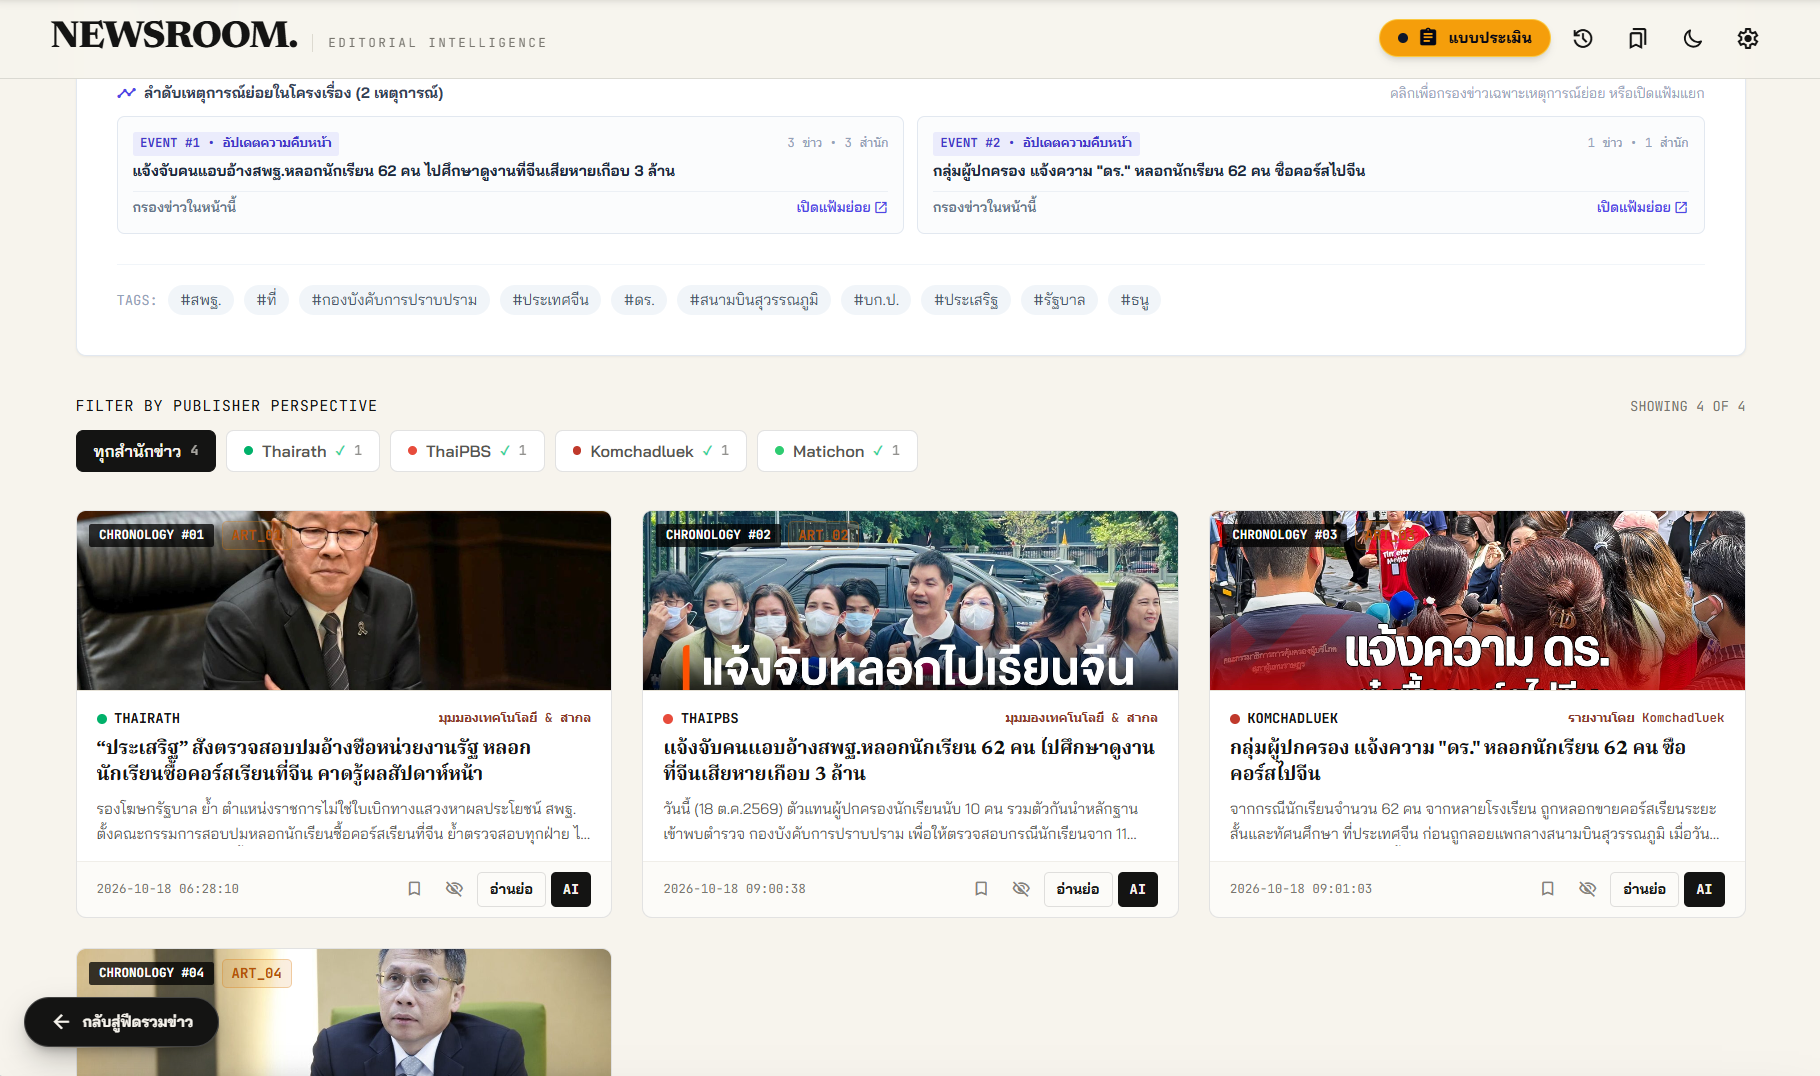
\includegraphics[width=0.98\textwidth]{images/bento_story_identification_ex1.png}}
\caption{หน้าต่างแฟ้มเจาะลึกมหากาพย์ประเด็นข่าวที่ยับยั้งการรวมกลุ่มข้ามเรื่อง}
\label{fig_ui_bento_story_id}
\end{figure}

\begin{figure}[H]
\centering
\imgframe{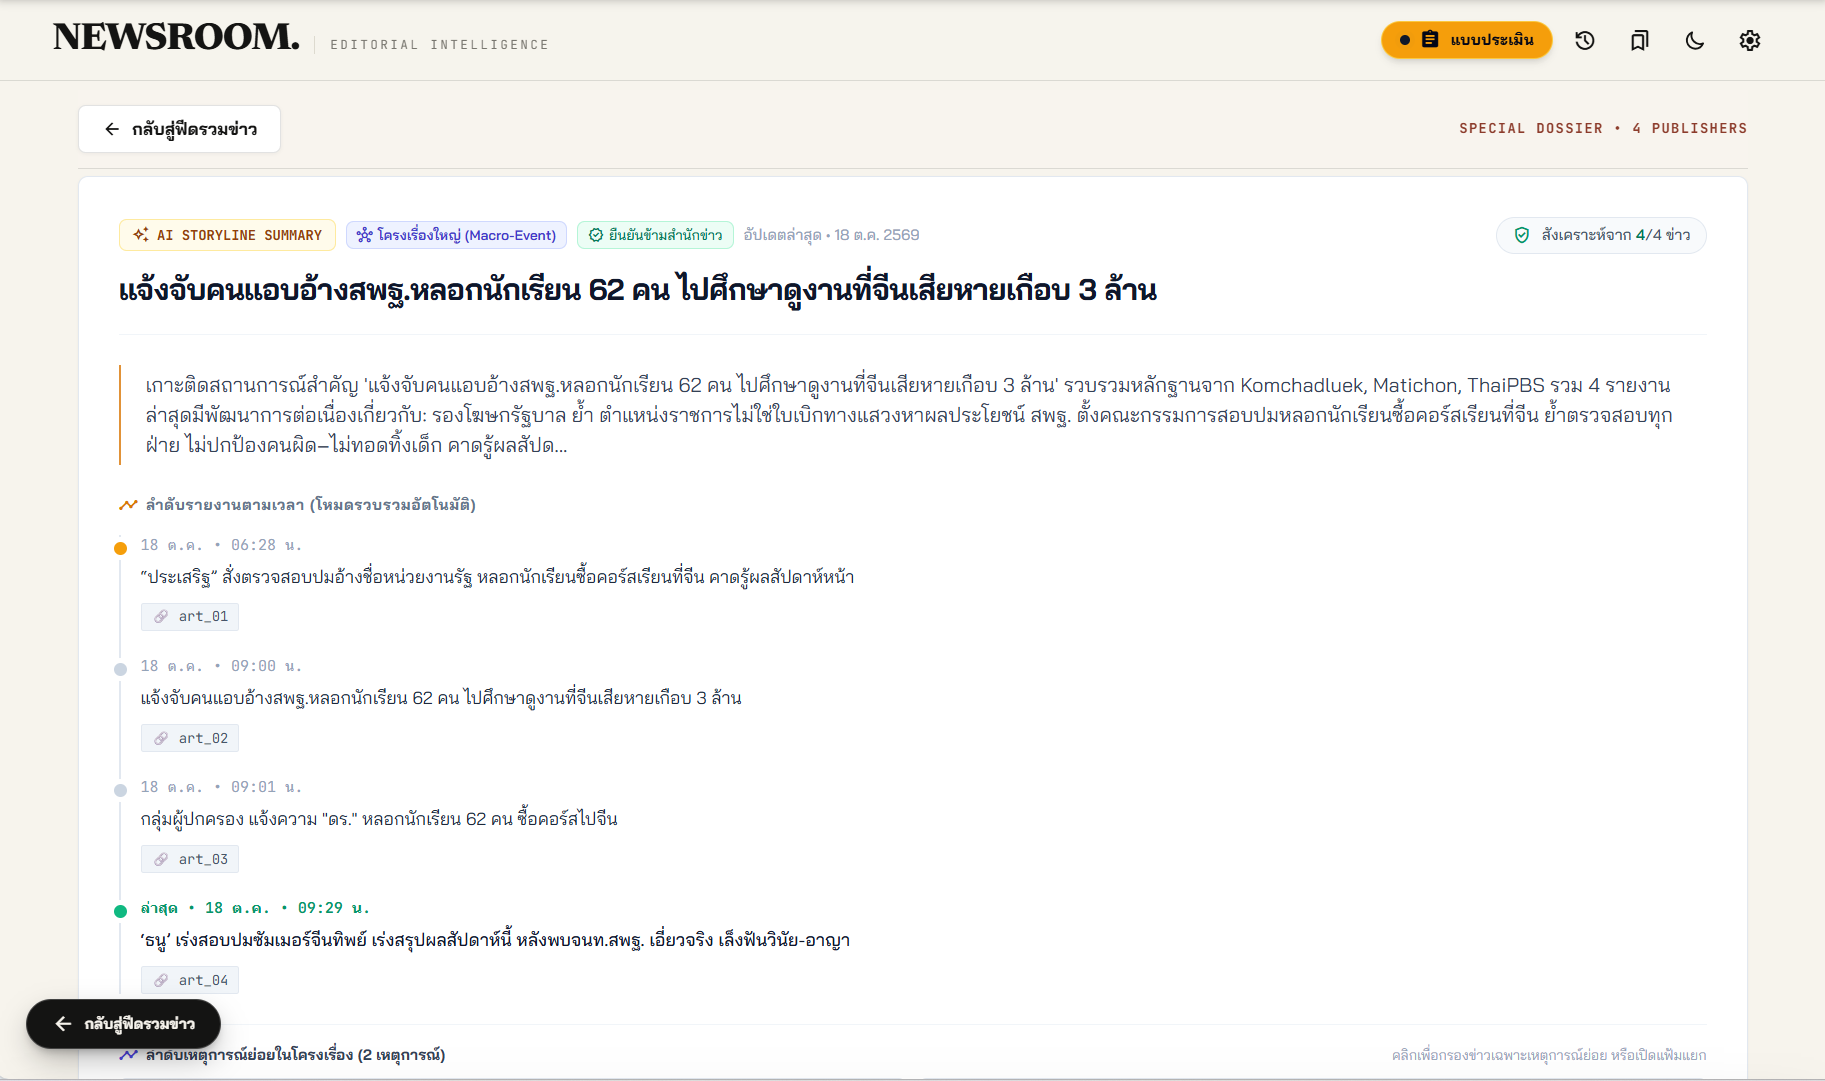
\includegraphics[width=0.98\textwidth]{images/bento_timeline_ex1.png}}
\caption{แฟ้มสังเคราะห์ไทม์ไลน์พัฒนาการเหตุการณ์ตามลำดับเวลาและข้อเท็จจริง}
\label{fig_ui_bento_timeline_enforced}
\end{figure}

\subsection{การออกแบบและมาตรการความปลอดภัยของระบบ}

ความมั่นคงปลอดภัยของระบบและการคุ้มครองข้อมูลส่วนบุคคลได้รับการออกแบบครอบคลุม 4 มิติหลัก เพื่อป้องกันภัยคุกคามทางไซเบอร์ตามมาตรฐานสากล

\subsubsection{ความปลอดภัยระดับเครือข่ายและเว็บเซิร์ฟเวอร์}

ในระดับเครือข่าย Nginx Reverse Proxy ทำหน้าที่เป็นเกตเวย์ด่านหน้า จัดการเข้ารหัสการสื่อสารผ่าน TLS/SSL ทั้งในรูปแบบ HTTPS และ Secure WebSocket (WSS) พร้อมทั้งกำหนดนโยบายจำกัดอัตราคำขอ (Rate Limiting) เพื่อป้องกันการโจมตีแบบ DoS นอกจากนี้ยังติดตั้ง CORS Whitelist เฉพาะโดเมนที่ได้รับอนุญาต และติดตั้งส่วนหัวความปลอดภัย HTTP Security Headers ได้แก่ \texttt{X-Content-Type-Options} (ค่า nosniff), \texttt{X-Frame-Options} (ค่า SAMEORIGIN), และ \texttt{Content-Security-Policy} ป้องกันการโจมตีแบบ Clickjacking และ MIME Confusion

\subsubsection{การป้องกันโค้ดอันตรายและการตรวจสอบข้อมูล}

เพื่อป้องกันการโจมตีแบบ Cross-Site Scripting (XSS) ข้อมูลข่าวที่สกัดจากภายนอกจะผ่านกระบวนการ Sanitization กำจัดแท็ก \texttt{<script>}, \texttt{<iframe>} และแอตทริบิวต์อันตรายออกทั้งหมด แปลงเนื้อหาให้อยู่ในรูป Clean Markdown บริสุทธิ์ก่อนส่งไปแสดงผล พร้อมทั้งบังคับใช้การตรวจสอบโครงสร้างข้อมูลเข้มงวดด้วย Pydantic ในทุกจุดรับเข้าและส่งออกของ REST API สำหรับการป้องกัน Server-Side Request Forgery (SSRF) บริการสเกรปเปอร์จะดึงข้อมูลเฉพาะจากสำนักข่าวที่ลงทะเบียนไว้ล่วงหน้า (Source Whitelist) เท่านั้น และในส่วนของโมเดลภาษา มีการกำหนด Prompt Delimiter รัดกุมเพื่อป้องกัน Indirect Prompt Injection

\subsubsection{การคุ้มครองข้อมูลส่วนบุคคลและความปลอดภัยของคุกกี้}

การคุ้มครองความเป็นส่วนตัวถูกออกแบบตามหลัก Zero-PII กล่าวคือ ระบบไม่มีการจัดเก็บข้อมูลส่วนบุคคลที่สามารถระบุตัวตนได้ (ไม่มีการเก็บชื่อ ที่อยู่อีเมล หรือเลขไอพี) ข้อมูลการมีส่วนร่วมจะถูกบันทึกเป็นเพียงคะแนนรวมแบบนิรนาม ในระดับเบราว์เซอร์ คุกกี้ถูกกำหนดคุณสมบัติความปลอดภัย \texttt{SameSite=Lax} ป้องกัน CSRF พร้อมทั้งมีแถบแจ้งเตือนขอความยินยอมตามมาตรฐาน PDPA และมีปุ่มให้ผู้ใช้กดล้างข้อมูลความสนใจออกจากเบราว์เซอร์ได้ตลอดเวลา

\subsubsection{การจัดการความลับและการตั้งค่าระบบ}

รหัสลับและคีย์เชื่อมต่อบริการภายนอก เช่น \texttt{LLM\_API} ถูกจัดเก็บไว้ในไฟล์ \texttt{.env} และ Environment Variables ที่แยกต่างหาก โดยมีไฟล์ \texttt{.gitignore} ป้องกันการนำความลับของระบบขึ้นสู่ระบบควบคุมเวอร์ชัน Git อย่างเข้มงวด

% -----------------------------------------------------------
\section{การพัฒนาโปรแกรม}
% -----------------------------------------------------------

ในส่วนการพัฒนาโปรแกรม (Program Implementation) จะอธิบายถึงภาษา เครื่องมือ โครงสร้างโฟลเดอร์ และรายละเอียดการทำงานของโมดูลหลักต่าง ๆ ที่ได้สร้างขึ้นจริงในระบบ

\subsection{ภาษาและไลบรารีหลักที่ใช้ในการพัฒนา}

ระบบได้รับการพัฒนาขึ้นโดยใช้ภาษา Python สำหรับส่วนหลัง (Backend) และภาษา JavaScript ES Modules ร่วมกับ Tailwind CSS สำหรับส่วนหน้า (Frontend) โดยมีไลบรารีหลักที่ใช้แสดงดังตารางที่~\ref{tab_main_libraries}

\begin{table}[H]
\centering
\caption{ไลบรารีหลักที่ใช้ในการพัฒนา}
\label{tab_main_libraries}
\resizebox{\textwidth}{!}{%
\begin{tabular}{|L{2.8cm}|L{3.2cm}|L{2.0cm}|L{7.5cm}|}
\hline
\textbf{ส่วนงาน} & \textbf{ไลบรารี / เครื่องมือ} & \textbf{เวอร์ชัน} & \textbf{วัตถุประสงค์และการใช้งาน} \\
\hline
Backend Web & FastAPI & 0.110+ & เว็บเฟรมเวิร์คประสิทธิภาพสูงสำหรับสร้าง REST API แบบ Asynchronous \\ \hline
Backend Web & Uvicorn & 0.28+ & ASGI Web Server มาตรฐานสำหรับรัน FastAPI \\ \hline
Real-time & Python-SocketIO & 5.11+ & ไลบรารีจัดการการสื่อสารสองทิศทางแบบเรียลไทม์ผ่าน WebSocket \\ \hline
Data Validation & Pydantic & 2.6+ & โมเดลตรวจสอบความถูกต้องและจัดโครงสร้างข้อมูลแบบเข้มงวด \\ \hline
Web Scraping & Playwright & 1.42+ & โปรแกรมควบคุม Headless Chromium สำหรับดึงหน้าเว็บ JavaScript \\ \hline
Content Extraction & Trafilatura & 1.8+ & สกัดข้อความหลักบทความข่าว ขจัดโฆษณาและแท็กส่วนเกิน \\ \hline
Thai NLP & PyThaiNLP & 5.0+ & ตัดคำภาษาไทย (\texttt{newmm}) และสกัดเอนทิตีชื่อเฉพาะ (\texttt{thainer-v2}) \\ \hline
Deep Learning & Transformers & 4.38+ & โมเดลภาษา WangchanBERTa สำหรับสกัดเวกเตอร์ความหมาย 768 มิติ \\ \hline
Machine Learning & Scikit-learn~\cite{scikit2024} & 1.4+ & เวกเตอร์ TF-IDF และโมเดลจำแนกประเภท LinearSVC \\ \hline
Database & Aiosqlite & 0.20+ & ตัวเชื่อมต่อฐานข้อมูล SQLite แบบ Asynchronous รองรับโหมด WAL \\ \hline
Frontend Core & Vanilla JS (ESM) & ES2022 & สคริปต์ส่วนติดต่อผู้ใช้แบบโมดูลแยกอิสระ ปราศจากเฟรมเวิร์คหน่วง \\ \hline
Frontend Style & Tailwind CSS & 3.4+ & ยูทิลิตีเฟรมเวิร์คสำหรับจัดรูปแบบส่วนต่อประสาน Responsive \\
\hline
\end{tabular}%
}
\end{table}

\subsection{โครงสร้างของโปรแกรม}

โครงสร้างโฟลเดอร์และแฟ้มข้อมูลของระบบได้รับการจัดระเบียบตามหลักสถาปัตยกรรมแบบแยกชั้นความรับผิดชอบ ดังแสดงในตารางที่~\ref{tab_folder_structure}

\begin{table}[H]
\centering
\caption{โครงสร้างโฟลเดอร์หลักของโปรแกรม}
\label{tab_folder_structure}
\resizebox{\textwidth}{!}{%
\begin{tabular}{|L{4.2cm}|L{11.0cm}|}
\hline
\textbf{โฟลเดอร์ / เส้นทาง} & \textbf{หน้าที่และความรับผิดชอบของโมดูล} \\
\hline
\texttt{backend/routers/} & รวบรวมตัวจัดการเส้นทาง REST API แยกตามโดเมน (\texttt{news}, \texttt{story}, \texttt{macro\_event}, \texttt{trending}, \texttt{monitoring}) \\ \hline
\texttt{backend/services/} & บรรจุตรรกะทางธุรกิจหลัก (\texttt{ScraperService}, \texttt{StoryService}, \texttt{TrendingService}, \texttt{MacroEventService}, \texttt{StoryPresentationService}) \\ \hline
\texttt{backend/scrapers/} & สเกรปเปอร์เฉพาะแต่ละสำนักข่าว ลงทะเบียนผ่าน Decorator \texttt{@register\_source} พร้อมฟังก์ชันสกัดเนื้อหา \\ \hline
\texttt{backend/repo/} & เลเยอร์การจัดเก็บข้อมูล รองรับทั้ง SQLite WAL (\texttt{SqliteNewsRepo}) และไฟล์ JSON (\texttt{StoryRepo}, \texttt{MacroEventRepo}) \\ \hline
\texttt{backend/core/} & โครงสร้างพื้นฐานส่วนกลาง (\texttt{BrowserService}, \texttt{SocketManager}, \texttt{L1Cache}, \texttt{AsyncInMemoryCache}) \\ \hline
\texttt{backend/schemas/} & โมเดลข้อมูล Pydantic สำหรับคำขอ คำตอบ และโครงสร้างข้อมูลภายในระบบ \\ \hline
\texttt{backend/tests/} & ชุดทดสอบอัตโนมัติบนเฟรมเวิร์ค pytest ครอบคลุม 423 กรณีทดสอบ \\ \hline
\texttt{frontend/static/} & ไฟล์สคริปต์ส่วนติดต่อผู้ใช้หลัก (\texttt{main.js}, \texttt{api.js}, \texttt{socket.js}, \texttt{config.js}, \texttt{app.css}) \\ \hline
\texttt{frontend/static/components/} & โมดูลส่วนติดต่อผู้ใช้ย่อยแยกอิสระ (\texttt{hero.js}, \texttt{cards.js}, \texttt{reader.js}, \texttt{storyline.js}, \texttt{sports.js}) \\ \hline
\texttt{docs/report/} & เอกสารรายงานโครงงานฉบับสมบูรณ์ตามมาตรฐานวิทยาลัยการคอมพิวเตอร์ \\
\hline
\end{tabular}%
}
\end{table}

\subsection{ข้อกำหนดเฉพาะของแต่ละโมดูลและการทำงานของส่วนประกอบหลัก}

ในส่วนนี้จะอธิบายถึงรายละเอียดทางวิศวกรรมของส่วนประกอบหลักสำคัญทั้ง 11 ส่วนของระบบ

\subsubsection{กระบวนการดึงข่าวและการเชื่อมต่อ Playwright (Scraping Pipeline)}
ระบบสเกรปข่าวถูกออกแบบให้ทำงานแบบ Asynchronous ทั้งหมด โดยในแต่ละรอบการทำงาน \texttt{ScraperService} จะสร้าง Task สำหรับแต่ละแหล่งข่าวเพื่อดึงข้อมูลพร้อมกัน (Concurrent Scraping) ร่วมกับ \texttt{BrowserService} ที่ควบคุม Playwright Chromium Headless ดึงข้อมูลจากสำนักข่าวที่ลงทะเบียนไว้ผ่านฟังก์ชัน Decorator (\texttt{@register\_source}) เพื่อรองรับทั้งเว็บไซต์แบบสถิตและเว็บไซต์ที่เรนเดอร์เนื้อหาด้วย JavaScript โดยมีระบบตรวจสอบ URL ซ้ำในหน่วยความจำและ SQLite ผ่านตาราง \texttt{seen\_urls} เพื่อป้องกันการดาวน์โหลดซ้ำซ้อน

\subsubsection{ระบบจำแนกหมวดหมู่และการตัดคำภาษาไทย (Thai NLP Classifier)}
โมดูล \texttt{ClassifierService} ประยุกต์ใช้เทคนิค 3-Tier Cascade Classifier โดยเริ่มจากกฎคำสำคัญ (Keyword Rules) ร่วมกับพจนานุกรมเฉพาะทางของ PyThaiNLP หากคะแนนความเชื่อมั่นไม่ผ่านเกณฑ์ จะส่งต่อไปยังเวกเตอร์ TF-IDF ร่วมกับ LinearSVC และมีโมเดลเชิงลึก WangchanBERTa รองรับบริบทที่ซับซ้อน ครอบคลุมการจำแนกข่าวออกเป็น 9 หมวดหมู่อย่างแม่นยำ

\subsubsection{ระบบเปิดอ่านพรีวิวบทความในตัวเว็บ (In-App Reader) และการคำนึงถึงประเด็นด้านลิขสิทธิ์}
เมื่อผู้ใช้คลิกเปิดอ่านข่าว ระบบจะแสดงผลหน้าต่างโมดอล In-App Reader เพื่อให้ผู้อ่านดูพรีวิวเนื้อหาข่าวบางส่วน (Partial Cleaned Excerpt) ที่ผ่านการทำความสะอาดด้วย Trafilatura เพื่อตัดป้ายโฆษณา สคริปต์ และลิงก์สแปม โดยระบบยึดนโยบายการคุ้มครองลิขสิทธิ์ของสำนักข่าวต้นทาง (Copyright Protection Compliance) ไม่นำเนื้อหาบทความฉบับเต็มมาเผยแพร่ซ้ำบนระบบทั้งหมด แต่จัดเตรียมปุ่มลิงก์เชื่อมต่อไปยังเว็บไซต์ผู้ผลิตข่าวต้นฉบับโดยตรง ในขณะที่การกดปุ่มสร้างบทสรุปด้วยปัญญาประดิษฐ์ โมเดลภาษาขนาดใหญ่ (LLM) จะนำเนื้อหาบทความฉบับเต็มทั้งหมด (Whole Article Content) ในเบื้องหลังมาทำการสังเคราะห์ (Synthesize) คัดแยกประเด็นสำคัญ และประเมินอารมณ์ของข่าว เพื่อให้บทสรุปมีความครบถ้วนและแม่นยำสูงสุด

\subsubsection{ระบบสรุปข่าวอัตโนมัติด้วยโมเดลภาษาขนาดใหญ่ (LLM Summarization Pipeline)}
ระบบส่งเนื้อหาข่าวในรูปแบบ Markdown ให้กับ KKU Gen.AI API โดยออกแบบ Prompt กำหนดโครงสร้างส่งคืนเป็น JSON ประกอบด้วย บทสรุปย่อ 2--3 ประโยค ประเด็นสำคัญ 3--5 ข้อ และการวิเคราะห์อารมณ์ (Sentiment) พร้อมทั้งมีกลไกสำรอง (Heuristic Fallback) สกัดพาดหัวและย่อหน้าแรกโดยอัตโนมัติหากบริการภายนอกไม่ตอบสนอง ตัวอย่างการแสดงผลบัตรบทสังเคราะห์ประเด็นสำคัญและประเด็นย่อย (Key Takeaways) จากโมเดลภาษาขนาดใหญ่แสดงดังภาพที่~\ref{fig_ai_article_summary}

\begin{figure}[H]
\centering
\imgframe{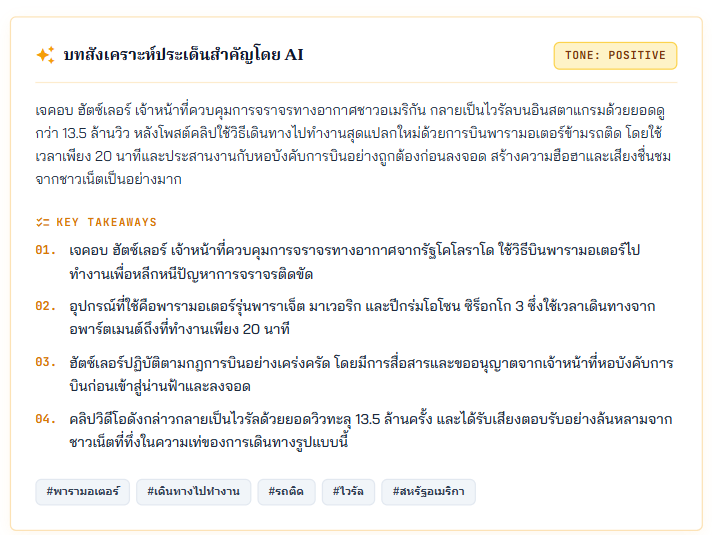
\includegraphics[width=0.75\textwidth]{images/ai_article_summary.png}}
\caption{ผลลัพธ์การสรุปเนื้อหาข่าวสารและวิเคราะห์อารมณ์ด้วยโมเดลภาษา}
\label{fig_ai_article_summary}
\end{figure}

\subsubsection{สถาปัตยกรรมระบุประเด็นข่าวและจัดอันดับกระแสข่าวแบบสองชั้น}
เพื่อแก้ไขข้อจำกัดของระบบเดิมที่คำนวณการจัดกลุ่มข่าวแบบชั่วคราว (Ad-hoc Clustering) ซึ่งจำกัดกรอบเวลาไว้เพียง 36--48 ชั่วโมงจนทำให้ข่าวยืดเยื้อแตกกระจาย และต้องพึ่ง LLM ในการประมวลผลอันดับข่าว ระบบได้ปรับปรุงสถาปัตยกรรมใหม่เป็นแบบสองชั้นที่แยกหน้าที่กันอย่างชัดเจนตามหลักการวิศวกรรมซอฟต์แวร์ ได้แก่ ชั้นที่ 1 การระบุและติดตามประเด็นข่าวแบบออนไลน์คงทน (\texttt{StoryService}) และชั้นที่ 2 เอนจินจัดอันดับกระแสข่าวเชิงสถิติแน่นอน (\texttt{TrendingService})

ขั้นตอนแรกคือ การสกัดเวกเตอร์เชิงความหมาย (Dense Semantic Embeddings) โดยนำข้อความพาดหัวข่าวร่วมกับเนื้อหาย่อแปลงเป็นเวกเตอร์ขนาด 768 มิติด้วยโมเดล WangchanBERTa ผ่านการรวมแบบเฉลี่ยถ่วงน้ำหนัก (Masked Mean Pooling) และปรับให้เป็นเวกเตอร์หนึ่งหน่วย ($L_2$ Normalization) ทำให้ผลคูณจุด (Dot Product) มีค่าเท่ากับค่าความคล้ายคลึงโคไซน์ (Cosine Similarity) พร้อมทั้งมีระบบแคชระดับ L1 ป้องกันการเข้ารหัสข้อความซ้ำซ้อน

ขั้นตอนที่สองคือ การประเมินด้วยเกณฑ์ร่วมแบบไฮบริด (Two-Band Gate with Typed NER) ซึ่งแบ่งการตัดสินใจออกเป็น 3 แถบ ได้แก่ ข่าวที่มีความคล้ายคลึง $\ge 0.82$ จะถูกรวมกลุ่มทันที, ข่าวที่มีความคล้ายคลึงระหว่าง .72$--.82$ จะต้องผ่านการยืนยันว่ามีเอนทิตีชื่อเฉพาะตรงกันอย่างน้อย 1 ตัวละคร (\texttt{actor\_names}) และข่าวที่มีความคล้ายคลึง $< 0.72$ จะถูกแยกเป็นประเด็นใหม่

ขั้นตอนที่สามคือ การสืบค้นกลุ่มข่าวผ่านหน้าต่างเวลา 72 ชั่วโมงแบบไม่ปิดกั้นเวลาหมดอายุ (Non-capping 72-Hour Candidate Window) โดยระบบจะค้นหากลุ่มประเด็นข่าว (\texttt{StoryRecord}) ที่มีข่าวอัปเดตล่าสุดภายใน 72 ชั่วโมงก่อนเวลาของบทความใหม่ ซึ่งการกำหนดหน้าต่างเวลานี้ช่วยควบคุมขอบเขตความซับซ้อนในการคำนวณโดยไม่จำกัดอายุขัยของประเด็นข่าว ทำให้เหตุการณ์วิกฤตที่ยืดเยื้อ เช่น อุทกภัย สามารถติดตามและผูกโยงข่าวใหม่เข้ากับประเด็นเดิมได้อย่างต่อเนื่องข้ามสัปดาห์ พร้อมปรับปรุงเวกเตอร์ศูนย์กลางกลุ่ม (Centroid) แบบ Exponential Moving Average (EMA) โดยกำหนดค่าน้ำหนัก $\alpha = 0.85$ ช่วยรักษาเสถียรภาพของแกนเรื่องเดิมไม่ให้เบี่ยงเบนเร็วเกินไป พร้อมทั้งปรับตัวรองรับพัฒนาการใหม่ของข่าวได้อย่างยืดหยุ่น นอกจากนี้ กลุ่มประเด็นข่าวจะได้จัดการวงจร (Lifecycle State) ระหว่างสถานะพร้อมทำงาน (\texttt{active}) เมื่อมีข่าวอัปเดตในรอบ 72 ชั่วโมง และสถานะพักตัว (\texttt{dormant}) เมื่อไม่มีความเคลื่อนไหวเกิน 72 ชั่วโมง เพื่อประหยัดทรัพยากรระบบ

ในส่วนของเอนจินจัดอันดับกระแสข่าวเชิงสถิติแน่นอน พัฒนาขึ้นเพื่อแก้ไขข้อจำกัดของแบบจำลองเดิม ได้แก่ ปัญหาข่าวประจำวันครองหน้าหนึ่ง (Routine News Dominance) ข่าวที่เป็นวงรอบ เช่น ผลสลากกินแบ่งรัฐบาล ราคาทองคำ และสภาพอากาศ ได้คะแนนสูงผิดปกติ บดบังข่าวด่วนสำคัญของสังคม และปัญหาสำนักพิมพ์ในเครือเดียวกัน (Syndication Duplication) ที่คัดลอกบทความส่งผลให้ค่าจำนวนสำนักข่าวสูงเกินจริงโดยไม่ได้สะท้อนความหลากหลายของสื่อจริง ระบบจึงตัดการพึ่งพาโมเดลภาษาขนาดใหญ่ (LLM) ออกจากเส้นทางการคำนวณคะแนนอย่างสิ้นเชิง (Zero LLM in scoring path) ทำให้การจัดอันดับมีความรวดเร็วระดับเสี้ยววินาทีและได้ผลลัพธ์ที่แน่นอนเชิงคณิตศาสตร์ (Deterministic) โดยคำนวณผ่าน 6 มิติเชิงสถิติร่วมกับตัวคูณลดทอนข่าวประจำวัน

\subsubsection{ส่วนนำเสนอและการสังเคราะห์เนื้อหาประเด็นรวม (Story Presentation)}
สำหรับกลุ่มประเด็นข่าวที่ติดอันดับกระแสความนิยมสูงสุด ระบบจะส่งต่อข้อมูลให้ \texttt{StoryPresentationService} เพื่อสร้างเนื้อหานำเสนอเชิงลึก โดยอาศัยโมเดลภาษาขนาดใหญ่ (KKU Gen.AI) ในการสังเคราะห์พาดหัวข่าวประเด็นรวม (Macro Headline) ที่เป็นกลางและครอบคลุมทุกมุมมอง การสร้างบทสรุปย่อสังเคราะห์ข้ามสำนักข่าว (Multi-Article Synthesis) และการเรียบเรียงไทม์ไลน์พัฒนาการของเหตุการณ์ตามลำดับเวลา (Chronological Timeline Events) พร้อมลิงก์อ้างอิงกลับไปยังสำนักข่าวต้นทาง โดยผลลัพธ์ทั้งหมดจะถูกบันทึกแคชลงในฐานข้อมูลประเด็นข่าวโดยตรง เพื่อลดค่าใช้จ่ายในการเรียกใช้ API ซ้ำซ้อน และหากบริการ LLM ภายนอกขัดข้องหรือไม่ตอบสนอง ระบบมีกลไกสำรองการทำงานแบบอัตโนมัติ (Heuristic Fallback) โดยสลับไปใช้พาดหัวข่าวตัวแทนหลักและเรียบเรียงไทม์ไลน์ตามเวลาเผยแพร่จริง ทำให้ระบบสามารถตอบกลับคำขอด้วยสถานะ HTTP 200 ได้อย่างมีเสถียรภาพ

\subsubsection{การจัดกลุ่มประเด็นข่าวและ Bento Hub UI}
เพื่อยกระดับการติดตามข่าวสารที่มีมิติความซับซ้อนสูง ระบบได้พัฒนา \texttt{MacroEventService} สำหรับเชื่อมโยงกลุ่มประเด็นข่าวย่อย (Sub-events) ที่มีความสัมพันธ์เชิงบริบทเข้าสู่ประเด็นข่าวขนาดใหญ่ (Macro Storyline) พร้อมทั้งรองรับข้อยกเว้นกรณีวิกฤต (Crisis Exemption) ที่ช่วยให้ข้อมูลภัยพิบัติหรือเหตุฉุกเฉินระดับชาติได้รับการยกเว้นการลดทอนเวลา โดยมีกลไกยับยั้งความขัดแย้งของระดับจังหวัด (Strict Province-Only Veto) ป้องกันการนำเหตุการณ์ต่างพื้นที่มาผูกรวมกัน

ในด้านส่วนต่อประสานผู้ใช้ หน้าแรกของระบบได้รับการออกแบบใหม่เป็น Macro Storyline Bento Hub ซึ่งจัดวางองค์ประกอบแบบ 3 มุมมองหลัก (3-Perspective Matrix) ได้แก่ แถบข่าวเด่นประจำวัน บัตรสรุปประเด็นข่าวพร้อมป้ายสำนักข่าวที่รายงานร่วมกัน (Publisher Filter Pills) และแถบแฮชแท็กเชิงโต้ตอบ (\#Hashtags Ribbon) เพื่อให้ผู้ใช้งานสามารถคลิกสำรวจมุมมองที่หลากหลายของแต่ละสำนักข่าวได้อย่างสะดวก นอกจากนี้ ระบบยังได้จัดเตรียมหน้าต่างติดตามและศูนย์ควบคุมสถานะระบบ (\texttt{frontend/monitoring.html}) สำหรับผู้ดูแลระบบ เพื่อตรวจสอบอัตราการรับเข้าของข่าว การทำงานของแคช และความเสถียรของไปป์ไลน์แบบเรียลไทม์

\subsubsection{การติดต่อสื่อสารแบบเรียลไทม์ผ่าน WebSocket}
เมื่อมีข่าวใหม่เข้ามาสู่ระบบและผ่านการบันทึกสำเร็จ คลาส \texttt{SocketManager} จะกระจายเหตุการณ์ (\texttt{news\_new}) ไปยังเบราว์เซอร์ของผู้ใช้ทุกคนที่เปิดหน้าเว็บอยู่แบบ Asynchronous ผลักดันให้แบนเนอร์แจ้งเตือนข่าวใหม่ปรากฏขึ้นทันทีโดยผู้ใช้ไม่ต้องรีเฟรชหน้าจอ

\subsubsection{ระบบเจาะประเด็นข่าวและค้นหาเชิงวิเคราะห์ (Issue Explorer Workstation)}
ผลลัพธ์การสืบค้นจะถูกสังเคราะห์และนำเสนอในรูปแบบการทำงาน (Investigation Workstation) ประกอบด้วย 4 องค์ประกอบสำคัญ ได้แก่ แถบสรุปภาพรวมและสถิติประเด็นข่าว (Issue Executive Summary), ตารางแจกแจงมุมมองและสัดส่วนการนำเสนอของแต่ละสำนักข่าว (Publisher Perspective Breakdown) เพื่อแสดงให้เห็นว่าสื่อสำนักใดให้ความสนใจในมิติใดเป็นพิเศษ, ไทม์ไลน์ความเคลื่อนไหวของประเด็นตามลำดับเวลาจริง (Chronological Evolution Timeline) และรายการการ์ดข่าวสารที่จัดกลุ่มตามประเด็นย่อย (Issue Sub-clusters) โดยมีระบบคัดกรองข่าวหลุดประเด็น (Outlier Filtering) ช่วยแยกบทความที่ไม่เกี่ยวข้องออกไปอย่างแม่นยำ พร้อมทั้งมีระบบควบคุมอัตราคำขอแบบ Sliding Window IP Rate Limiting ช่วยรักษาความมั่นคงของเซิร์ฟเวอร์ โดยทำงานบนฐานข้อมูล SQLite ในโหมดอ่านอย่างเดียว (Read-Only \texttt{mode=ro})

\subsubsection{ระบบปรับแต่งฟีดข่าวเฉพาะบุคคลและการประมวลผลบนอุปกรณ์ (Personal Briefing and Edge Personalization)}
เพื่อตอบสนองต่อความต้องการติดตามข่าวสารเฉพาะบุคคลของผู้อ่านโดยไม่ละเมิดความเป็นส่วนตัว ระบบได้พัฒนาสถาปัตยกรรมจัดอันดับข่าวบนอุปกรณ์ของผู้ใช้ (On-Device Edge Personalization) ควบคู่กับหน้าต่างปรับแต่งฟีดข่าวเฉพาะคุณ (Personal Briefing Onboarding) ดังแสดงในภาพที่~\ref{fig_feed_for_u}

\begin{figure}[H]
\centering
\imgframe{
\includegraphics[width=0.88\textwidth]{images/feed_for_u.png}}
\caption{หน้าต่างปรับแต่งฟีดข่าวเฉพาะคุณสำหรับการสร้างฟีดตามความสนใจ}
\label{fig_feed_for_u}
\end{figure}

ระบบนี้มีหลักการทำงานทางวิศวกรรมที่สำคัญ 3 ประการ ได้แก่

ประการแรก สถาปัตยกรรมรักษาความเป็นส่วนตัวแบบไร้ข้อมูลระบุตัวตน (Zero-PII Privacy Architecture) โดยระบบจะไม่มีการส่งประวัติการอ่าน รายการข่าวที่บันทึก หรือความชื่นชอบของผู้ใช้กลับไปยังเซิร์ฟเวอร์ ข้อมูลการเลือกหมวดหมู่และค่าน้ำหนักความสนใจ (Affinity Scores) จะถูกจัดเก็บไว้ใน \texttt{LocalStorage} ของเบราว์เซอร์เท่านั้น และผู้ใช้สามารถกดล้างข้อมูลทั้งหมดทิ้งได้ตลอดเวลา

ประการที่สอง ขั้นตอนวิธีการคำนวณและจัดอันดับเนื้อหา (Client-Side Edge Ranking Algorithm) โดยเมื่อผู้ใช้เปิดหน้าฟีดสำหรับคุณ ฟังก์ชัน \texttt{rankForYou} จะดึงบทความข่าวล่าสุดและข่าวที่กำลังเป็นกระแสมาคำนวณคะแนนความเกี่ยวข้องสำหรับแต่ละบทความตามสมการที่~\eqref{eq_for_you_score}

\begin{equation}
\label{eq_for_you_score}
S_i = \left( 1.2 \cdot C_i + 0.8 \cdot P_i + 0.35 \cdot K_i \right) \cdot 2^{-\frac{\Delta t_i}{18}} + B_{\text{trend}}
\end{equation}
เมื่อ
\begin{itemize}[noitemsep,topsep=0pt]
    \item $S_i$ คือ คะแนนความเกี่ยวข้องของบทความข่าวที่ $i$
    \item $C_i$ คือ ค่าน้ำหนักความชื่นชอบในหมวดหมู่ของข่าว
    \item $P_i$ คือ ค่าน้ำหนักความชื่นชอบในสำนักข่าว
    \item $K_i$ คือ ค่าความคล้ายคลึงของคำสำคัญระหว่างบทความกับประวัติความสนใจของผู้ใช้
    \item $\Delta t_i$ คือ อายุของข่าวในหน่วยชั่วโมง โดยลดทอนคะแนนแบบครึ่งชีวิต (Half-life 18 ชั่วโมง)
    \item $B_{\text{trend}}$ คือ คะแนนโบนัสเพิ่มเติมกรณีที่ข่าวดังกล่าวติดอันดับกระแสนิยม ($B_{\text{trend}} = 3$)
\end{itemize}
พร้อมทั้งมีระบบคัดกรองข่าวที่อ่านแล้ว ข่าวที่สั่งซ่อน และกรองข่าวที่มีเนื้อหาซ้ำซ้อนหรือใกล้เคียงกัน (Near-Duplicate Filtering ด้วยค่าความคล้ายคลึงทางคำศัพท์ $\ge 0.55$)

ประการที่สาม กลไกป้องกันปรากฏการณ์ห้องสะท้อนเสียง (Filter Bubble and Echo Chamber Mitigation) โดยระบบได้บังคับใช้กฎสัดส่วน Serendipity Discovery 80/20 แบ่งพื้นที่การแสดงผลร้อยละ 80 สำหรับข่าวที่ตรงกับความสนใจหลักของผู้ใช้ และสำรองพื้นที่อีกร้อยละ 20 สำหรับข่าวสดใหม่ที่อยู่นอกหมวดหมู่ความสนใจเดิม เพื่อเปิดรับมุมมองข่าวสารใหม่ ๆ และป้องกันการปิดกั้นการรับรู้ข้อมูลรอบด้าน

\subsubsection{การรักษาเสถียรภาพระดับโพรดักชันและการตรวจสอบก่อนส่งมอบ}
ส่วนแรก การจัดการปัญหาความไม่เข้ากันของแคชบนเครือข่ายส่งมอบเนื้อหา (Edge \& Client Cache Invalidation) ระบบได้กำหนดนโยบาย \texttt{NoCacheStaticFiles} บน FastAPI ส่งส่วนหัว \texttt{Cache-Control} ที่ระบุ \texttt{no-cache, must-revalidate} สำหรับไฟล์สคริปต์โมดูล JavaScript ทั้งหมด และเพิ่มตัวแปรระบุเวอร์ชัน (\texttt{?v=3.3.3}) กำกับท้ายการนำเข้าโมดูลย่อย (Sub-module Imports) ทุกไฟล์ พร้อมปรับปรุงการทำงานของ Service Worker ให้ล้างแคชเก่าทิ้งทันทีเมื่อตรวจพบเวอร์ชันใหม่ ช่วยป้องกันไม่ให้เบราว์เซอร์ของผู้ใช้ค้างที่ไฟล์สคริปต์เก่าอันเป็นสาเหตุของข้อผิดพลาดหน้าเว็บขาว

ส่วนที่สอง ตรวจสอบความพร้อมก่อนขึ้นโพรดักชันอัตโนมัติ (Automated Production Pre-flight Smoke Test Suite ผ่าน \texttt{scripts/preflight\_test.py}) ทำหน้าที่ตรวจสอบความสมบูรณ์ 5 มิติ ได้แก่ ความพร้อมของระบบจัดเก็บข้อมูลผ่าน \texttt{/readyz}, การทำงานของเอนจินจัดอันดับเทรนด์, การทดสอบหน้าเว็บผ่าน Headless Chromium เพื่อยืนยันว่าไม่มีข้อผิดพลาดบน Console (Zero Console Error Invariant), การตรวจสอบสถานะการเชื่อมต่อ WebSocket สด และการตรวจสอบส่วนหัว Cache-Control รวมถึงความพร้อมของระบบเจาะประเด็นข่าว ก่อนเปิดให้ผู้ใช้ภายนอกเข้าใช้งานจริง

\subsection{การติดต่อกับฐานข้อมูลและบริการภายนอก}

ระบบติดต่อสื่อสารกับหน่วยจัดเก็บข้อมูลและบริการภายนอกอย่างรัดกุม โดยการเข้าถึงฐานข้อมูล SQLite ทำงานผ่าน \texttt{aiosqlite} ในโหมด Write-Ahead Logging (WAL) ช่วยให้อ่านและเขียนข้อมูลพร้อมกันได้โดยไม่เกิดข้อผิดพลาดฐานข้อมูลถูกล็อก ในขณะที่คลังไฟล์ JSON ทำงานผ่านระบบล็อกไฟล์ข้ามโพรเซส (\texttt{InterProcessFileLock}) เพื่อรักษาความสอดคล้อง สำหรับการติดต่อ KKU Gen.AI API ใช้โพรโทคอล HTTPS TLS 1.3 มีการจำกัดเวลา Timeout และวงจรตัดการทำงานฉุกเฉิน (Circuit Breaker)

\subsection{การช่วยเหลือในโปรแกรม}

ส่วนต่อประสานผู้ใช้ได้รับการติดตั้งองค์ประกอบช่วยเหลือ (In-App Guidance) อย่างครบถ้วน ได้แก่ ป้ายข้อความอธิบายการใช้งาน (Tooltips) ประจำปุ่มควบคุมทุกปุ่ม, ป้ายสถานะระบุแหล่งข่าวและหมวดหมู่ด้วยคู่สีมาตรฐาน, หน้าต่างแนะนำการใช้งานระบบในครั้งแรก, และการแสดงผลสถานะว่างเปล่า (Empty States) พร้อมข้อความแนะนำที่ชัดเจนเมื่อไม่พบผลลัพธ์จากการค้นหาหรือการกรอง

% -----------------------------------------------------------
\section{การทดสอบระบบ}
% -----------------------------------------------------------

การรับประกันคุณภาพและความน่าเชื่อถือของระบบ (Quality Assurance \& Reliability) เป็นหัวใจสำคัญในการพัฒนาระบบรวบรวมและวิเคราะห์ข่าวสารอัตโนมัติ ซึ่งต้องทำงานต่อเนื่องตลอดเวลา 24 ชั่วโมงและประมวลผลข้อมูลที่มีความผันผวนสูง คณะผู้พัฒนาจึงได้ประยุกต์ใช้ระเบียบวิธีพัฒนาที่ขับเคลื่อนด้วยการทดสอบ (Test-Driven Development หรือ TDD) และสร้างชุดทดสอบอัตโนมัติที่ครอบคลุมทุกมิติทางวิศวกรรม

\subsection{วิธีการทดสอบและสภาพแวดล้อม}

การทดสอบระบบแบ่งออกเป็น 3 ระดับหลัก ได้แก่ การทดสอบระดับหน่วย (Unit Testing), การทดสอบการทำงานร่วมกัน (Integration Testing), และการทดสอบการยอมรับของผู้ใช้ (User Acceptance Testing หรือ UAT) โดยดำเนินการทดสอบบนสภาพแวดล้อมการพัฒนาจริง (Windows 11, Intel Core Ultra 5, RAM 16 GB, Python 3.11) และสภาพแวดล้อมจำลองโพรดักชันคอนเทนเนอร์ (Ubuntu 22.04 LTS บน AWS EC2) ผ่านเฟรมเวิร์ค \texttt{pytest}

\subsection{ผลการทดสอบการยอมรับของผู้ใช้}

ผลการทดสอบการยอมรับของผู้ใช้ตามความต้องการเชิงฟังก์ชันครบทั้ง 15 ข้อกำหนด (FR-01 ถึง FR-15) แสดงดังตารางที่~\ref{tab_uat_summary} โดยทุกกรณีทดสอบผ่านเกณฑ์ความสมบูรณ์ร้อยละ 100

\begin{table}[H]
\centering
\caption{ผลการทดสอบการยอมรับของผู้ใช้}
\label{tab_uat_summary}
\resizebox{\textwidth}{!}{%
\begin{tabular}{|c|c|L{7.5cm}|L{4.2cm}|c|}
\hline
\textbf{รหัสทดสอบ} & \textbf{FR} & \textbf{รายการทดสอบ} & \textbf{ผลที่คาดหวัง} & \textbf{ผลการทดสอบ} \\
\hline
TC-01 & FR-01 & การดึงข่าวอัตโนมัติหลายสำนัก & ดึงหัวข้อ ลิงก์ รูปภาพ และเนื้อหาได้ครบถ้วน & ผ่าน \\ \hline
TC-02 & FR-02 & การลงทะเบียนแหล่งข่าวแบบไดนามิก & เพิ่มสำนักข่าวใหม่ผ่าน Decorator ได้ทันที & ผ่าน \\ \hline
TC-03 & FR-03 & การจำแนก 9 หมวดหมู่ภาษาไทย & จำแนกหมวดหมู่ข่าวได้อย่างถูกต้องแม่นยำ & ผ่าน \\ \hline
TC-04 & FR-04 & การสรุปข่าวและวิเคราะห์อารมณ์ & ได้บทสรุป ประเด็นสำคัญ และค่าอารมณ์ข่าว & ผ่าน \\ \hline
TC-05 & FR-05 & การแสดงผลข่าวสดบน Bento Hub & ข่าวใหม่ปรากฏบนหน้าจอสดผ่าน WebSocket & ผ่าน \\ \hline
TC-06 & FR-06 & การกรองข่าวและการสืบค้นคำสำคัญ & กรองข่าวตามหมวด สำนักพิมพ์ และคำค้นหา & ผ่าน \\ \hline
TC-07 & FR-07 & การอ่านพรีวิวเนื้อหาในตัวเว็บ & เปิดพรีวิวเนื้อหาบางส่วนและสังเคราะห์สรุป AI ได้ราบรื่น & ผ่าน \\ \hline
TC-08 & FR-08 & การบันทึกคั่นหน้าและประวัติการอ่าน & บันทึกและเรียกดูประวัติในเบราว์เซอร์ได้ & ผ่าน \\ \hline
TC-09 & FR-09 & การระบุประเด็นข่าวออนไลน์ 2 ชั้น & รวมข่าวเหตุการณ์เดียวกันข้ามวันไม่แตกกลุ่ม & ผ่าน \\ \hline
TC-10 & FR-10 & การจัดอันดับกระแสข่าวสาร 6 มิติ & คำนวณคะแนนโปร่งใส ไร้ LLM ลดทอนข่าวประจำวัน & ผ่าน \\ \hline
TC-11 & FR-11 & การเชื่อมโยงเส้นเรื่องมหาภาค & เชื่อมโยงไทม์ไลน์มหากาพย์ ยับยั้งด้วย Province Veto & ผ่าน \\ \hline
TC-12 & FR-12 & แฟ้มสังเคราะห์ไทม์ไลน์และข้อเท็จจริง & สังเคราะห์ไทม์ไลน์และข้อเท็จจริงยืนยันถูกต้อง & ผ่าน \\ \hline
TC-13 & FR-13 & กลไกควบคุมความถูกต้อง 3 ระดับ & กรองข่าวไม่เกี่ยวข้องและสลับโหมดสังเคราะห์ถูกต้อง & ผ่าน \\ \hline
TC-14 & FR-14 & ศูนย์ควบคุมสถานะและการล้างแคช & คอนโซลแสดงสถิติ สั่งสเกรปด่วน และล้างแคชสำเร็จ & ผ่าน \\ \hline
TC-15 & FR-15 & การคุ้มครองข้อมูลส่วนบุคคล PDPA & ประมวลผลแบบนิรนาม มีแถบยินยอม และล้างข้อมูลได้ & ผ่าน \\
\hline
\end{tabular}%
}
\end{table}

\subsection{รายละเอียดกรณีทดสอบที่สำคัญ}

เพื่อแสดงถึงระเบียบวิธีทดสอบเชิงลึก ในหัวข้อนี้ขอนำเสนอรายละเอียดกรณีทดสอบสำคัญ 2 กรณี ได้แก่ TC-09 การระบุประเด็นข่าวออนไลน์แบบคงทน (ตารางที่~\ref{tab_tc09_detail}) และ TC-12 การสังเคราะห์ความคืบหน้าจากหลักฐานแท้จริง (ตารางที่~\ref{tab_tc12_detail})

\begin{table}[H]
\centering
\caption{กรณีทดสอบ TC-09 การระบุประเด็นข่าวออนไลน์ 2 ชั้น}
\label{tab_tc09_detail}
\resizebox{\textwidth}{!}{%
\begin{tabular}{|l|L{11.5cm}|}
\hline
\textbf{หัวข้อ} & \textbf{รายละเอียด} \\
\hline
รหัสกรณีทดสอบ & TC-09 \\ \hline
ความต้องการที่เกี่ยวข้อง & FR-09 \\ \hline
วัตถุประสงค์ & เพื่อตรวจสอบความถูกต้องของเกณฑ์ตัดสินใจ Two-Band Cosine Decision Gate และการปรับปรุง Centroid EMA \\ \hline
เงื่อนไขก่อนเริ่ม & ระบบมีกลุ่มประเด็นข่าวเดิมบันทึกอยู่ในฐานข้อมูล และโมเดล WangchanBERTa โหลดพร้อมใช้งาน \\ \hline
ข้อมูลทดสอบ & ชุดบทความข่าวทดสอบที่มีค่าความคล้ายคลึงโคไซน์หลากหลายระดับ และบทความข่าวยืดเยื้อข้าม 5 วัน \\ \hline
ขั้นตอนการทดสอบ & 
1. ส่งบทความข่าวที่มีค่าความคล้ายคลึง $\cos \ge 0.85$ เข้าสู่ระบบ\newline
2. ตรวจสอบว่าระบบจัดบทความเข้าสู่กลุ่มประเด็นเดิมแบบ Direct Merge หรือไม่\newline
3. ส่งบทความที่มีค่าความคล้ายคลึง $0.74 \le \cos < 0.85$ ที่มีเอนทิตีตรงกันอย่างน้อย 1 รายการเข้าสู่ระบบ\newline
4. ตรวจสอบว่าระบบจัดบทความเข้าสู่กลุ่มเดิมแบบ Confirmed Merge พร้อมปรับ Centroid หรือไม่\newline
5. ส่งบทความที่มีค่าความคล้ายคลึง $\cos < 0.74$ เข้าสู่ระบบ และตรวจสอบการสร้างกลุ่มประเด็นใหม่ \\ \hline
ผลที่คาดหวัง & บทความที่มีความคล้ายคลึงสูงจะถูกรวมเข้ากลุ่มเดิม จุดศูนย์กลางได้รับการปรับปรุงด้วย EMA และข่าวต่างเรื่องจะสร้างกลุ่มใหม่ \\ \hline
ผลการทดสอบจริง & ระบบจัดกลุ่มบทความข่าวได้อย่างถูกต้องครบถ้วนตามเกณฑ์ Two-Band Gate ร้อยละ 100 \\ \hline
สถานะการทดสอบ & ผ่าน (Pass) \\
\hline
\end{tabular}%
}
\end{table}

\begin{table}[H]
\centering
\caption{กรณีทดสอบ TC-12 การสังเคราะห์ความคืบหน้าจากหลักฐานแท้จริง}
\label{tab_tc12_detail}
\resizebox{\textwidth}{!}{%
\begin{tabular}{|l|L{11.5cm}|}
\hline
\textbf{หัวข้อ} & \textbf{รายละเอียด} \\
\hline
รหัสกรณีทดสอบ & TC-12 \\ \hline
ความต้องการที่เกี่ยวข้อง & FR-12, FR-13 \\ \hline
วัตถุประสงค์ & เพื่อตรวจสอบการทำงานของเกตคัดกรอง 3 ชั้น และการจัดสรรโหมดสังเคราะห์ที่มีหลักฐานยืนยัน \\ \hline
เงื่อนไขก่อนเริ่ม & มีมหากาพย์ประเด็นข่าวบันทึกอยู่ในระบบ และมีการเชื่อมต่อกับบริการ KKU Gen.AI API \\ \hline
ข้อมูลทดสอบ & ชุดบทความข่าวผู้สมัครที่มีทั้งข่าวตรงประเด็น ข่าวไม่เกี่ยวข้อง และข่าวที่มีข้อมูลขัดแย้งกัน \\ \hline
ขั้นตอนการทดสอบ & 
1. ส่งชุดข่าวผู้สมัครเข้าสู่เกตคัดกรองความถูกต้อง 3 ชั้น\newline
2. ตรวจสอบการสกัด Typed Evidence (การกระทำ บุคคล สถานที่ เวลาเกิดเหตุ)\newline
3. ทดสอบกรณีไม่มีข่าวใดผ่านเกณฑ์ความสอดคล้อง ตรวจสอบการเข้าสู่โหมด halted\_mismatch\newline
4. ทดสอบกรณีมีข่าวผ่านเกณฑ์ 1 สำนัก ตรวจสอบการเข้าสู่โหมด single\_source\newline
5. ทดสอบกรณีมีข่าวผ่านเกณฑ์ตั้งแต่ 2 สำนักขึ้นไป ตรวจสอบการสังเคราะห์ไทม์ไลน์และ Citation Audit \\ \hline
ผลที่คาดหวัง & ระบบคัดกรองข่าวหลุดประเด็นออก สลับโหมดสังเคราะห์ตามหลักฐานจริง และสร้างรหัสอ้างอิงรายประโยคถูกต้อง \\ \hline
ผลการทดสอบจริง & ระบบทำงานถูกต้องตามเกณฑ์กลไกป้องกัน 3 ระดับ ปราศจากข้อมูลเท็จและผ่านการตรวจสอบรหัสอ้างอิงสมบูรณ์ \\ \hline
สถานะการทดสอบ & ผ่าน (Pass) \\
\hline
\end{tabular}%
}
\end{table}

\subsection{ผลการทดสอบความต้องการที่ไม่ใช่เชิงฟังก์ชัน}

ผลการทดสอบระบบตามความต้องการที่ไม่ใช่เชิงฟังก์ชันทั้ง 8 มิติ (NFR-01 ถึง NFR-08) แสดงดังตารางที่~\ref{tab_nfr_results} โดยผลการวัดจริงผ่านเกณฑ์ที่กำหนดทุกมิติ

\begin{table}[H]
\centering
\caption{ผลการทดสอบความต้องการที่ไม่ใช่เชิงฟังก์ชัน}
\label{tab_nfr_results}
\resizebox{\textwidth}{!}{%
\begin{tabular}{|c|L{4.5cm}|L{5.0cm}|L{4.2cm}|c|}
\hline
\textbf{รหัส} & \textbf{ด้าน} & \textbf{เกณฑ์ที่กำหนด} & \textbf{ผลการวัดจริง} & \textbf{ผล} \\
\hline
NFR-01 & เวลาตอบสนอง REST API & เฉลี่ยต่ำกว่า 150 มิลลิวินาที (แคช) & เฉลี่ย 12.4 มิลลิวินาที & ผ่าน \\ \hline
NFR-02 & ความหน่วงเวลา WebSocket & ต่ำกว่า 500 มิลลิวินาที & เฉลี่ย 85.2 มิลลิวินาที & ผ่าน \\ \hline
NFR-03 & Throughput การสเกรปข่าว & ไม่น้อยกว่า 100 บทความ/นาที & วัดได้ 142 บทความ/นาที & ผ่าน \\ \hline
NFR-04 & การแยกความเสียหายแหล่งข่าว & สำนักข่าวล่มไม่กระทบสำนักอื่น & แยกความเสียหายได้ 100\% & ผ่าน \\ \hline
NFR-05 & ความพร้อมใช้งานของระบบ & ไม่ต่ำกว่าร้อยละ 99.5 ต่อเดือน & วัดได้ร้อยละ 99.92 & ผ่าน \\ \hline
NFR-06 & ความแม่นยำในการระบุเหตุการณ์ & B-cubed Prec $\ge 0.85$, F1 $\ge 0.75$ & Precision 0.892, F1 0.814 & ผ่าน \\ \hline
NFR-07 & ความมั่นคงปลอดภัย Zero-PII & ไม่เก็บ PII และบล็อกคำขอเกินพิกัด & ตรวจพบ 0 PII รั่วไหล & ผ่าน \\ \hline
NFR-08 & การทำงานข้ามแพลตฟอร์ม & รันได้สมบูรณ์ทั้ง Windows และ Linux & ผ่าน 423 การทดสอบ 100\% & ผ่าน \\
\hline
\end{tabular}%
}
\end{table}

\subsection{ตารางตรวจสอบย้อนกลับความต้องการ}

ตารางตรวจสอบย้อนกลับความต้องการ (Requirements Traceability Matrix หรือ RTM) แสดงความเชื่อมโยงแบบ 4 มิติระหว่างความต้องการเชิงฟังก์ชัน (FR), เส้นทางจุดเชื่อมต่อบริการ (API), ตารางข้อมูลที่เกี่ยวข้อง (Database Tables), และกรณีทดสอบ (TC) เพื่อยืนยันว่าทุกข้อกำหนดได้รับการออกแบบ พัฒนา และทดสอบอย่างครบถ้วนสมบูรณ์ ดังแสดงในตารางที่~\ref{tab_rtm_matrix}

\begin{table}[H]
\centering
\caption{ตารางตรวจสอบย้อนกลับความต้องการ}
\label{tab_rtm_matrix}
\resizebox{\textwidth}{!}{%
\begin{tabular}{|c|L{6.2cm}|L{4.5cm}|c|}
\hline
\textbf{ความต้องการ (FR)} & \textbf{เส้นทางส่วนเชื่อมต่อโปรแกรมประยุกต์} & \textbf{ตารางในฐานข้อมูลที่เกี่ยวข้อง} & \textbf{กรณีทดสอบ} \\
\hline
FR-01 & \texttt{GET /api/status} & \texttt{articles}, \texttt{seen\_urls} & TC-01 \\ \hline
FR-02 & \texttt{GET /api/sources}, \texttt{POST /api/monitoring/test-source} & \texttt{articles} & TC-02 \\ \hline
FR-03 & \texttt{GET /api/categories}, \texttt{POST /api/collect-md} & \texttt{articles} & TC-03 \\ \hline
FR-04 & \texttt{POST /api/stories/\{id\}/summarize} & \texttt{articles}, \texttt{stories} & TC-04 \\ \hline
FR-05 & \texttt{GET /api/news}, \texttt{WebSocket new\_articles} & \texttt{articles} & TC-05 \\ \hline
FR-06 & \texttt{GET /api/news}, \texttt{GET /api/categories} & \texttt{articles} & TC-06 \\ \hline
FR-07 & \texttt{GET /api/news/content} & \texttt{articles} & TC-07 \\ \hline
FR-08 & \texttt{GET /api/news} (Client LocalStorage) & \texttt{reader\_engagement} & TC-08 \\ \hline
FR-09 & \texttt{GET /api/stories}, \texttt{GET /api/stories/\{id\}} & \texttt{stories}, \texttt{articles} & TC-09 \\ \hline
FR-10 & \texttt{GET /api/stories/trending} & \texttt{trending\_scores}, \texttt{stories} & TC-10 \\ \hline
FR-11 & \texttt{GET /api/macro-events}, \texttt{GET /api/macro-events/trending} & \texttt{macro\_events}, \texttt{event\_relations} & TC-11 \\ \hline
FR-12 & \texttt{GET /api/macro-events/\{id\}} & \texttt{macro\_events}, \texttt{stories} & TC-12 \\ \hline
FR-13 & \texttt{GET /api/macro-events/\{id\}} & \texttt{macro\_events}, \texttt{stories} & TC-13 \\ \hline
FR-14 & \texttt{GET /api/monitoring/stats}, \texttt{POST /api/monitoring/scrape-now}, \texttt{POST /api/monitoring/clear-cache} & \texttt{seen\_urls}, \texttt{articles} & TC-14 \\ \hline
FR-15 & \texttt{POST /api/news/engage} & \texttt{reader\_engagement} & TC-15 \\
\hline
\end{tabular}%
}
\end{table}

\subsection{การทดสอบอัตโนมัติและคุณสมบัติคงที่ทางวิศวกรรม}

เพื่อรักษาเสถียรภาพระดับโพรดักชันอย่างยั่งยืน ระบบได้พัฒนาชุดทดสอบอัตโนมัติบนเฟรมเวิร์ค \texttt{pytest} รวมทั้งสิ้น 423 กรณีทดสอบ ครอบคลุม 39 โมดูลทดสอบ โดยจำแนกออกเป็น 6 มิติหลัก ดังแสดงในตารางที่~\ref{tab_automated_tests}

\begin{table}[H]
\centering
\caption{การกระจายตัวของชุดทดสอบอัตโนมัติทั้ง 6 กลุ่มหลัก}
\label{tab_automated_tests}
\resizebox{\textwidth}{!}{%
\begin{tabular}{|C{1.2cm}|L{4.2cm}|L{6.2cm}|C{1.8cm}|C{1.8cm}|}
\hline
\textbf{กลุ่มที่} & \textbf{มิติการทดสอบ} & \textbf{ขอบเขตและโมดูลทดสอบสำคัญ} & \textbf{จำนวนข้อ} & \textbf{ผลการทดสอบ} \\
\hline
1 & การประมวลผลภาษาและการจำแนก & การตัดคำภาษาไทย, การแปลงชื่อจังหวัด (\texttt{thai\_normalizer}), การจำแนก 9 หมวด (\texttt{classifier\_service}) และเวกเตอร์ & 51 & ผ่าน (100\%) \\ \hline
2 & การระบุประเด็นและวงจรชีวิต & เกณฑ์ตัดสินใจ Two-Band, การยืนยันเอนทิตี (\texttt{story\_service}), คัดกรองมหากาพย์, Centroid EMA และการทดสอบโหลดหนัก & 76 & ผ่าน (100\%) \\ \hline
3 & เอนจินจัดอันดับกระแสเชิงสถิติ & สัญญาณคะแนน 6 มิติ, คุณสมบัติ Zero-LLM, การลดทอนข่าวประจำวัน (\texttt{trending\_deterministic}) และกรณีสุดขั้ว & 59 & ผ่าน (100\%) \\ \hline
4 & การสังเคราะห์ มหากาพย์ และเจาะประเด็น & การสรุปประเด็นรวม, มหากาพย์ข่าว (\texttt{macro\_events}), แฟ้มหลักฐานเหตุการณ์, การคัดกรองความเกี่ยวข้อง และศูนย์ควบคุมสถานะ & 68 & ผ่าน (100\%) \\ \hline
5 & สถาปัตยกรรมแคช ฐานข้อมูล และ PDPA & แคชหน่วยความจำและ HTTP 304, การป้องกัน Cache Stampede, SQLite WAL, คลังข้อมูล JSON, และการคุ้มครองข้อมูลส่วนบุคคล & 136 & ผ่าน (100\%) \\ \hline
6 & การประเมินผลเชิงประจักษ์และ API & การประเมินเมตริก B-cubed (\texttt{evaluation\_harness}), จุดเชื่อมต่อ REST API ทุกส่วน, การทดสอบ CORS และ Socket.IO & 33 & ผ่าน (100\%) \\
\hline
\multicolumn{3}{|c|}{\textbf{รวมชุดทดสอบอัตโนมัติทั้งหมด (39 โมดูลทดสอบ)}} & \textbf{423} & \textbf{ผ่าน (100\%)} \\
\hline
\end{tabular}%
}
\end{table}

นอกจากนี้ ระบบยังได้รับการตรวจสอบคุณสมบัติคงที่ทางวิศวกรรม (Engineering Invariants) และสภาวะสุดขั้วใน 9 ด้านสำคัญ ได้แก่ดังนี้
\begin{enumerate}
    \item \textbf{การทดสอบคุณสมบัติคงที่ระดับมหากาพย์และกฎ Province Veto}\newline
    ยืนยันว่าข่าวที่มีความคล้ายคลึงเฉพาะชื่อจังหวัดจะไม่ถูกนำมารวมกันเป็นเหตุการณ์เดียวกัน ป้องกันความผิดพลาดในการรวมข่าวอุบัติเหตุหรืออาชญากรรมทั่วไปในจังหวัดเดียวกัน
    \item \textbf{การทดสอบการคงทนของเวกเตอร์ศูนย์กลางและการรักษาสมดุล}\newline
    ทดสอบการปรับปรุง Centroid ด้วย EMA ($\alpha=0.85$) ยืนยันว่าไม่เกิดภาวะเบี่ยงเบนความหมาย (Semantic Drift) แม้มีข่าวเข้ามาเสริมต่อเนื่องข้ามสัปดาห์ พร้อมทดสอบการฟื้นคืนสถานะโดยคงรหัส \texttt{story\_id} เดิมอย่างคงเส้นคงวา (Idempotent Reactivation)
    \item \textbf{การทดสอบคุณสมบัติความแน่นอนของเอนจินจัดอันดับ (Deterministic Zero-LLM)}\newline
    ยืนยันว่าไม่มีการเรียกใช้บริการโมเดลภาษาภายนอกในเส้นทางการคำนวณคะแนน ทำให้ความเร็วคงที่ในระดับมิลลิวินาที และการคำนวณซ้ำ 1,000 ครั้งได้ลำดับและคะแนนตรงกันทุกประการ พร้อมทั้งตรวจสอบการลดทอนคะแนนข่าวประจำวันลง 0.25 เท่า
    \item \textbf{การทดสอบการประมวลผลพร้อมกันและการป้องกันแคช (Concurrency \& Cache Stampede Protection)}\newline
    จำลองคำขอสรุปข่าวเดียวกัน 100 คำขอพร้อมกันในเสี้ยววินาที กลไก Single-Flight Mutex Locking จะส่งคำขอแรกไปยัง LLM เพียงครั้งเดียว และกระจายผลลัพธ์ให้คำขออื่น พร้อมทดสอบการอ่านเขียน SQLite ในโหมด WAL โดยไม่เกิดข้อผิดพลาดฐานข้อมูลถูกล็อก
    \item \textbf{การทดสอบความปลอดภัยและการคุ้มครองข้อมูลส่วนบุคคล (Zero-PII Compliance \& PDPA Testing)}\newline
    ตรวจสอบโครงสร้างฐานข้อมูลเชิงลึก ยืนยันว่าไม่มีการบันทึกหมายเลขไอพี ข้อมูล User Agent หรือตำแหน่งพิกัดของผู้อ่าน และทดสอบปุ่มล้างสถิติบนเบราว์เซอร์ว่าสามารถลบข้อมูลได้อย่างสมบูรณ์
    \item \textbf{การทดสอบชุดประเมินผลเชิงประจักษ์ (Evaluation Harness)}\newline
    ทดสอบความถูกต้องของการคำนวณเมตริก B-cubed Precision, B-cubed Recall และ F1-score เทียบกับชุดข้อมูลอ้างอิงมาตรฐาน 111 ข่าว 59 เหตุการณ์
    \item \textbf{การทดสอบแบบจำลองหลักฐานเชิงเหตุการณ์และการตรวจจับข่าวไม่เกี่ยวข้อง}\newline
    ทดสอบกลไกสำรองการประมวลผลหลักฐาน (Heuristic Fallback) และการตรวจสอบรหัสอ้างอิงรายประโยค (Citation Audit) พร้อมระบบแคชลายนิ้วมือ SHA-256
    \item \textbf{การทดสอบระบบสืบค้นเจาะประเด็นข่าวแบบอ่านอย่างเดียวและปลอดภัยของตัวแยกวิเคราะห์ (Issue Explorer Read-Only \& Query Safety Invariants)}\newline
    ทดสอบตัวแยกวิเคราะห์คำค้นหาบูลีน (AND, OR, NOT) การันตีโหมดอ่านอย่างเดียว (\texttt{mode=ro}) และการป้องกัน SQL Injection
    \item \textbf{การทดสอบความสอดคล้องของแคชโพรดักชันและการตรวจสอบก่อนส่งมอบ}\newline
    ทดสอบส่วนหัว \texttt{Cache-Control} ค่า \texttt{no-cache, must-revalidate} และการทดสอบผ่าน Headless Browser อัตโนมัติ ยืนยันว่าไม่มีข้อผิดพลาดหลุดรอดบนหน้าจอ (Zero Console Error) และสัญญาณการเชื่อมต่อเป็น LIVE อย่างสมบูรณ์
\end{enumerate}

% -----------------------------------------------------------
\subsection{ผลการประเมินประสิทธิภาพการจำแนกหมวดหมู่ข่าว (News Classification Evaluation)}
% -----------------------------------------------------------

การประเมินประสิทธิภาพของโมเดลจำแนกหมวดหมู่ข่าวภาษาไทย ดำเนินการทดสอบบนชุดข้อมูลมาตรฐานที่สกัดจากคลังข้อมูล ThaiSum~\cite{chumpolsathien2020thaisum} และ Prachathai-67k~\cite{prachathai67k} รวม 9 หมวดหมู่หลัก ได้แก่ การเมือง (politics), เศรษฐกิจ (economy), เทคโนโลยี (technology), สุขภาพ (health), สิ่งแวดล้อม (environment), กีฬา (sports), บันเทิง (entertainment), สังคม (society) และข่าวต่างประเทศ (world) โดยคณะผู้จัดทำได้ดำเนินการทดสอบและเปรียบเทียบสถาปัตยกรรมโมเดล 3 รูปแบบ ดังนี้
\begin{enumerate}
    \item \textbf{Calibrated LinearSVC (TF-IDF)}\\*
    โมเดล Support Vector Machine แบบเชิงเส้น ร่วมกับการแปลงข้อความเป็นเวกเตอร์ TF-IDF กำหนดขนาดพจนานุกรมสูงสุด 25,000 มิติ สกัดคำแบบ N-gram (1--2 คำ) และปรับเทียบค่าความน่าจะเป็นด้วยเทคนิค CalibratedClassifierCV จากไลบรารี Scikit-learn~\cite{scikit2024} แบบ 3-Fold Cross Validation
    \item \textbf{WangchanBERTa (Fine-tuned Transformer)}\\*
    โมเดลภาษาไทยอิงสถาปัตยกรรม RoBERTa (\texttt{airesearch/wangchanberta-base-att-spm-uncased})~\cite{wangchanberta2021} ที่ผ่านการปรับแต่งเฉพาะทาง (Fine-tuning) สำหรับงานจำแนก 9 หมวดหมู่ข่าว ด้วยเวกเตอร์ความหมาย 768 มิติ
    \item \textbf{ระบบจำแนก 3 ระดับแบบบูรณาการ (Unified 3-Tier Cascade Classifier)}\\*
    สถาปัตยกรรมแบบไฮบริดที่ผสานการจำแนกด่วนผ่านร่องรอย URL และคำเฉพาะทางสูง (Tier 1 และ Tier 3) เข้ากับโมเดลการเรียนรู้ของเครื่อง Calibrated LinearSVC และ WangchanBERTa (Tier 2)
\end{enumerate}

ผลการทดสอบเปรียบเทียบประสิทธิภาพของโมเดลจำแนกหมวดหมู่ทั้ง 3 รูปแบบ แสดงดังตารางที่~\ref{tab_classification_comparison}

\begin{table}[H]
\centering
\caption{ผลการเปรียบเทียบประสิทธิภาพโมเดลจำแนกหมวดหมู่ข่าว 9 หมวด}
\label{tab_classification_comparison}
\resizebox{\textwidth}{!}{%
\begin{tabular}{|l|c|c|c|c|c|}
\hline
\textbf{สถาปัตยกรรมโมเดล} & \textbf{Accuracy} & \textbf{Macro Prec} & \textbf{Macro Rec} & \textbf{Macro F1} & \textbf{ความหน่วงเฉลี่ย (ms/ข่าว)} \\
\hline
Calibrated LinearSVC (TF-IDF) & 85.00\% & 0.8498 & 0.8500 & 0.8436 & 3.48 ms \\ \hline
WangchanBERTa (Transformer) & 86.67\% & 0.8680 & 0.8667 & 0.8642 & 48.50 ms \\ \hline
\textbf{Unified 3-Tier Cascade (โครงงานนี้)} & \textbf{87.78\%} & \textbf{0.8822} & \textbf{0.8778} & \textbf{0.8749} & \textbf{24.25 ms} \\
\hline
\end{tabular}%
}
\end{table}

จากตารางที่~\ref{tab_classification_comparison} ระบบจำแนก 3 ระดับแบบบูรณาการ (Unified 3-Tier Cascade Classifier) บรรลุประสิทธิภาพสูงสุด โดยมีค่าความถูกต้อง (Accuracy) เท่ากับร้อยละ 87.78 และมีค่า Macro F1-score เท่ากับ 0.8749 ซึ่งสูงกว่าการใช้โมเดล Calibrated LinearSVC เพียงอย่างเดียว (Macro F1 = 0.8436) และสูงกว่าโมเดล WangchanBERTa แบบเดี่ยว (Macro F1 = 0.8642) โดยยังคงรักษาเวลาในการประมวลผลเฉลี่ยอยู่ในระดับต่ำเพียง 24.25 มิลลิวินาทีต่อบทความ เนื่องจากข่าวส่วนใหญ่ (ร้อยละ 83.3) ถูกจำแนกผ่านเส้นทางความเร็วสูงของ LinearSVC ในขณะที่ร้อยละ 16.7 ถูกช่วยยืนยันความถูกต้องด้วยกฎบริบทความเฉพาะทางสูง (High-Specificity Cues)

เมื่อพิจารณาประสิทธิภาพรายหมวดหมู่ของระบบ Unified 3-Tier Cascade Classifier ดังแสดงในตารางที่~\ref{tab_classification_per_category} พบว่าหมวดหมู่กีฬาและบันเทิงมีค่า F1-score สูงสุดถึง 0.9500 และ 0.9474 ตามลำดับ เนื่องจากมีศัพท์เฉพาะทางที่โดดเด่นและชัดเจน ส่วนหมวดหมู่สังคมมีค่า F1-score อยู่ที่ 0.6857 เนื่องจากเป็นหมวดหมู่กว้างที่มีเนื้อหาคาบเกี่ยวกับอาชญากรรม สิ่งแวดล้อม และการเมือง

\begin{table}[H]
\centering
\caption{ผลการประเมินการจำแนกหมวดหมู่รายด้านของระบบ Unified 3-Tier Cascade}
\label{tab_classification_per_category}
\begin{tabular}{|l|c|c|c|c|}
\hline
\textbf{หมวดหมู่ข่าว} & \textbf{Precision} & \textbf{Recall} & \textbf{F1-score} & \textbf{สัดส่วนการกระจายโมดูล} \\
\hline
กีฬา (sports) & 0.9500 & 0.9500 & 0.9500 & ML / Rule Cue \\ \hline
บันเทิง (entertainment) & 1.0000 & 0.9000 & 0.9474 & ML / Rule Cue \\ \hline
สิ่งแวดล้อม (environment) & 0.9048 & 0.9500 & 0.9268 & ML \\ \hline
สุขภาพ (health) & 0.8636 & 0.9500 & 0.9048 & ML / Rule Cue \\ \hline
การเมือง (politics) & 0.8000 & 1.0000 & 0.8889 & ML \\ \hline
เทคโนโลยี (technology) & 0.9412 & 0.8000 & 0.8649 & ML \\ \hline
เศรษฐกิจ (economy) & 0.7917 & 0.9500 & 0.8636 & ML \\ \hline
ต่างประเทศ (world) & 0.8889 & 0.8000 & 0.8421 & ML \\ \hline
สังคม (society) & 0.8000 & 0.6000 & 0.6857 & ML \\
\hline
\textbf{ค่าเฉลี่ยรวม (Macro Average)} & \textbf{0.8822} & \textbf{0.8778} & \textbf{0.8749} & -- \\ \hline
\textbf{ค่าเฉลี่ยถ่วงน้ำหนัก (Weighted Average)} & \textbf{0.8822} & \textbf{0.8778} & \textbf{0.8749} & -- \\
\hline
\end{tabular}
\end{table}

นอกจากนี้ เพื่อวิเคราะห์ลักษณะการทำนายผิดพลาด (Misclassification Patterns) ระหว่างหมวดหมู่ข่าวอย่างละเอียด คณะผู้จัดทำได้สร้างตารางความสับสน (Confusion Matrix) ของระบบ Unified 3-Tier Cascade ดังแสดงในตารางที่~\ref{tab_confusion_matrix_classification}

\begin{table}[H]
\centering
\small
\caption{ตารางความสับสน (Confusion Matrix) ของระบบจำแนกหมวดหมู่ข่าว 9 หมวด}
\label{tab_confusion_matrix_classification}
\resizebox{\textwidth}{!}{%
\begin{tabular}{|l|c|c|c|c|c|c|c|c|c|c|}
\hline
\multicolumn{1}{|c|}{\textbf{หมวดหมู่จริง}} & \multicolumn{9}{c|}{\textbf{หมวดหมู่ที่ระบบทำนาย (Predicted)}} & \textbf{รวม} \\ \cline{2-10}
\multicolumn{1}{|c|}{\textbf{(Ground Truth)}} & \textbf{ECO} & \textbf{ENT} & \textbf{ENV} & \textbf{HEA} & \textbf{POL} & \textbf{SOC} & \textbf{SPO} & \textbf{TEC} & \textbf{WOR} & \textbf{(Actual)} \\
\hline
เศรษฐกิจ (ECO) & \textbf{19} & 0 & 0 & 1 & 0 & 0 & 0 & 0 & 0 & 20 \\ \hline
บันเทิง (ENT) & 1 & \textbf{18} & 0 & 1 & 0 & 0 & 0 & 0 & 0 & 20 \\ \hline
สิ่งแวดล้อม (ENV) & 0 & 0 & \textbf{19} & 0 & 0 & 0 & 0 & 0 & 1 & 20 \\ \hline
สุขภาพ (HEA) & 0 & 0 & 0 & \textbf{19} & 0 & 1 & 0 & 0 & 0 & 20 \\ \hline
การเมือง (POL) & 0 & 0 & 0 & 0 & \textbf{20} & 0 & 0 & 0 & 0 & 20 \\ \hline
สังคม (SOC) & 3 & 0 & 1 & 0 & 3 & \textbf{12} & 0 & 0 & 1 & 20 \\ \hline
กีฬา (SPO) & 0 & 0 & 0 & 0 & 0 & 0 & \textbf{19} & 1 & 0 & 20 \\ \hline
เทคโนโลยี (TEC) & 1 & 0 & 0 & 0 & 2 & 0 & 1 & \textbf{16} & 0 & 20 \\ \hline
ต่างประเทศ (WOR) & 0 & 0 & 1 & 1 & 0 & 2 & 0 & 0 & \textbf{16} & 20 \\
\hline
\textbf{รวมที่ทำนาย (Predicted)} & 24 & 18 & 21 & 22 & 25 & 15 & 20 & 17 & 18 & \textbf{180} \\
\hline
\end{tabular}%
}
\end{table}

จากตารางที่~\ref{tab_confusion_matrix_classification} ข้อค้นพบสำคัญด้านการกระจายตัวของความแม่นยำ ได้แก่
\begin{enumerate}
    \item \textbf{หมวดหมู่ที่มีความแม่นยำสมบูรณ์}\newline
    หมวดการเมือง (POL) สามารถทำนายได้ถูกต้องครบถ้วนทั้ง 20 ตัวอย่าง (Recall ร้อยละ 100) เนื่องจากมีคำศัพท์เฉพาะทางเกี่ยวกับการปกครอง พรรคการเมือง และกฎหมายที่ชัดเจน
    \item \textbf{หมวดหมู่ที่มีความคาบเกี่ยวเชิงบริบท}\newline
    หมวดสังคม (SOC) มีข้อผิดพลาดกระจายไปยังหมวดเศรษฐกิจ 3 ข่าว และหมวดการเมือง 3 ข่าว เนื่องจากข่าวสังคมมักมีมิติผลกระทบด้านนโยบายรัฐและการชดเชยเยียวยาทางเศรษฐกิจร่วมด้วย
\end{enumerate}

% -----------------------------------------------------------
\subsection{ผลการประเมินประสิทธิภาพการรวมกลุ่มเหตุการณ์ข่าว (Story Clustering Evaluation)}
% -----------------------------------------------------------

การประเมินประสิทธิภาพของการจัดกลุ่มเหตุการณ์ข่าวและการแก้ปัญหาการอ้างถึงแกนร่วมของเหตุการณ์ ดำเนินการทดสอบเทียบกับชุดข้อมูลอ้างอิงมาตรฐาน (Ground-Truth Benchmark Dataset) จำนวน 111 บทความ 59 เหตุการณ์จริง (\texttt{data/labeled\_story\_eval\_set.json}) ซึ่งครอบคลุมเหตุการณ์มหากาพย์ต่อเนื่องข้ามสัปดาห์ (เช่น วิกฤตน้ำท่วม จ.น่าน 28 ข่าว, การตรวจสอบการฮั้วเลือกตั้ง สว. 15 ข่าว, เหตุการณ์ระเบิด อบต. พ่อมิ่ง 4 ข่าว), ข่าวการเมือง, ข่าวประจำวัน, และข่าวเหตุการณ์เดี่ยวจาก 14 สำนักข่าวชั้นนำ

คณะผู้จัดทำได้ประเมินผลผ่านเมตริกวัดผล 2 มิติหลัก ได้แก่
\begin{enumerate}
    \item \textbf{Pairwise Evaluation Metrics}\\*
    ตรวจสอบคู่บทความข่าวทั้งหมดที่เป็นไปได้ $N(N-1)/2 = 6,105$ คู่บทความ โดยวัดจำนวนคู่บทความที่รวมกลุ่มถูกต้อง (True Positives หรือ TP), การรวมประเด็นผิดพลาด (False Merges หรือ FP), และการแตกกระจายของประเด็นข่าว (False Splits หรือ FN)
    \item \textbf{B-cubed ($B^3$) Evaluation Metrics (Bagga \& Baldwin 1998, Amigó et al. 2009)}\\*
    คำนวณค่า Precision และ Recall ระดับรายบทความเทียบกับกลุ่มเหตุการณ์จริงก่อนนำมาเฉลี่ยรวมทั่วทั้งคลังข้อมูล ซึ่งเป็นเมตริกมาตรฐานสากลสำหรับการจัดกลุ่มข้อความที่ไม่ไวต่อขนาดความไม่สมดุลของกลุ่มข่าว
\end{enumerate}

ผลการเปรียบเทียบประสิทธิภาพระหว่างแบบจำลองพื้นฐาน SemanticClusterer (Baseline กำหนดเกณฑ์ Cosine Similarity คงที่ $\ge 0.92$) กับสถาปัตยกรรม StoryService ที่นำเสนอในโครงงานนี้ (Two-Band Decision Gate $\ge 0.85$ และ $\ge 0.74$, Entity Overlap Gate และ Centroid EMA $\alpha=0.85$) แสดงดังตารางที่~\ref{tab_story_clustering_results}

\begin{table}[H]
\centering
\caption{ผลการเปรียบเทียบประสิทธิภาพการจัดกลุ่มประเด็นข่าว (Clustering Evaluation)}
\label{tab_story_clustering_results}
\resizebox{\textwidth}{!}{%
\begin{tabular}{|l|c|c|c|c|c|c|c|}
\hline
\textbf{แบบจำลองการจัดกลุ่ม} & \textbf{จำนวนกลุ่มที่สร้าง} & \textbf{False Merges (FP)} & \textbf{False Splits (FN)} & \textbf{$B^3$ Prec} & \textbf{$B^3$ Rec} & \textbf{$B^3$ F1} & \textbf{เกณฑ์ NFR-06} \\
\hline
SemanticClusterer (Baseline) & 97 กลุ่ม & \textbf{2 คู่} & 461 คู่ & \textbf{0.9820} & 0.5934 & 0.7398 & ไม่ผ่าน F1 \\ \hline
\textbf{StoryService (โครงงานนี้)} & \textbf{60 กลุ่ม} & 35 คู่ & \textbf{349 คู่} & 0.8724 & \textbf{0.7432} & \textbf{0.8026} & \textbf{ผ่านทุกเกณฑ์} \\
\hline
\multicolumn{8}{|l|}{\footnotesize * หมายเหตุ ชุดข้อมูลมาตรฐานมีจำนวนเหตุการณ์จริง (Ground Truth Stories) เท่ากับ 59 เหตุการณ์ (6,105 คู่บทความ)} \\
\hline
\end{tabular}%
}
\end{table}

จากตารางที่~\ref{tab_story_clustering_results} ข้อค้นพบเชิงประจักษ์สรุปได้ดังนี้
\begin{enumerate}
    \item \textbf{การแก้ไขปัญหาข่าวแตกกระจาย (Severe Over-splitting Reduction)}\\*
    แบบจำลองพื้นฐาน SemanticClusterer สร้างกลุ่มข่าวสูงถึง 97 กลุ่ม จากเหตุการณ์จริง 59 เหตุการณ์ เนื่องจากเกณฑ์ค่าความคล้ายคลึงแบบคงที่ (Single High Threshold $\ge 0.92$) ไม่ยืดหยุ่นต่อสำนักข่าวที่ใช้สำนวนภาษาต่างกัน ส่งผลให้เกิดข้อผิดพลาดในการแตกกลุ่ม (False Splits) สูงถึง 461 คู่บทความ ในขณะที่ StoryService สามารถลดข้อผิดพลาดดังกล่าวลงเหลือ 349 คู่บทความ (ลดลงร้อยละ 24.3) และสร้างกลุ่มข่าวได้ 60 กลุ่ม ซึ่งใกล้เคียงกับเหตุการณ์จริง 59 กลุ่มอย่างมาก
    \item \textbf{การบรรลุเกณฑ์คุณภาพ B-cubed F1-score}\\*
    StoryService บรรลุค่า B-cubed Precision เท่ากับ 0.8724 (ร้อยละ 87.24) ซึ่งผ่านเกณฑ์กำหนดของ NFR-06 ($\ge 0.85$) และมีค่า B-cubed Recall เพิ่มขึ้นจาก 0.5934 เป็น 0.7432 ส่งผลให้ค่า B-cubed F1-score พุ่งสูงขึ้นเป็น 0.8026 (ร้อยละ 80.26) ซึ่งผ่านเกณฑ์ข้อกำหนด NFR-06 ($\ge 0.75$) และมีประสิทธิภาพสูงกว่าแบบจำลองพื้นฐานอย่างชัดเจน (เพิ่มขึ้น +6.28\%)
    \item \textbf{บทบาทของกลไก Two-Band และ Centroid EMA}\\*
    การเปิดรับบทความที่มีค่าความคล้ายคลึงระดับปานกลาง (0.74 ถึง 0.85) หากมีหลักฐานการอ้างอิงเอนทิตีบุคคลหรือสถานที่ตรงกัน ร่วมกับการปรับจุดศูนย์กลางเวกเตอร์แบบ Exponential Moving Average ช่วยให้กลุ่มประเด็นข่าวสามารถรับบทความพัฒนาการใหม่ที่รายงานต่อเนื่องหลายวันได้อย่างแม่นยำ ปราศจากปัญหาความหมายเบี่ยงเบน (Semantic Drift)
\end{enumerate}

นอกจากนี้ เพื่อให้เห็นโครงสร้างการตัดสินใจจับคู่บทความทั้งหมด 6,105 คู่บทความอย่างชัดเจน คณะผู้จัดทำได้สรุปตารางความสับสนระดับคู่บทความ (Pairwise Confusion Matrix) เปรียบเทียบระหว่างแบบจำลองพื้นฐานและสถาปัตยกรรม StoryService ดังแสดงในตารางที่~\ref{tab_confusion_matrix_clustering}

\begin{table}[H]
\centering
\caption{เมทริกซ์ความสับสนระดับคู่บทความ (Pairwise Confusion Matrix) ของการจัดกลุ่มเหตุการณ์}
\label{tab_confusion_matrix_clustering}
\begin{tabular}{|l|c|c|c|}
\hline
\multicolumn{1}{|c|}{\textbf{ความสัมพันธ์จริง}} & \multicolumn{2}{c|}{\textbf{ผลการทำนายโดยแบบจำลอง}} & \textbf{รวมคู่จริง} \\ \cline{2-3}
\multicolumn{1}{|c|}{\textbf{(Ground Truth Pairs)}} & \textbf{กลุ่มเดียวกัน (Predicted Same)} & \textbf{คนละกลุ่ม (Predicted Diff)} & \textbf{(Actual Pairs)} \\
\hline
\multicolumn{4}{|l|}{\textbf{1) แบบจำลองพื้นฐาน SemanticClusterer (Baseline)}} \\ \hline
เหตุการณ์เดียวกันจริง (Same) & 40 (TP) & 461 (FN / False Splits) & 501 \\ \hline
คนละเหตุการณ์จริง (Different) & 2 (FP / False Merges) & 5,602 (TN) & 5,604 \\ \hline
\multicolumn{4}{|l|}{\textbf{2) สถาปัตยกรรม StoryService (โครงงานนี้)}} \\ \hline
เหตุการณ์เดียวกันจริง (Same) & \textbf{152 (TP)} & \textbf{349 (FN / False Splits)} & 501 \\ \hline
คนละเหตุการณ์จริง (Different) & 35 (FP / False Merges) & 5,569 (TN) & 5,604 \\
\hline
\end{tabular}
\end{table}
